%  PHDTHESIS TEMPLATE FILE
%  Adopted from Thomas Fabricius Henrik Aalborg Nielsen
%  Jan Larsen, IMM, DTU, Nov 2003 ver 1.0
%  Updated by Finn Kuno Christensen, fkc@imm.dtu.dk Aug 15, 2008

%  COMPILATION STEPS USING INVOLVING A PS FILE
%\documentclass[11pt,twoside,a5paper]{book}
%  latex phdthesis.tex
%  dvips -D600 -Pamz -Pcmz -j0 phdthesis.dvi -o phdthesis.ps
%  ps2pdf -sPAPERSIZE=b5 phdthesis.ps phdthesis.pdf (or use Acrobat Distiller)

%  COMPILATION STEP USING PDFLATEX
%
\documentclass[12pt,twoside]{book}
% COMPILATION FOR B5PAPER BOOK
%\documentclass[11pt,twoside]{book}
%  pdflatex phdthesis.tex


%%%%%%%%%%% MODIFY THESE LINES ONLY %%%%%%%%%%%%%%%%%%%%%%%%%%%%%%%%%%%%%%%%%%%%%%%%%%%%%%%%%
\def\thesisyear{2014} % Year thesis submitted
\def\thesisnumber{70}  % Only number no year
\def\thesisauthor{Anders Clemen Jakobsen} % Thesis author
\def\thesistitle{X-ray optics in new instruments for astro- and astroparticle physics} % Title of thesis
\def\thesiskeywords{X-ray optics}
\def\thesisISBN{} %OBSOBS provide ISBN number for industrial phd students ONLY
\def\thesisversion{print} %OBSOBS choose this for printed version send to printing
%\def\thesisversion{net} %OBSOBS choose this for the net version for the web publication database
%%%%%%%%%%%%%%%%%%%%%%%%%%%%%%%%%%%%%%%%%%%%%%%%%%%%%%%%%%%%%%%%%%%%%%%%%%%%%%%%%%%%%%%%%%%%%

%%%%%%%%%%%%%%% DO NOT MODIFY START %%%%%%%%%%%%%%%%%%%%%%%%%%%%%%%%%%%%%%%%%%
\def\thesisISSN{0909-3192}
\def\ttitle{{\sf\textbf{\thesistitle}}}
\def\thesisdef{IMM-PHD-\thesisyear-\thesisnumber}
\usepackage{hyperref}
\def\printversion{print}
\ifx\thesisversion\printversion
  %\special{papersize=176mm,250mm}
  %\special{papersize=210mm,297mm}
  \hypersetup{pdftitle={\thesistitle},
              pdfauthor={\thesisauthor},
              pdfsubject={\thesisdef},
              pdfkeywords={\thesiskeywords},
              breaklinks,
              bookmarksopen,
              bookmarksnumbered}
\else
  \hypersetup{pdftitle={\thesistitle},
              pdfauthor={\thesisauthor},
              pdfsubject={\thesisdef},
              pdfkeywords={\thesiskeywords},
              colorlinks,
              linkcolor=blue,
              breaklinks,
              bookmarksopen,
              bookmarksnumbered}
\fi


%%%%%%%%%%%%%% DO NOT MODIFY BELLOW START%%%%%%%%%%%%
\usepackage[utf8]{inputenc}
\usepackage[english,danish]{babel}
\usepackage{fancyheadings}
\usepackage{amsmath,amssymb,latexsym,epic,eepic,epsfig,graphics,psfrag,mathrsfs}
\usepackage{theorem}
\usepackage{immthesislayout}
\usepackage{pdfpages}
\usepackage[us,24hr]{datetime}
\usepackage{enumitem}
\usepackage{eurosym}
\usepackage{listings}
\usepackage{fancyvrb,fancybox,calc}
\usepackage{capt-of}
\usepackage{caption}
\usepackage{soul}
\DeclareCaptionFormat{myformat}{#1#2#3\hrulefill}

\captionsetup[figure]{margin=10pt,font=small,labelfont=bf}
\captionsetup[table]{margin=10pt,font=small,labelfont=bf}%format=myformat}
%\renewcommand{\baselinestretch}{2.0}
\newenvironment{verbcode}{\VerbatimEnvironment%
  \noindent
  %      {\columnwidth-\leftmargin-\rightmargin-2\fboxsep-2\fboxrule-4pt}
  \begin{Sbox}

  \begin{minipage}{0.9\linewidth-2\fboxsep-2\fboxrule-4pt}
  \fontsize{10pt}{12pt}\selectfont
  \begin{Verbatim}
}{%
  \end{Verbatim}
  \end{minipage}
  \end{Sbox}

  \fbox{\TheSbox}

  %\fbox{}{\TheSbox}
}

\newcommand{\gay}{$g_{\textrm{a}\gamma}$}
\newcommand{\maxion}{$m_{\textrm{axion}}$}
\newcommand{\gaymath}{\ensuremath{g_{\textrm{a$\gamma$}}}}
\newcommand{\maxionmath}{m_{\textrm{axion}}}
\newcommand{\degr}{$^{\text{o}}$}
\usepackage{upgreek}
\usepackage[nottoc,numbib]{tocbibind}
\usepackage[abs]{overpic}
\usepackage{asymptote}
\def\asydir{asy}

\newcommand{\papertitle}{}
\setcounter{tocdepth}{2} % 1 in final version 10 for debugging
\setcounter{secnumdepth}{3} % subsubsections get a number when this is 3

% PDF:
%\usepackage[pdftitle={PARAMETRIC NON-PARAMETRIC SYSTEM MODELLING},
%            pdfauthor={Henrik Aalborg Nielsen, IMM, DTU},
%            breaklinks,
%            bookmarksopen,
%            bookmarksnumbered]{hyperref}
%\hypersetup{pdftitle={\ttitle},
%%            pdfsubject={\thesisdef},
%            pdfkeywords={\thesiskeywords},
%            breaklinks,
%            bookmarksopen,
%            bookmarksnumbered}

\begin{document}
\thispagestyle{empty}
\vspace*{100pt}%{\fill}
\begin{center}
{\huge\ttitle}\\*[2.5cm]
{\sf PhD thesis of}\\
\Large\sf\thesisauthor\\*[4.5cm]
%\Huge\sf DRAFT version 1.1\\
\vspace{100pt}
\small\sf Kongens Lyngby, \thesisyear\\
%{\sf Compiled: \today}\\
%\small\sf IMM-PHD-\thesisyear-\thesisnumber
\end{center}
\vspace{70pt}

\includegraphics[height=30pt]{figures/tex_dtu_logo.pdf}

\includegraphics[height=30pt]{figures/tex_dtu_space_a_uk.pdf}
%\vspace*{\fill}
\newpage
\thispagestyle{empty}
\vspace*{15cm}
{\sf DTU Space}\\
{\sf National Space Institute}\\

{\sf Technical University of Denmark}\\
{\sf Building 327, DK-2800 Kongens Lyngby, Denmark}\\
{\sf Phone +45 45253351, Fax +45 45882673}\\
{\sf www.space.dtu.dk}

\vspace*{1.5cm}
\def\empty{}
{\sf Compiled: \today\ at \currenttime}\\
% \ifx\thesisISBN\empty
%   {\sf ISSN \thesisISSN}
% \else
%   {\sf IMM-PHD: ISSN \thesisISSN, ISBN \thesisISBN}
% \fi

\newpage
\thispagestyle{empty}
\vspace*{8cm}
\begin{center}
'Progress isn't made by early risers.\\It's made by lazy men\\ trying to find easier ways to do something.'\\
\hspace{250pt}- \emph{R.A. Heinlein}
\end{center}

\frontmatter
\pagenumbering{roman}

%%%%%%%%%%%%%%% DO NOT MODIFY END %%%%%%%%%%%%%%%%%%%%%%%%%%%%%%%%%%%%%%%%%%%%

%%%%%%%PREFACE CHAPTERS INCLUDE%%%%%%%%%%%%%%%%%%%%%%%%%%%%%%%%%%%%%%%%%%%%%%

\chapter{Changelog}

\begin{itemize}
  \item Switched the two figures in fig 3.14 to correspond with the later figures. Also corrected the text.
  \item Added text to figures in fig 3.16 using overpic.
  \item Chapter on X-ray principles inserted. There might be adjustments needed. Diffuse reflection section could be taken out (Now out 14/3). Maybe a reference to master thesis?
  \item Section on multilab software moved to appendix. Might need adjustments. There should be a reference in the multilab chapter.
  \item Included side view illustrations of CAST coating recipes along with a table.
  \item Increased size of two first figures in CAST chapter.
  \item Changed amount of SPOs in summary and resume seactions.
  \item Changed caption formatting to differentiate from regular text.
  \item Increased size of fig. 3.15 (ruined sample). Added more description to the caption.
  \item Plot of pulsed-DC sputtered samples measured with XRR redone to be more clear.
  \item Long term stab. plots increased font size and added description on plots.
  \item Removed the first half page of the paper in app. D. Original paper published under Creative Commons license and can therefore be reprinted in the thesis.
  \item Added more text about the Primakoff effect.
  \item Increased image sizes to 8 cm in sections 3-3.1
  \item Moved subsections on Ir/B4C further up in Athena telescope section.
  \item Changed headline of section 3.2 to reflect it being about film stress.
  \item Added to paragraph of stress the results that stress can have in films.
  \item New subsection for Cr roughness investigation.
  \item Added diagram of NuSTAR glass dimensions
  \item Added illustration of NuSTAR optic.
  \item Changed roughness symbol in introduction to $\sigma$ from $\theta$.
  \item Added astrophysical motivation for Athena mission in the beginning of the Athena chapter.
  \item Added some details on ISO tests.
  \item Added subsection describing effective area to introduction.
  \item Described why witness samples are needed for Athena production.
  \item Changed description of arc-occurance in pulsed-DC section. Increased figure size.
\end{itemize}

\section{Pending changes}
\begin{itemize}
\item Figure texts lacking.
\end{itemize}
\subsection{Athena stuff}
\begin{itemize}

	\item \st{ Athena production section. Show real values.}
	\item \st{Athena baseline explanation earlier in the chapter. Why Ir/B4C?}
	\item Stress study. Hard to see connection. Why?\\
      -Sæt beskrivelse af stress påvirkning af data ind i introduktionen til sektionen for at lægge op til hvad kapitlet vil handle om.
	\item \st{Why do we reflect in X-ray? (What's interesting to see?)}\\

	\item \st{Section on Athena qualifications, too much inside knowledge, why ISO for instance?}\\

	\item Explanation on cable length\\
      -It has been mentioned at several SPIE conferences that the cable length could be a problem and could induce cathodic arcing and influence the coating quality. No references to written documentation was provided at the time, and this should therefore not be...
	\item Conclusions lacking on pulsed-DC etc.
	\item \st{Picture of broken sample unclear.}
	\item Need figure of measurement positions at BESSY
	\item \st{Athena prod. Why witness samples?}\\


\end{itemize}

\subsection{Introduction stuff}
\begin{itemize}
  \item \st{Effective area. Show somewhere.}\\
  \item First figure in introduction. Too much stuff.\\
      -Ikke grafer og plots i introduktionen. Introduktionen outliner problemet og beskriver hvordan problemet vil blive forsøgt løst. (populærvidenskabeligt med lidt krymmel på toppen)
  \item \st{NuSTAR mirror figure.}\\
      -Needs fig. text and reference.

%  \begin{figure}[htbp]
%    \begin{asy}
  %    size(8cm,0);
%      draw(arc((-0.5,0), r=0.8, angle1=-120, angle2=-60));
%      draw(arc((-0.5,-0.01), r=0.8, angle1=-120, angle2=-60));
%    \end{asy}
%  \end{figure}


\end{itemize}


\subsection{CAST stuff}
\begin{itemize}
  \item \st{ Show coating parameters.}
      - Need pressure parameters?
  \item \st{Primakoff effect need explanation.}
  \item Section on Micromegas.\\
      -In this thesis the focus is on the optics part of both the Athena and the Cast project. The theory, issues, and scientific background for the design of the detector and other features of the two projects will not be treated. I have in this work made use of a few select constants related to the two detectors, that being the quantum efficiency used in the optimisation of the coatings and the focal length, i.e. the length between the optics module and the detector module.
\end{itemize}

\subsection{IAXO stuff}
\begin{itemize}
  \item \st{ Remove journal paper and write into the chapter instead?}
  \item Make sure the chapter makes sense in connection with the paper in appendix D.
\end{itemize}

\markboth{}{}
\chapter{Summary}

This is the summary/abstract

\markboth{}{}
\chapter{Resum\'e} %{Sammenfatning (Summary in Danish)}

P� dansk ...

\markboth{}{}
\chapter{Preface}
This thesis was prepared at DTU Space,
the Technical University of Denmark in partial fulfilment of the
requirements for acquiring the Ph.D.\ degree.

The thesis deals with characterising and qualifying reflective X-ray coatings for the European Athena large X-ray telescope; the design, optimisation, production and installation of an X-ray telescope on the CAST helioscope at CERN; and the design and optimisation of X-ray telescopes for the International AXion Observatory.

The thesis consists of four chapters describing each of the projects worked on in the period 2011--2014. In the appendix is found three SPIE proceeding papers and a journal paper that describes the Athena, CAST and IAXO projects.

Chapter \ref{chap:coating_facility} describes the coating facility at DTU Space and the work done to replace the control software with a more flexible and capable solution.

\vspace{20mm}
\mbox{}\hfill
\begin{minipage}[t]{80mm}
  Lyngby, November 2014
  \\ \\
  \mbox{} \hspace{0mm} 
\includegraphics{figures/signature.pdf}\\
Anders Clemen Jakobsen
\end{minipage}

\markboth{}{}
\chapter{Acknowledgements}
First of all I would like to thank my wife and family for their patience and support during my PhD work. I promise to return to the living now.

A lot of people have been extremely helpful during my PhD work. First of all I would like to thank my office mate and colleague Desiree D. M. Ferreira for great project management, emotional support and friendship during the past four years.

Many problems in the lab could not have been solved without the help from Joan Momberg, Michael H. Avngaard and Kim E. Madsen from the electronics department at DTU Space. Joan has been an expert repository of knowledge and experience in the coating facility.

I am very thankful for the support from Birte E. Hede and Lene Bettenhaus from DTU Space for whenever I needed administrative help.

A great thanks goes to Michael J. Pivovaroff from Lawrence Livermore Natl. Lab. for giving me the opportunity to have my external stay there and inviting our group into the CAST collaboration. The CAST XRT would not have happened without him and the people from his group, in particular Todd Decker, Jaime Ruz and Julia Vogel. Also thanks to Regina Soufli and Chris Walton for nice discussions.

I would also like to thank Igor Irastorza, Juanan Garcia, Javier G. Garza and Juan Castel from University de Saragoza for their great support in making the CAST telescope installation happen and designing detectors and X-ray source.

Also a big thanks to Igor and Mike for coming to Denmark and talking at the small axion symposium I arranged.

A good number of measurements were done at the BESSY II synchrotron at PTB in Berlin. I would like to thank Stefanie Marggraf, Levent Cibik and Michael Krumrey for the work and patience they put into the measurement campaigns.

New people in the X-ray optics group at DTU Space will be taking over my responsibilities in the coating facility and I would like to thank Sonny Masahi and David Girou for doing this and at the same time wish them good luck. David Girou also performed the ISO qualification tests for the Athena coatings, which has been a huge help.

Lastly, I would like to thank my supervisor Finn E. Christensen for letting me pursue all the projects I wanted. The PhD work has been exciting and challenging, primarily as a result of Finn's long experience in the field which constantly opened up to new opportunities.

\markboth{}{}
\chapter{Papers included in the thesis}

%% The order of the papers must be A, B, C, ...

\begin{itemize}

\item[{[\ref{pap:PREL_ATHENA}]}]
Anders C. Jakobsen, Desiree Della Monica Ferreira, Finn E. Christensen, Brian Shortt, Max Collon, Marcelo D. Ackermann;\\
\textbf{Preliminary coating design and coating developments for ATHENA}. {\em Proc. SPIE, Optics for EUV, X-Ray and Gamma-Ray Astronomy V}, \textbf{8147} (October 06, 2011);

\item[{[\ref{pap:athena_2012}]}]
Desiree D. M. Ferreira, Anders C. Jakobsen, Finn E. Christensen, Brian J. Shortt, Michael Krumrey, J\o rgen Garn\ae s, Ronni B. Simonsen;\\
\textbf{Development and characterization of coatings on silicon pore optics substrates for the ATHENA Mission}. {\em Proc. SPIE, Space Telescopes and Instrumentation 2012: Ultraviolet to Gamma Ray}, \textbf{8443} (October 06, 2011);

\item[{[\ref{pap:axion_spie}]}]
Anders C. Jakobsen, Michael J. Pivovaroff, Finn E. Christensen;\\
\textbf{X-ray optics for axion helioscopes}. {\em Proc. SPIE, Optics for EUV, X-Ray and Gamma-Ray Astronomy VI}, \textbf{8861} (September 26, 2013)

\item[{[\ref{pap:iaxo_concept}]}]
E Armengaud, F T Avignone, M Betz, P Brax, P Brun, G Cantatore, J M Carmona, G P Carosi, F Caspers, S Caspi, S A Cetin, D Chelouche, F E Christensen, A Dael, T Dafni, M Davenport, A V Derbin, K Desch, A Diago, B D\"{o}brich, I Dratchnev, A Dudarev, C Eleftheriadis, G Fanourakis, E Ferrer-Ribas, J Gal\'{a}n, J A García, J G Garza, T Geralip, B Gimeno, I Giomataris, S Gninenko, H G\'{o}mez, D Gonz\'{a}lez-D\'{i}az, E Guendelman, C J Hailey, T Hiramatsu, D H H Hoffmann, D Horns, F J Iguaz, I G Irastorza, J Isern, K Imai, A C Jakobsen, J Jaeckel, K Jakov\u{c}i\'{c}a, J Kaminski, M Kawasaki, M Karuza, M Kr\u{c}mara, K Kousouris, C Krieger, B Laki\'{c}a, O Limousin, A Lindner, A Liolios, G Luz\'{o}n, S Matsuki, V N Muratova, C Nones, I Ortega, T Papaevangelou, M J Pivovaroff, G Raffelt, J Redondo, A Ringwald, S Russenschuck, J Ruz, K Saikawa, I Savvidis, T Sekiguchi, Y K Semertzidis, I Shilon, P Sikivie, H Silva, H ten Kate, A Tomas, S Troitsky, T Vafeiadis, K van Bibbera, P Vedrine, J A Villar, J K Vogel, L Walckiers, A Weltman, W Wester, S C Yildiz and K Zioutas.\\
\textbf{Conceptual design of the International Axion Observatory (IAXO)}. {\em J.\ Inst.} \textbf{9} (2014).




\end{itemize}

\markboth{}{}
\section*{Additional publications co-authored during the PhD study}

%\nocite{*}
%\begingroup
%\renewcommand{\chapter}[2]{}%
%\renewcommand{\chapter}[2]{}% for other classes
%\bibliographystyle{plainyr-rev}
%\bibliographystyle{sortbyyear_natbib}
%\bibliography{papers2}
%\endgroup
\begin{itemize}

%\bibitem{Brejnholt:14}
\item
Nicolai~F. Brejnholt, Regina Soufli, Marie-Anne Descalle, M\'{o}nica
  Fern\'{a}ndez-Perea, Finn~E. Christensen, Anders~C. Jakobsen, Veijo
  Honkim\"{a}ki, and Michael~J. Pivovaroff.
\newblock Demonstration of multilayer reflective optics at photon energies
  above 0.6 mev.
\newblock {\em Opt. Express}, 22(13):15364--15369, Jun 2014.

%\bibitem{doi:10.1117/12.2055920}
\item
Marcos Bavdaz, Eric Wille, Kotska Wallace, Brian Shortt, Sebastiaan Fransen,
  Maximilien Collon, Marcelo Ackermann, Giuseppe Vacanti, Ramses Guenther,
  Jeroen Haneveld, Mark~Olde Riekerink, Coen van Baren, Dirk Kampf, Karl-Heinz
  Zuknik, Finn Christensen, Desiree Della Monica~Ferreira, Anders~Clemen
  Jakobsen, Michael Krumrey, Peter M\"{u}ller, Vadim Burwitz, Giovanni
  Pareschi, and Mauro Ghigo.
\newblock Preparing the optics technology to observe the hot universe.
\newblock {\em Proc. SPIE}, 9144:91442F--91442F--8, 2014.

%\bibitem{doi:10.1117/12.2055183}
\item
R.~Willingale, G.~Pareschi, F.~Christensen, J.-W. den Herder, D.~Ferreira,
  A.~Jakobsen, M.~Ackermann, M.~Collon, and M.~Bavdaz.
\newblock Science requirements and optimization of the silicon pore optics
  design for the athena mirror.
\newblock {\em Proc. SPIE}, 9144:91442E--91442E--9, 2014.

%\bibitem{Irastorza:2013jv}
\item
I~G Irastorza, F~T Avignone, G~Cantatore, J~M Carmona, S~Caspi, S~A Cetin,
  F.~E. Christensen, A~Dael, T~Dafni, M~Davenport, A~V Derbin, K~Desch,
  A~Diago, B~D{\"o}brich, A~Dudarev, C~Eleftheriadis, G~Fanourakis,
  E~Ferrer-Ribas, J~Galan, J~A Garcia, J~G Garza, T~Geralis, B~Gimeno,
  I~Giomataris, S~Gninenko, H~Gomez, E~Guendelman, C~J Hailey, T~Hiramatsu,
  D~H~H Hoffmann, D~Horns, F~J Iguaz, J~Isern, A.~C. Jakobsen, J~Jaeckel,
  K~Jakovcic, J~Kaminski, M~Kawasaki, M~Krcmar, C~Krieger, B~Lakic, A~Lindner,
  A~Liolios, G~Luzon, I~Ortega, T~Papaevangelou, M~J Pivovaroff, G~Raffelt,
  J~Redondo, A~Ringwald, S~Russenschuck, J~Ruz, K~Saikawa, I~Savvidis,
  T~Sekiguchi, I~Shilon, P~Sikivie, H~Silva, H~Ten~Kate, A~Tomas, S~Troitsky,
  T~Vafeiadis, K~van Bibber, P~Vedrine, J~A Villar, J~K Vogel, L~Walckiers,
  W~Wester, S~C Yildiz, and K~Zioutas.
\newblock {Future axion searches with the International Axion Observatory
  (IAXO)}.
\newblock {\em Journal of Physics: Conference Series}, 460(1):012002, October
  2013.

%\bibitem{Bavdaz:2013ce}
\item
Marcos Bavdaz, Eric Wille, Kotska Wallace, Brian Shortt, Sebastiaan Fransen,
  Nicola Rando, Maximilien Collon, Marcelo Ackermann, Giuseppe Vacanti, Ramses
  G{\"u}nther, Jeroen Haneveld, Mark~Olde Riekerink, Arenda Koelewijn, Coen van
  Baren, Dirk Kampf, Karl-Heintz Zuknik, Arnd Reutlinger, Finn Christensen,
  Desiree Della Monica~Ferreira, Anders~C Jakobsen, Michael Krumrey, Peter
  M{\"u}ller, Vadim Burwitz, Giovanni Pareschi, Mauro Ghigo, Marta Civitani,
  Laura Proserpio, Daniele Spiga, Stefano Basso, Bianca Salmaso, Daniele
  Gallieni, Matteo Tintori, Pierluigi Fumi, Francesco Martelli, Giancarlo
  Parodi, Ivan Ferrario, and Ian Povey.
\newblock { X-ray optics developments at ESA}.
\newblock In {\em SPIE Optical Engineering + Applications}, pages
  88610L--88610L--12. International Society for Optics and Photonics, September
  2013.

%\bibitem{FernandezPerea:2013jb}
\item
Monica Fernandez-Perea, Marie-Anne Descalle, Regina Soufli, Klaus~P Ziock,
  Jennifer Alameda, Sherry~L Baker, Tom~J McCarville, Veijo Honkim{\"a}ki, Eric
  Ziegler, Anders~C Jakobsen, Finn~E Christensen, and Michael~J Pivovaroff.
\newblock {Physics of Reflective Optics for the Soft Gamma-Ray Photon Energy
  Range}.
\newblock {\em Physical Review Letters}, 111(2):027404, July 2013.

%\bibitem{ferreira2013hard}
\item
Desiree Della~Monica Ferreira, Finn~E Christensen, Michael~J Pivovaroff,
  Nicolai Brejnholt, Monica Fernandez-Perea, Niels J{\o}rgen~S Westergaard,
  Anders~C Jakobsen, Marie-Anne Descalle, Regina Soufli, and Julia~K Vogel.
\newblock {Hard x-ray/soft gamma ray telescope designs for future astrophysics
  missions}.
\newblock In {\em SPIE Optical Engineering+ Applications}, pages
  886116--886116. International Society for Optics and Photonics, 2013.

%\bibitem{ferreira2013coating}
\item
Desiree~DM Ferreira, Finn~E Christensen, Anders~C Jakobsen, Niels~J
  Westergaard, and Brian Shortt.
\newblock {Coating optimization for the ATHENA+ mission}.
\newblock In {\em SPIE Optical Engineering+ Applications}, pages
  886112--886112. International Society for Optics and Photonics, 2013.

%\bibitem{FernandezPerea:2012fj}
\item
Monica Fernandez-Perea, Mike~J Pivovaroff, Regina Soufli, Jennifer Alameda,
  Paul Mirkarimi, Marie-Anne Descalle, Sherry~L Baker, Tom McCarville, Klaus
  Ziock, Donald Hornback, Suzanne Romaine, Ric Bruni, Zhong Zhong, Veijo
  Honkim{\"a}ki, Eric Ziegler, Finn~E Christensen, and Anders~C Jakobsen.
\newblock {Ultra-short-period WC/SiC multilayer coatings for x-ray
  applications}.
\newblock {\em Nuclear Instruments {\&} Methods In Physics Research Section
  A-Accelerators Spectrometers Detectors And Associated Equipment}, October
  2012.

%\bibitem{ferreira2012athena}
\item
Desiree~DM Ferreira, Finn~E Christensen, Anders~C Jakobsen, Niels~J
  Westergaard, and Brian Shortt.
\newblock {ATHENA optimized coating design}.
\newblock In {\em SPIE Astronomical Telescopes+ Instrumentation}, pages
  84435L--84435L. International Society for Optics and Photonics, 2012.

%\bibitem{Christensen:2011wg}
\item
Finn~E Christensen, Anders~C Jakobsen, Nicolai~F Brejnholt, Kristin~K Madsen,
  Allan Hornstrup, Niels~J Westergaard, Joan Momberg, Jason Koglin, Anne~M
  Fabricant, Marcela Stern, William~W Craig, Michael~J Pivovaroff, and David
  Windt.
\newblock {Coatings for the NuSTAR mission}.
\newblock In {\em SPIE Optical Engineering+ Applications}, pages
  81470U--81470U--19, September 2011.

%\bibitem{Koglin:2011gu}
\item
Jason~E Koglin, Hongjun An, Nicolas Barriere, Nicolai~F Brejnholt, Finn~E
  Christensen, William~W Craig, Charles~J Hailey, Anders~Clemen Jakobsen,
  Kristin~K Madsen, Kaya Mori, Melania Nynka, Monica Fernandez-Perea, Michael~J
  Pivovaroff, Andrew Ptak, Clio Sleator, Doug Thornhill, Julia~K Vogel,
  Daniel~R Wik, and William~W Zhang.
\newblock {First results from the ground calibration of the NuSTAR flight
  optics}.
\newblock {\em SPIE Optical Engineering + Applications},
  8147:81470J--81470J--16, September 2011.

%\bibitem{Todd:2011vk}
\item
Nicolai Brejnholt, Finn~Erland Christensen, Charles~J Hailey, Nicolas~M
  Barri{\`e}re, William~W Craig, Brian Grefenstette, Jason Koglin,
  Kristin~Kruse Madsen, Julia~K Vogel, Hongjun An, Kenneth Blaedel, Josh Brown,
  Todd Decker, Zeshan Haider, Anders~Clemen Jakobsen, Carsten~P Cooper-Jensen,
  Kaya Mori, Melania Nynka, Michael~J Pivovaroff, Clio Sleator, Dennis
  Stefanik, Marcela Stern, Gordon Tajiri, Douglas Thornhill, and Jeremy~S
  Cushman.
\newblock {The Rainwater Memorial Calibration Facility for X-Ray Optics}.
\newblock {\em X-Ray Optics and Instrumentation}, 2011:285079, 2011.

%\bibitem{7e591012d8514e849088e191bf1d4504}
\item
Nicolai Brejnholt, Finn~Erland Christensen, Anders~Clemen Jakobsen, Charles~J
  Hailey, Jason~E Koglin, Kenneth~L Blaedel, Marcela Stern, Doug Thornhill,
  Clio Sleator, Shuo Zhang, William~W Craig, Kristin~K Madsen, Todd Decker,
  Michael~J Pivovaroff, and Julia~K Vogel.
\newblock {NuSTAR ground calibration: The Rainwater Memorial Calibration
  Facility (RaMCaF)}.
\newblock In {\em SPIE Optical Engineering + Applications}, pages 81470I--9,
  2011.

%\bibitem{collon2011design}
\item
Maximilien~J Collon, Ramses G{\"u}nther, Marcelo Ackermann, Rakesh Partapsing,
  Giuseppe Vacanti, Marco~W Beijersbergen, Marcos Bavdaz, Kotska Wallace, Erik
  Wille, Mark Olde~Riekerink, Jeroen Haneveld, Arenda Koelewijn, Coen van
  Baren, Peter M{\"u}ller, Michael Krumrey, Michael Freyberg, Anders~Clemen
  Jakobsen, and Finn~Erland Christensen.
\newblock {Design, fabrication, and characterization of silicon pore optics for
  ATHENA/IXO}.
\newblock In {\em SPIE Optical Engineering + Applications}, pages 81470D--1,
  2011.

\end{itemize}

\markboth{}{}
%\chapter{Acknowledgements}
First of all I would like to thank my wife and family for their patience and support during my PhD work. I promise to return to the living now.

A lot of people have been extremely helpful during my PhD work. First of all I would like to thank my office mate and colleague Desiree D. M. Ferreira for great project management, emotional support and friendship during the past four years.

Many problems in the lab could not have been solved without the help from Joan Momberg, Michael H. Avngaard and Kim E. Madsen from the electronics department at DTU Space. Joan has been an expert repository of knowledge and experience in the coating facility.

I am very thankful for the support from Birte E. Hede and Lene Bettenhaus from DTU Space for whenever I needed administrative help.

A great thanks goes to Michael J. Pivovaroff from Lawrence Livermore Natl. Lab. for giving me the opportunity to have my external stay there and inviting our group into the CAST collaboration. The CAST XRT would not have happened without him and the people from his group, in particular Todd Decker, Jaime Ruz and Julia Vogel. Also thanks to Regina Soufli and Chris Walton for nice discussions.

I would also like to thank Igor Irastorza, Juanan Garcia, Javier G. Garza and Juan Castel from University de Saragoza for their great support in making the CAST telescope installation happen and designing detectors and X-ray source.

Also a big thanks to Igor and Mike for coming to Denmark and talking at the small axion symposium I arranged.

A good number of measurements were done at the BESSY II synchrotron at PTB in Berlin. I would like to thank Stefanie Marggraf, Levent Cibik and Michael Krumrey for the work and patience they put into the measurement campaigns.

New people in the X-ray optics group at DTU Space will be taking over my responsibilities in the coating facility and I would like to thank Sonny Masahi and David Girou for doing this and at the same time wish them good luck. David Girou also performed the ISO qualification tests for the Athena coatings, which has been a huge help.

Lastly, I would like to thank my supervisor Finn E. Christensen for letting me pursue all the projects I wanted. The PhD work has been exciting and challenging, primarily as a result of Finn's long experience in the field which constantly opened up to new opportunities.

%\markboth{}{}

%%%%%%%PREFACE CHAPTERS INCLUDE%%%%%%%%%%%%%%%%%%%%%%%%%%%%%%%%%%%%%%%%%%%%%%


\newpage\mbox{}\newpage
\chaptermark{Contents}
\renewcommand{\sectionmark}[1]{\markright{#1}}
\sectionmark{Contents}
\addtolength{\parskip}{-\baselineskip}
\tableofcontents
\addtolength{\parskip}{\baselineskip}
\renewcommand{\sectionmark}[1]{\markright{\thesection\ #1}}

\mainmatter

% Chapter 1, 2, ...
%%%%%%%MAIN CHAPTERS INCLUDE%%%%%%%%%%%%%%%%%%%%%%%%%%%%%%%%%%%%%%%%%%%%%%

\chapter{!!!!Introduction}
For the past 50 years, the quest for discovering the cosmos has led to a large array of advances in vision and optics based technology. To overcome the challenges of imaging objects far away and at wavelengths way beyond the capabilities of the human eye, scientists and engineers have come up with ingenious solutions. Specifically, when it comes to imaging and detection in the X-ray energy range ($\sim$0.1-500 keV), whole new obstacles had to be overcome.

The first problem was the inability of X-rays to penetrate Earth's atmosphere, which necessitated detectors to be placed on baloons, sounding rockets or in orbit around earth. That gave rise to a drive for weight saving, miniturization and power conservation.

The next problem that became apparent was the inability of X-rays to be reflected in a mirror like in ground based or orbiting optical telescopes such as Hubble. The high energy of X-rays means that the refractory index of a material become less than unity, so instead of being reflected, the photons are absorbed. However, there is a workaround: The X-ray photons can be reflected at very low grazing angles, e.g. a 10 keV photon can be reflected at up to $\sim$0.5 degrees from a gold surface with almost 100\% intensity. Luckily, the gold is not strickly necessary as any high electron density material will do (anything with a high Z number in the periodic table). Then how can we make an optic that reflects at such low grazing angles, but still has a big collecting area, and preferably also focuses like a parabolic mirror? The answer came from nested shells of concentric mirrors all angled\footnote{It is important to consider that in astrophysical observersations, the photons coming from a distant object are described as completely collimated or in other words: Their trajectories are parralel so all arrive at the optic with the exact same normal angle.} to reflect incoming X-rays to the same spot. Using two sets of mirrors, the first with a parabolic shape and the second with a hyperbolic shape will make it possible to fit the optic in a spacecraft that will fit on a rocket. The design is called a Wolter I type optic (named after the inventor by the inventor) and specifically addresses the needs for a grazing angle focusing telescope.

Then a new problem comes to light: As the energy of the X-ray photon increases, the grazing angle at which we see reflection from a gold surface decreases dramatically. That leaves us with two options, either increase the length of the optic with extendable masts (costly and technically difficult), or somehow improve the reflecting surface. Looking at the properties of X-rays it was seen that it is possible for an X-ray photon to reflect from the lattice plane of a crystal. Specifically, the photon saw the change in electron density from between the lattice planes to a lattice plane like a surface.\footnote{The reverse argument is more correct. Photons reacting to a surface are just photons reacting to a change in electron density.} Additionally, the photons achieve constructive interference at certain angles related to the photon wavelength and lattice spacing known as the Bragg condition\footnote{$n\lambda=2d\sin(\theta)$ with $\lambda$ being the wavelength, $d$ the lattice spacing and $\theta$ the angle}. So how to take advantage of those X-ray properties? Using lattices means using perfect crystals and shaping them into a Wolter I type optic, both of which creates all new problems\footnote{Using perfect crystals for X-ray and Gamma-ray instrumentation are being investigated and are called Laue lenses.}. Instead the attention was turned to thin film coatings. Advances in technology made it possible to deposit extremely thin and very uniform coatings with a wide variety of materials. By applying a multilayer coating of interchanging materials with low electron density and high electron density, a pseudo crystal can be created. The thickness of each layer can be determined precisely, so in accordance with the Bragg condition the thickness can be designed to reflect at a given angle and photon energy. The constructive interference of the Bragg condition is however a drawback when it comes to astrophysical observations, as only a small bandwidth of photons will be reflected. To overcome that problem, a multilayer with hundreds of layers and film thicknesses that varied from top to bottom was developed. These coatings are called graded-d multilayers and was used for the first time in an astrophysical observatory in NuSTAR, which was launched in 2012. NuSTAR has from 2012 to 2014 been the NASA mission with the second most published papers from the observations.

In this thesis is described work done from 2011 to 2014 on coating developments for ATHENA\footnote{The ATHENA mission is a large ESA X-ray observatory selected for the L2 mission in 2028. It has quite a long history of cross-agency collaboration back when it was called IXO, but that was unfortunately ended by the effects of the financial crisis.} and design, production and installation of the CAST\footnote{CAST is a CERN collaboration to look for the theoretical axion particle.} X-ray optic. Both those instruments function in an energy band in the very low end compared to NuSTAR, right in the region where there is only a limited benefit from using multilayers compared to single or double layer coatings.

For the coating developments for ATHENA (chapter \ref{chap:athena_coatings}), the main goal was to find coatings that are stable and well-performing. Coatings that will behave well even after being launched by a rocket and drifting around a Lagrange point for 10+ years. At the same time the coatings should be able to reflect well enough to give ATHENA the largest effective area of any X-ray telescope. A new optics technology was developed by ESA leveraged by advances in the semiconductor industry, but require specific processes that would ruin pure carbon coatings, an element used in the NuSTAR coatings. The final problem was finding a way to coat the 300,000 mirrors required for the mission in the 2 years allocated by ESA for mirror production and coating.

% \section{X-ray optics described}
% \section{X-ray telescopes described}
% \subsection{This is a new subsection}

\chapter{DTU Space coating facility}\label{chap:coating_facility}

The multilayer coating facility consists of a vacuum chamber placed in the laboratory known as the Multilab. It started out as a vapor deposition chamber for the SODART mission\cite{Christensen:1997kk,Schnopper:1994ip}. Capable of vaporising a gold wire with a W rod in the center of the chamber, it would deposit a layer of gold on any mirror facing the center. The chamber was later upgraded with magnetron cathodes, each with independent shutters.

The currently used cathodes are attached to powerful DC power supplies that can deposit films atom-by-atom instead of the larger gold particles that would come from vaporisation. The upgrade made it possible to coat multilayers with d-spacings thinner than 3 nm and eventually became the coating method used for the NuSTAR mission.

The entire lab was moved from Rockefeller Institute near Rigshospitalet in Copenhagen during the summer of 2012. It was up and running again around the summer of 2013 in the newly constructed building 328, the new home for DTU Space on DTU campus. In the new location, the lab is 50\% larger, has a double airlock (earlier just a single airlock), laminar airflow from ceiling mounted HEPA filters and various other improvements. The result is a considerably cleaner facility, which is important to avoid contaminants on optical substrates.

\begin{figure}[htbp]
  \centering
  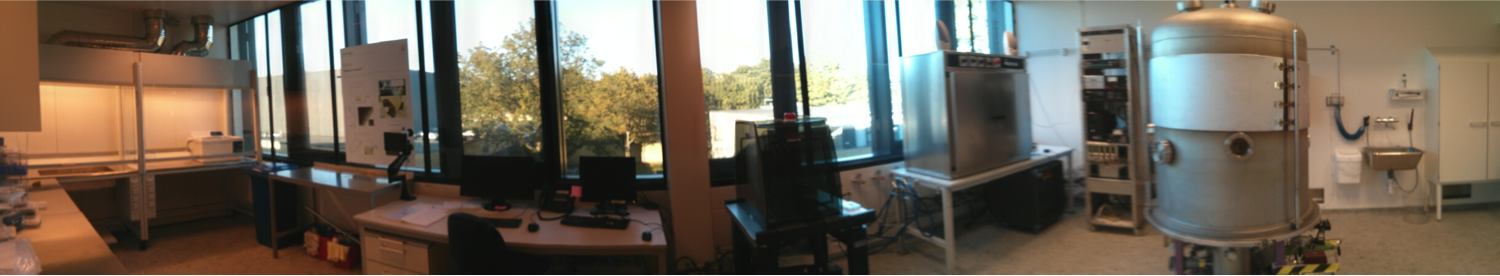
\includegraphics[width=\linewidth]{figures/chamber/multilab1.png}
  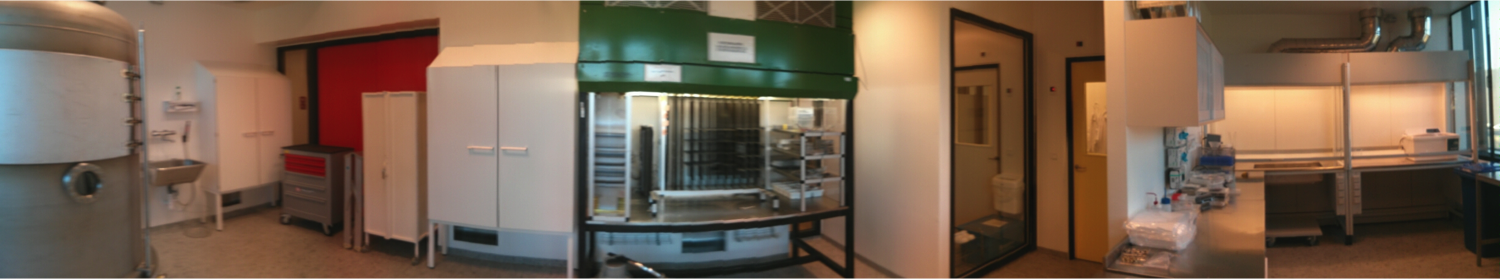
\includegraphics[width=\linewidth]{figures/chamber/multilab2.png}
  \caption{\footnotesize Panoramic view of the Multilab coating facility at DTU Space. Top right can be seen the bell-shaped coating chamber.}
  \label{fig:multilab}
\end{figure}

The vacuum chamber is the dominant piece of the laboratory and most of the computers, electronics and cooling in the lab is in some way connected to the chamber. Apart from the chamber, the lab consists of a downflow module, two fume hoods, a profilometer, a large clean room oven and various tables and cupboards (see figure \ref{fig:multilab}). Next to the lab is the Multilab Auxiliary Room, which houses the cooling heat exchangers and pumps, the rotary vane roughing pump, DC power supplies, and a large part of the extra storage needed for the lab. Additionally, there is a room in the basement that houses a ceramic oven that has a built in vacuum chamber, the room also serves to store hundreds of spare pieces of NuSTAR optic glass.

\section{Coating chamber}
The coating facility at DTU Space is arranged with vertical sputtering cathodes pointing outwards in a circular vacuum chamber, see figure \ref{fig:chamber}. Substrates are mounted on vertical mounting plates that are placed on a rotating ring in the sputtering chamber and the substrates pass in front of each cathode at a speed determined by the desired layer thickness.

\begin{figure}[htbp]
  \centering  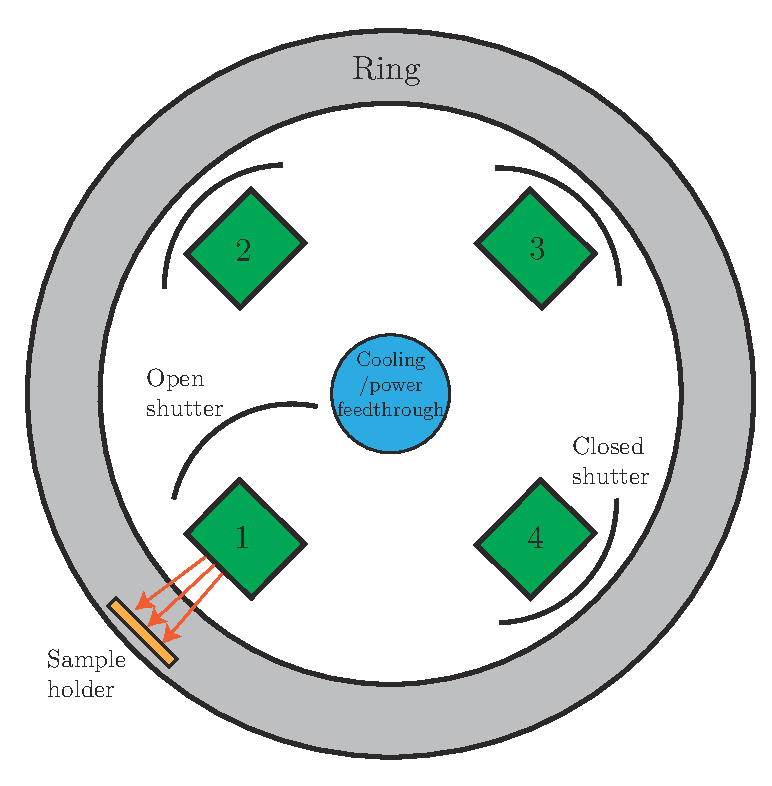
\includegraphics[width=0.5\linewidth]{figures/chamber/chamber.pdf}
  \caption{\footnotesize Diagram of the coating chamber at DTU Space, showing the principle of the rotating sample ring stage. Cathodes 1--4 (green) points outwards and can be covered with a shutter. Water cooling and power lines for the cathodes comes from the floor in the center of the chamber (blue) and connects to the top of each cathode with vacuum flex tubes. The sample (orange) is placed on a vertical plate that is mounted on the ring (grey). The ring rotates, so the samples move past the cathodes and gets coated with a film thickness related to the ring speed.}
  \label{fig:chamber}
\end{figure}

After chamber is closed, a roughing pump and a turbo molecular pumps evacuates the chamber to a pressure of $\leq2\cdot10^{-6}$ Torr before pure Ar gas is let into the chamber at a constant flow rate to ensure the fraction of other gases to be $<$0.1\%. The desired total pressure with Ar gas is $2.8\cdot10^{-3}$ Torr, which is as low as possible while maintaining plasma stability.

The chamber fits four cathodes at a time and the Multilab has six in total, so two can be serviced while the other four are in use. For most coatings, only two or three cathodes at a time are necessary for the same number of materials.

In the earlier software solution, all cathodes were switched on at the same time during deposition of a bilayer. That necessitated two cathodes running with the low-Z material while one cathode ran with the high-Z material in order to achieve the correct $\Gamma$ value and to have each cathode running in a possible power regime. A typical Pt/C  multilayer for NuSTAR required $\Gamma = 0.6$, which meant that 60\% of a material in a bilayer had to be carbon. Platinum and carbon has vastly different coating rates, so one cathode with Pt running at 150 W required two cathodes of C running at 900 W in order to achieve $\Gamma = 0.6$. With the new software only one cathode with each kind of material is necessary, but at the expense of a longer coating time.

\subsection{Magnetron cathodes}
The cathodes are the most important part of the chamber. They are 20 inches long and 1/2 inch wide planar magnetron cathodes made by Angstrom Sciences Inc. A diagram of the cathode can be seen in figure \ref{fig:cathodeintersection}. A copper (Cu) block acts as the cathode with a stainless steel shield around it, separated by teflon spacers. Inside the Cu block, three permanent magnets with alternating field directions supplies a magnetic field in front of the cathode. Water cooling and power lines are connected from the cathode through a flexible vacuum tube to water cooling and power supplies outside the chamber. The anode shield is grounded along with the rest of the chamber.

\begin{figure}[htbp]
  \centering  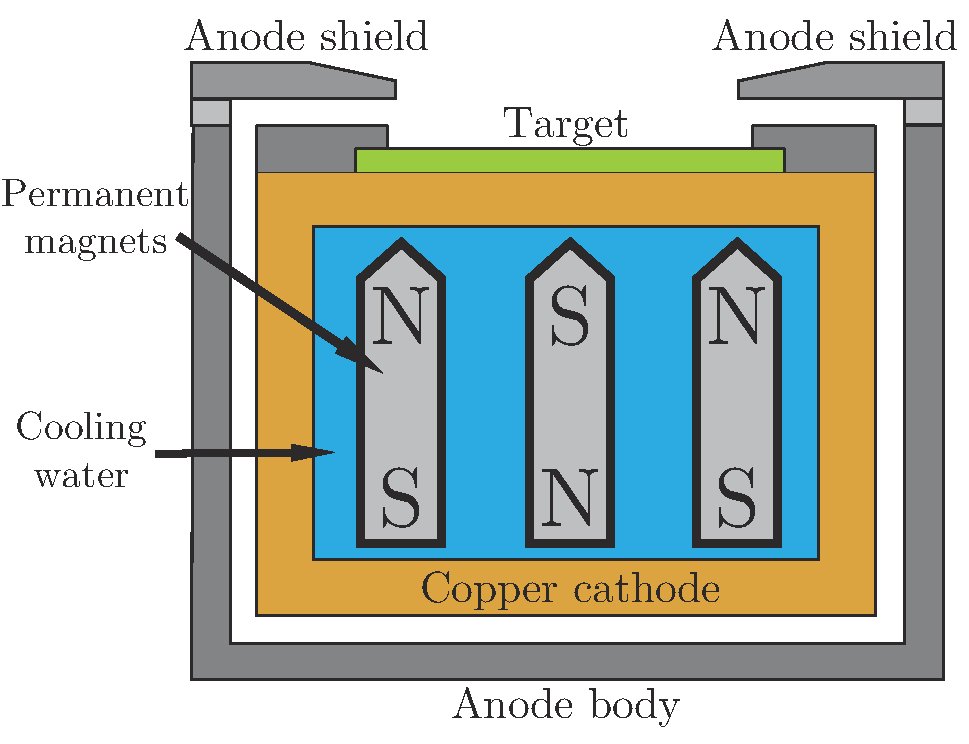
\includegraphics[width=0.5\linewidth]{figures/chamber/cathodeintersection.pdf}
  \caption{\footnotesize Cross-sectional diagram of a magnetron cathode used in the Multilab at DTU Space. }
  \label{fig:cathodeintersection}
\end{figure}

Materials for sputtering, called targets, are fastened to the Cu block using a stainless steel clamp. It is important for the target to have a uniform contact with the cathode, so the Cu block should be cleaned before fastening using cleanroom wipes and ethanol. For tougher blemishes, a micro-fine sanding sponge can be used to clean the surface followed by ethanol and cleanroom wipes.

Applying a voltage of -400 V to the cathode creates an electric field in front of the target. The Ar gas present in the chamber will be ionised in front of the cathode by the electric field, stripping an electron from the Ar atoms resulting in a plasma. The positive Ar$^+$ ions are accelerated towards the target, whereby the collision with the target create a sputtering of target atoms in a cone directed normal to the target surface, see figure \ref{fig:sputtering}. A substrate placed opposite the cathode will be coated with the sputtered atoms at a rate proportional to the electric current applied to the cathode.

\begin{figure}[htbp]
  \centering  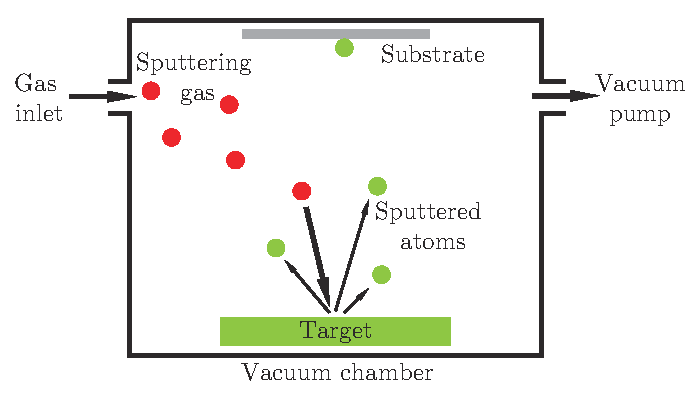
\includegraphics[width=0.6\linewidth]{figures/chamber/sputtering.pdf}
  \caption{\footnotesize Principle of sputtering. Sputter gas led into an evacuated chamber is forced to the surface of a target with a force that rips atoms from the material. The freed target atoms move away from the target and some hit a substrate opposite the target. }
  \label{fig:sputtering}
\end{figure}

Electrons stripped from Ar atoms are captured by the magnetic field lines from the permanent magnets in the Cu block. The electrons are moved back and forth across the target and occasionally hits neutral Ar atoms, which also become ionised and thereby sustain the plasma. The movement of electrons are from the center of the target to the outer edge, and as more Ar atoms are ionised in between those two points, the main erosion of the target during coating takes place in a so-called \emph{race track} around the target.
%
% !!!!!Something about the physics of sputtering!!!!!
%
% !!!!Thornton zone model?????!!!!!!

\section{Multilab control software}\label{sec:ml_software}
In the years before moving the DTU Space multilab to DTU campus, it became apparent that a completely new software solution was needed for the coating facility. The software controls all stepper motors (cathode shutters and sample ring), gas flow controllers,  cathode power supplies as well as pressure gauge communication.

The original software was made in Visual Basic 6, which Microsoft stopped supporting in 2008. Features that were not build into the software from the start was bolted on at a later stage, resulting in some files with thousands of lines of uncommented code. VB6 also has the drawback that it is single threaded, so only one command can be executed at a time which means that none of the instruments could be read for the log file if for instance the sample ring was moving. So checking whether there was a plasma dropout on a cathode was not possible while coating a layer, something that can take 30+ minutes.

Everything in the original software solution was controlled in a graphical user interface which made it easy to use, but would only allow for preprogrammed coating types to be made. When it came to make coating investigations for the Athena mission, the linearly graded coatings with top and bilayer required being in front of the computer during the process. For every layer, it was necessary to manually type in a new sample ring speed and start the movement. The coatings took on average 2-3 hours, so it became clear that a new solution was necessary.

\subsection{Considerations on the new software solution}
Considering the observations from above, a list of requirements for new software was made:

\begin{description}
  \item[Software should run on Linux] To remote control the coating facility in the old software solution, it was necessary to run a remote desktop to control the graphical user interface. The remote desktop requires a relatively large amount of internet bandwidth, something that is not always available. The new software should be controllable over a remote SSH connection using a Bash shell or similar.
  \item[Software should log continuously] Output from cathode power supplies, pressure gauges and flow meters should be read every 5 seconds during a coating. Between coatings, the pressure gauges should be read every 5 seconds and written to a web server. That allows for checking chamber status on a smart phone or computer connected to the internet.
  \item[A coating run should be described in a script] Instead of predefined coating types, the scripts make it possible to produce completely custom multilayer coatings.
  \item[Software should preferably be open source] Open source software is often well documented and flexible. An open source programming language with plenty of extra packages could be Python.
\end{description}

The first attempts at creating new software was directed at Python, since that is just about the most well-documented programming language on the internet, and also where I have the most experience.

It became clear after a while that the real problem was satisfying the second requirement in the list above. All instruments controlled by computer in the multilab are communicated with using serial connections, which will block a line until a command is received by an instrument and a response is returned. In some instruments the response time is up to a second and for the stepper motors, a response is not returned until movement is complete. That is the reason why the old software was unable to read any outputs during the movement of the sample ring.

Python is a single threaded scripting language, so all commands are executed sequentially. There are however software packages for Python that can spawn subprocesses from a queue and read the output of those into another queue. A specific package for multithreading serial communication is Twisted for Python, but after moderately successful attempts it was clear that the solution would be too difficult. The software should be flexible and making a multithreaded python solution with queue systems was both too much work and a bit like reinventing the wheel.

The choice in the end fell on SPEC, a software package for X-ray diffraction setups. SPEC is not open source, but requires a license. SPEC is widely used in synchrotron beamlines across the world, and also in the X-ray lab at DTU Space. It is an extremely flexible piece of software, specifically designed to talk to a wide range of instruments at X-ray beamlines. Many types of hardware can be controlled directly from SPEC without the need for drivers, since a direct hardware level communication protocol is build into the software. Commands are typed in on a command line, but can also written into text files (scripts) and the commands can then be executed sequentially by SPEC.

\subsection{Software architecture of new Multilab control program}
SPEC is, like Python, single threaded. There are however build-in procedures for communicating through the serial protocol and a range of other protocols. SPEC also has the ability to run as a server so commands can be issued to the software using sockets on the system level. By running three separate instances of SPEC at the same time, it became possible to constantly communicate with instruments, write to a logfile, and control the chamber from a main program. The software is set up like the following:

\begin{description}
  \item[SPEC (main program)] The main program, where user-level commands can be typed in. Coating macros are executed from this program. The program has direct control with stepper motors using text-based serial communication\footnote{To use SPEC most efficiently, a direct hardware-level communication should be initiated between SPEC and motor controller. However, the motor controller would have to be supported on the hardware-level by SPEC, which is not the case for the current hardware in the Multilab. If a new motor controller is procured, it should be on the list of hardware supported by SPEC. (\emph{http://www.certif.com/hdwdevices.php?family=motor})}.
  \item[ControlServer] The control program. It has direct access to cathode power supplies, gas flow controllers and pressure gauges. SPEC and LogClient will get status and control the instruments through ControlServer by socket commands.
  \item[LogClient] The logging program. It gets data from the ControlServer every five seconds and writes the data to a file. If a coating is starting, it will make a new folder in the \verb'~/logs' directory named by time and date. In that directory it will make a log file (\verb'logfile.txt') for the coating and also a log of the commands typed in by a coating macro (\verb'coatinglog.txt').
\end{description}

These three programs run continuously side-by-side, and will make sure that there are no interruptions in the logging during a coating run. Each command to control any part of the instruments are described in the \verb'site.mac' macro files of each program and auxiliary macro files for e.g. power supplies and pressure gauges. All commands are divided into system-level and user-level commands. System-level commands are called like this:

\begin{verbcode}
  SPEC> output = getpoweroutput(#)
\end{verbcode}

This command will get the output of cathode \verb'#' and put the result in the variable \verb'output'. The system-level commands \emph{can} be used by the user, but \emph{should not}. Instead they are used inside user-level command macros, so a user-level command looks like this:

\begin{verbcode}
  SPEC> getpoweroutput 1
  Current power output of cathode 1: 450 W
\end{verbcode}

This makes it easier to type commands into SPEC, as commands can be autocompleted by using the tabulator key. If a command needs one or several parameters following it and not enough/too many are given, it will respond with an error and a description of the parameters needed.

Log files produced continuously by the LogClient program are fetched by a web server at DTU Space that will make a plot of pressure and cathode power output every 30 seconds. A plot from Sept. 14th 2014 can be seen in figure \ref{fig:chamber_pressure}. The logfile holds up to 50,000 lines of data, which corresponds to $\sim$3 days of data collected every five seconds. In the plot can be seen both the curve corresponding to the cold cathode pressure gauge (red line) and the baratron pressure gauge (green line). The cold cathode works well at both low and high pressure, but some of the functional parts can be coated over during a coating, so a valve closes off to that gauge during coating. The baratron only works between $10^{-1}$ Torr and $2\cdot10^{-4}$ Torr, but is more precise and also works during a coating.

\begin{figure}[htbp]
  \centering
    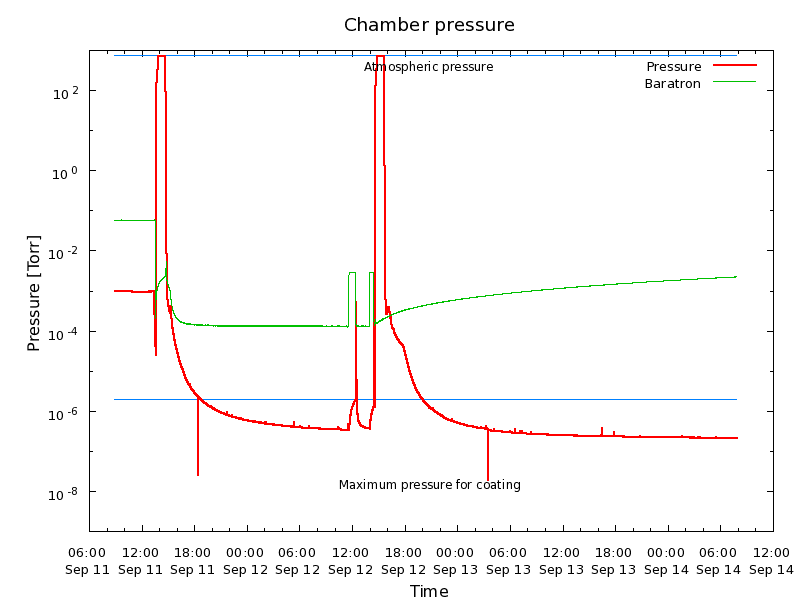
\includegraphics[width=0.8\linewidth]{figures/chamber/pressure.png}
  \caption{\footnotesize Plot representing the output from the continuous logging of chamber pressure. Red line is the pressure measured by a combined cold-cathode/penning gauge, that works well under both atmospheric pressure and low pressure. It will not function well during a coating. Green line is the MKS Baratron pressure gauge, that is precise in the $2\cdot10^{-4}$ -- $5\cdot10^{-2}$ Torr range.}
  \label{fig:chamber_pressure}
\end{figure}

The web server that continuously fetches the log file from the coating computer also gets information from the X-ray measurement computer in the basement. Information about measurement status and progress is posted to the same web site. This makes it possible to get the status about all the labs by a quick glance to the web site. The script running on the web server also has the option to send out a mail to pre-defined recipients if the pressure in the chamber is low enough to start a coating. This proved handy during the NuSTAR coatings, where coatings had to be started in the middle of the night. The web site and script running on the web server were produced during the NuSTAR coating campaign to make the production process easier.

The cathode shutters and ring are all controlled by the same motor controller, and is communicated to over the same serial cable. That is however opaque to the user. In order to open or close a specific shutter, the command \verb'osh #' or \verb'csh #' should be given for opening and closing shutter \verb'#', respectively. Alternatively, all shutters can be opened or closed using \verb'openallshutters' and \verb'closeallshutters'. The ring can be controlled using the commands \verb'mra speed angle' or \verb'mr speed steps', the first of which moves the ring at the speed given in steps/sec. at an angle given in degrees. The second does the same thing, except for changing the angle for steps. The motor controller has 668,000 steps in a complete rotation of the ring in the chamber and the speed of the ring should be between 0 and 15,000 steps/sec, otherwise the movement precision decreases. In a coating macro, the command \verb'mra speed angle' is used extensively as the main method to move the samples past the cathodes.% In chapter \ref{chap:multilab_details}, an extensive list of commands made for the control software can be found.

\subsubsection{Interfacing with cathode power supplies}
The power supplies used to run the cathodes in the multilab consist of two Advanced Energy Pinnacle 5/5 DC power supplies and one Advanced Energy Pinnacle Plus+ 5/5 pulsed-DC power supply. Each power supply has two channels, so can run two cathodes at same time. In order to communicate with power supplies, a special protocol running over serial has to be used. All other instruments in the multilab are communicated with by ControlServer and SPEC using basic text commands send over a serial connection.

The protocol is made for connecting all power supplies to the same serial connection, but in the multilab they are connected separately. The protocol requires each command to be packaged in a binary packet that includes power supply hardware address, length of packet, command, data and finally an XOR of the entire packet so the receiver can verify that the whole packet is there. The design of the packet can be seen in figure \ref{fig:ae_packet}. In the header, which is 8 bits long, the first 5 are the address of the power supply (set with a DIP switch on the back) and the remaining 3 bits describe the length of the packet. If the length in the header is set to 7 (111 in binary), the 'optional' byte is used to describe the actual length of the packet. The 'command' byte is a number between 0 and 255 (0 and FFh) in hexadecimal numbers. The 'checksum' byte is an XOR of the entire packet up until the 'chekcksum' byte. When the receiver gets a packet, it will do an XOR of the entire packet including the 'checksum' byte and if the result is 0, the packet is approved and processed.

\begin{figure}[!h]
  \center
  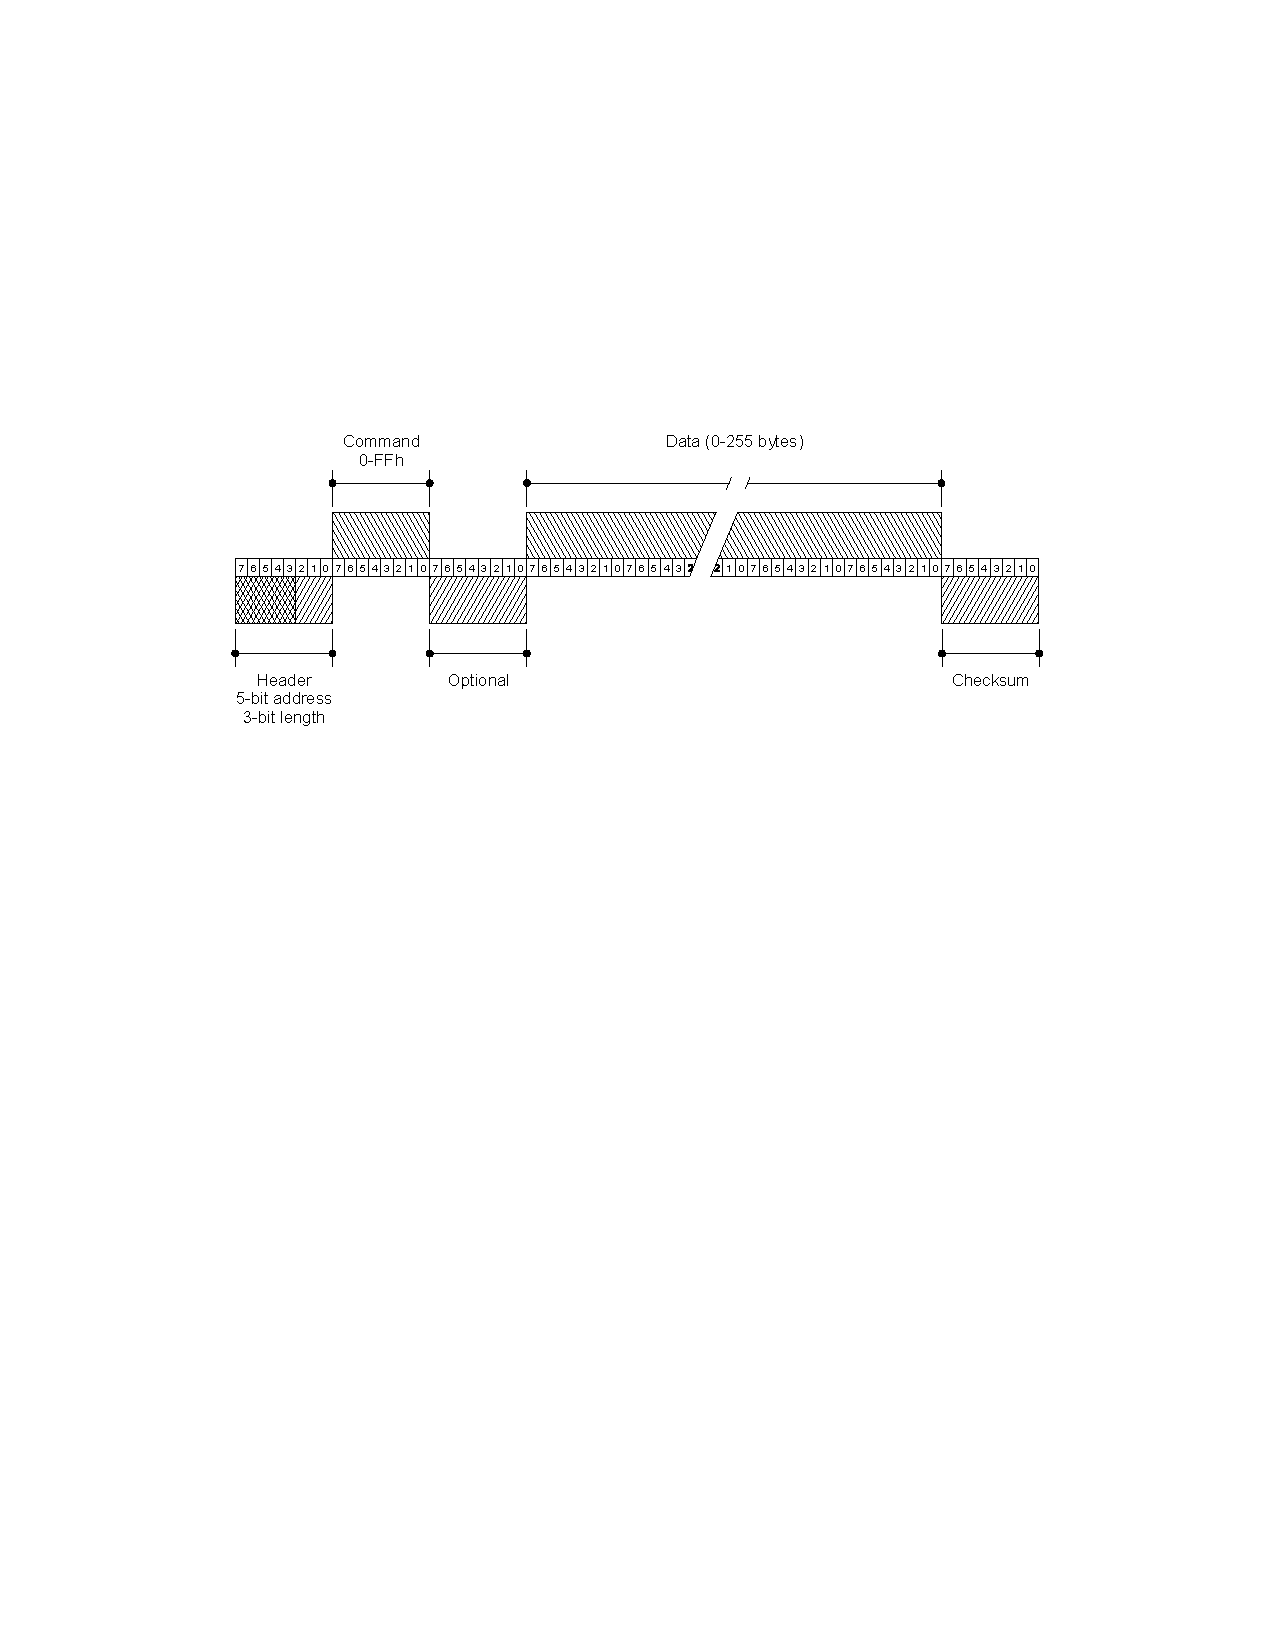
\includegraphics[width=0.9\linewidth]{figures/chamber/ae_packet.pdf}
\caption{\footnotesize Schematic of the principle of transmission data packets in the Advanced Energy communication protocol. Each number on the white line corresponds to one bit in the data packet, eight bits equals one byte. From \cite{Anonymous:zazNQqcS}}\label{fig:ae_packet}
\end{figure}

This packet architecture is used to communicate back and forth between the ControlServer program and the power supplies. If a packet is approved, an ACK is send back in the form of the hex code 06h. The commands for the power supplies can either be to retrieve current status of some parameter, to set a parameter on the power supply, or to execute a command on the power supply. The entire communication protocol is transparent to the user and all user-level control of the power supplies can be achieved by user-level commands only.

\subsubsection{Coating macro}
To produce a coating in the multilab chamber, a coating macro can be typed up and started in the main SPEC program as soon as the pressure is low enough ($\leq2\cdot10^{-6}$ Torr). An example of a simple coating macro, \verb'coat_singlelayer', can be seen here:

\begin{verbcode}
  def coat_singlelayer '
        if ($# != 1) {
                eprint "Start coating of singlelayer.\n"
                eprint "Usage: coat_singlelayer v(cath3)"
                exit
        }
        coating_start_log
        closevalve
        setflow 1 88
        openflow 1
        openmainflow
        print("Waiting for Ar flow to settle.\n")
        print("(60 seconds).\n")
        sleep(60)
        setpower 3 450
        print("Starting coating.\n")
        mra 90 10000
        sleep(2)
        pson 3
        sleep(5)
        osh 1
        print("Coating material 1, all plates.\n")
        mra -360 $1
        sleep(2)
        csh 1
        sleep(1)
        psoff 3
        mra -90 10000
        sleep(2)
        print("Coating over. Closing flow valve.\n")
        closemainflow
        closeflow 1
        openvalve
        coating_stop_log
\end{verbcode}

Each step in the macro is described here:

\begin{description}
  \item[Error check] The macro starts out with an \verb|if| statement to make sure that there is one parameter after the user has called the macro.
  \item[coating\_start\_log] Sets the variable \verb|coating_starting=1| in the LogClient program and lets it know that it is time to start a log for a new coating.
  \item[closevalve] Closes valve to the cold cathode pressure gauge.
  \item[setflow 1 88] Sets flow output on flow controller 1 to 88 SCCM.
  \item[openflow 1] Opens flow controller 1.
  \item[openmainflow] Opens flow controllers to chamber.
  \item[Text output to user] Feedback should be given to user throughout the coating.
  \item[sleep(60)] Macro will wait for 60 seconds to let the pressure settle at $\sim$2.8 mTorr.
  \item[setpower 3 450] Power output is set to 450 W on power supply output 3, the first output on the second power supply.
  \item[mra 90 10000] Ring is moved 90\degr\ at a speed of 10,000 steps/sec. so the first sample is right before cathode 1.
  \item[pson 3] Power supply 3 is turned on.
  \item[osh 1] Shutter 1 to cathode 1 is opened.
  \item[mra -360 \$1] Ring is moved 360\degr\ at the speed given by the parameter which is set by the user when calling the macro.
  \item[csh 1] Shutter 1 is closed after ring is done moving.
  \item[psoff 3] Power supply 3 is turned off.
  \item[mra -90 10000] Ring is moved back to start position.
  \item[closemainflow] Main flow to flow controllers is turned off.
  \item[closeflow 1] Flow controller 1 flow is turned off.
  \item[openvalve] Valve to cold cathode pressure gauge is opened.
  \item[coating\_stop\_log] Sets the parameter \verb|coating_starting=0| in the LogClient program, which stops logging for that coating.
\end{description}

The macro will coat all samples in the ring with one layer of the material on cathode 1 at the speed given by the parameter after the macro call. Macros in SPEC are given in a C-type language and many types of loops and statements are implemented. The comprehensive manual for SPEC gives a good overview.

If the user wants to make more complicated multilayers, adjusting the macro example above into a graded-d type coating can of course seem daunting. For that reason, subfunctions are implemented that will coat e.g. 90\degr\ of the ring with cathode 3. The principle of the subfunction is as follows:

\begin{enumerate}
  \item From the start position of the ring where sample 1 is placed, the ring will move sample 1 between cathode 2 and 3.
  \item Turn on cathode 3 and open shutter.
  \item Move ring 90\degr\ given by input parameter.
  \item Close shutter 3 and turn off cathode.
  \item Move ring back to start position.
\end{enumerate}

The sample can then be coated by another cathode afterwards. If a larger batch requires coating at the same time, there are similar subfunctions for moving 180\degr\ and 360\degr.

The software also makes it possible to coat four different samples with four different coatings in the same coating run. By placing the samples at four different corners of the ring, each sample can have a coating applied separately. Flexible macros for that purpose are not yet implemented, but a template that can be changed into a specific purpose is the macro
\begin{verbcode}
  SPEC> coat_n_bilayers_4plates
\end{verbcode}
along with subfunction e.g.
\begin{verbcode}
  SPEC> abilayer_4_plates_c2c4($2,$3,$4,$5,$6,$7,$8,$9)
\end{verbcode}
that will coat four different constant-d coatings using cathode 2 and 4. It is possible to change any parameter for the power supplies or flow meters between each sample, so testing out a parameter space becomes significantly faster with this system.

For linearly graded-d coatings, an example is given below that shows the flexibility of the SPEC macro language.

\begin{verbcode}
  for (j=0;j<nlayers;j++){
    printf("\nStarting layer %g.\n",j+1)
    dlayer = dmin+(j)*(dmax-dmin)/(nlayers-1)
    dlayer1 = dlayer*gamma
    dlayer2 = dlayer*(1-gamma)
    speed1 = int(1/((dlayer1-sicorr)/sifact))
    speed2 = int(1/((dlayer2-wcorr)/wfact))
    coat_cath2_180 speed2
    coat_cath4_180 speed1
    }
\end{verbcode}

By defining \verb|nlayers| as the number of layers, \verb|dmin|, \verb|dmax| and \verb|gamma| of the coating along with calibration factors, the macro will for every layer calculate the speed for both materials and coat the correct thickness. Calibration factors are calculated as seen in section \ref{sec:coating_calib} where $a$ for W is \verb|wfact| and $b$ is \verb|wcorr|. The same principle can be used in other types of graded-d coatings, e.g. power-law gradings with $a$, $b$ and $c$ defined in $d_i = a/(b+i)^c$, where $d_i$ is the d-spacing of the i'th layer.

\section{X-ray lab source at DTU Space}
Measurements at DTU Space were done with a reflectivity setup consisting of a rotating Cu-anode providing X-ray photons for two beams. One beam is used for reflectivity measurements and the other can be set up for measuring curvature in glass substrates.

After the source, along the z-axis, is placed two slits, a monochromator, an attenuator, on more slit, the sample holder and finally the detector, see figure \ref{fig:xraysetup}. The first two slits ensures that only a narrow beam hits the monochromator, which then reflects only photons around the Cu K$_{\alpha_1}$ emission line (8.047 keV) by reflecting the beam on two Ge crystals at an angle where Bragg reflection only allow photons of that energy. The beam continues through the next two slits, thereby minimizing divergence and also filters out a large part of unwanted reflections from the monochromator to ensure a narrow bandwidth. The attenuator ensures that the beam intensity is not too large, thereby saturating the detector.

\begin{figure}[!h]
  \center
  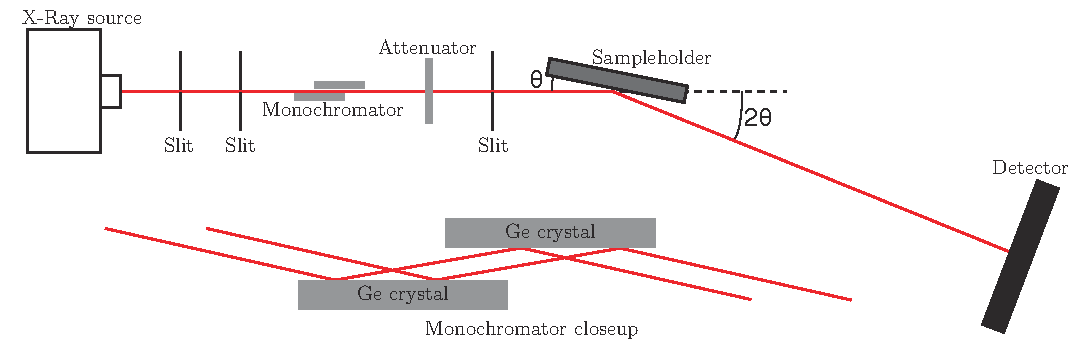
\includegraphics[width=0.8\linewidth]{figures/chamber/xraysetup.pdf}
\caption{\footnotesize Diagram of the X-ray setup at DTU Space. X-ray photons from the source goes through two slits, a monochromator, an attenuator and one more slit before hitting the sample. The reflected photons from the sample travel to the detector which is rotated at a $2\theta$ angle. Below: The monochromator that consists of two Ge crystal that reflect only a given wavelength on the (111) surface using the Bragg principle.}\label{fig:xraysetup}
\end{figure}

The sample holder consists of a slab of flat perforated ceramic material, a vacuum chuck, mounted vertically. It is connected to a pump, which allows flat substrates, like pieces of Si-wafer, to stick very firmly to the stone slab. This method of sample mounting makes it possible to change samples very fast and easy between measurements. The sample holder is centered and mounted on a rotating stage, $\theta$, and can also move in and out of the beam along the x-axis.\\
After the sample holder, 995 mm further along the z-axis is a 10 cm wide 2D methane-gas detector mounted on a rotating stage, $2\theta$. It is centered on the same axis as $\theta$, allowing the detector to move 90\degr around the sample while maintaining a focus on the same spot. The detector has 2000 channels along the x-axis of the beam; 100 channels are used during a measurement, giving a horizontal detector aperture of 2 cm.

\section{Coating calibration}\label{sec:coating_calib}
To deposit a coating with the correct film layer thicknesses on a substrate, a calibration of the material combination is required. Four samples of 10 bilayer films are coated using the two materials. Each sample is placed on a separate mounting plate and each coated with a different thickness of both light and heavy materials. The samples are then measured using XRR and compared to an IMD\cite{Windt:1998tb} model fit to get bilayer thickness (d-spacing) and light/heavy material fraction ($\Gamma$) as seen in figure \ref{fig:irb4c-fit}.

\begin{figure}[!h]
  \center
  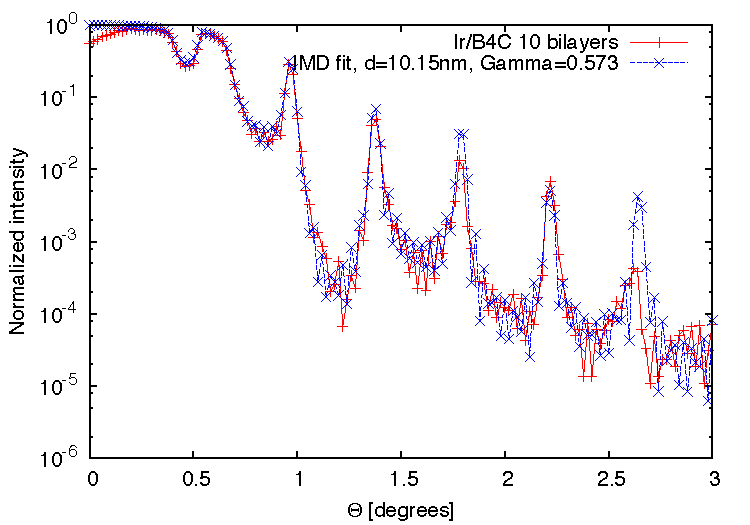
\includegraphics[height=7cm]{figures/chamber/si5811-fit.pdf}
\caption{\footnotesize XRR measurement of a 10 bilayer Ir/B$_4$C coating to calibrate for SPO coating. The measurement is fitted with an IMD model to determine d-spacing $\Gamma$.}\label{fig:irb4c-fit}
\end{figure}

The result for each sample is used to get the specific thickness of a material when coating with a given speed. Each result from the IMD model fitting is put into a table like the following:

%\begin{table}[!h]
\begin{center}
\begin{tabular}{c|c|c|c|c}
Sample & speed (Ir) & speed (B$_4$C) & d-Ir [nm] & d-B$_4$C [nm] \\
\hline
si5809 & 2623 & 473 & 2.42 & 2.54 \\
si5810 & 1445 & 338 & 3.21 & 3.88 \\
si5811 & 1011 & 236 & 4.33 & 5.81 \\
si5812 &  674 & 158 & 6.40 & 8.85 \\
si5813 & 281 & 225 & 14.55 & 7.49
\end{tabular}
\end{center}
%\caption{\footnotesize Calibration samples coated with 10 bilayer Ir/B$_4$C multilayers of different thickness. Each sample is measured using XRR and fitted to an IMD model. \label{tab:AFMsamples}}
%\end{table}

The d-spacings for a given material are plotted as a function of the inverse speed of the sample ring (v$^{-1}$) and fitted with a linear regression as seen in figure \ref{fig:calib-fit}. The $a$ and $b$ values of the linear regression are used directly to determine the speed of the sample ring, $v_{\mathrm{B}_4\mathrm{C}}$, to coat e.g. B$_4$C with a thickness of $d_{\mathrm{B}_4\mathrm{C}}$ like so:

\begin{eqnarray}
	v_{\mathrm{B}_4\mathrm{C}} = \frac{a}{d_{\mathrm{B}_4\mathrm{C}}-b}.
\end{eqnarray}

\begin{figure}[!h]
	\center
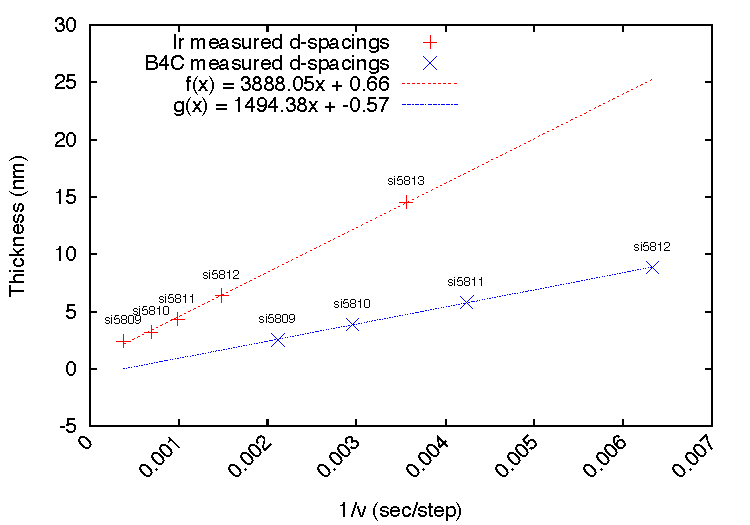
\includegraphics[width=0.8\linewidth]{figures/chamber/calibration_plot-ir-b4c.pdf}
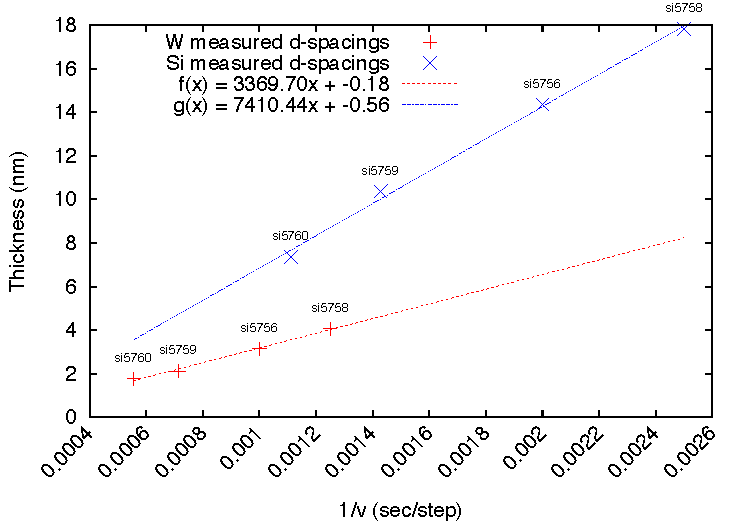
\includegraphics[width=0.8\linewidth]{figures/chamber/calibration_plot-w-si.pdf}
\caption{\footnotesize Linear regression fits of calibration samples for Ir/B$_4$C (top) W/Si (bottom). Each datapoint is the XRR measured thickness of one material layer in a sample.}\label{fig:calib-fit}
\end{figure}

%!TEX root = /Users/andcj/Dropbox/Documents/PhD/Thesis/phdthesis.tex
\chapter{Coatings for Athena}\label{chap:Athena_coatings}
In this chapter are described developments and investigations in the coating technology required for the European Athena mission. The work started in spring 2011, now involves five employees and students at DTU Space, and is still ongoing.

The first part of the chapter describes the Athena telescope and optics technology. Afterwards is a description of the X-ray reflective coating investigation carried out at DTU Space, starting with the baseline coating and stress investigation in \cite{Jakobsen:2011vd}. Proceeding that is the work based on different optimization techniques multilayer coatings, namely reactive sputter deposition and pulsed-DC sputtering. The coating lab acquired a pulsed-DC power supply specifically for the Athena coating investigations, but no improvements were found. Additionally, a number of problems showed up with the new power supply and the causes were not clear. Reactive sputtering investigations revealed major problems with some material combinations that included B$_4$C, which became apparent after long term storage investigations. In the end, the baseline material combination that was initially proposed for Athena was found to be the best-performing and most stable solution.

The last part of this chapter (section \ref{sec:Athena_upscaled}) is based on a report written to ESA on the coating production facility requirements for the original Athena mission proposed in 2012. A significant effort will have to be put into mass production for the Athena optic to be realised. The section points out the cost and timetable of such an effort.

\section{The European Athena mission}
Design and development of the Athena mission was started already in the 90's as first a European mission (XEUS) with the intent to make a high resolution X-ray telescope with a large effective area. In 2008 it merged into IXO (International X-ray Observatory), a European/American/Japanese collaboration. In 2012 after some years of global financial crisis, the collaboration fell apart as a result of down-scoping of space-related projects.

The European Space Agency (ESA) continued development of a smaller mission using technology that had already been in development for IXO for almost a decade. The mission was Athena (Advanced Telescope for High-ENergy Astrophysics)\cite{Barcons:2012va}, but was not selected as the 2022 large (L1) mission by ESA. Development continued under the Athena+ name, and the project was eventually selected for the L2 mission to be launched in 2028. To avoid confusion, Athena+ was after selection renamed to Athena.

\begin{figure}[!h]
  \center
  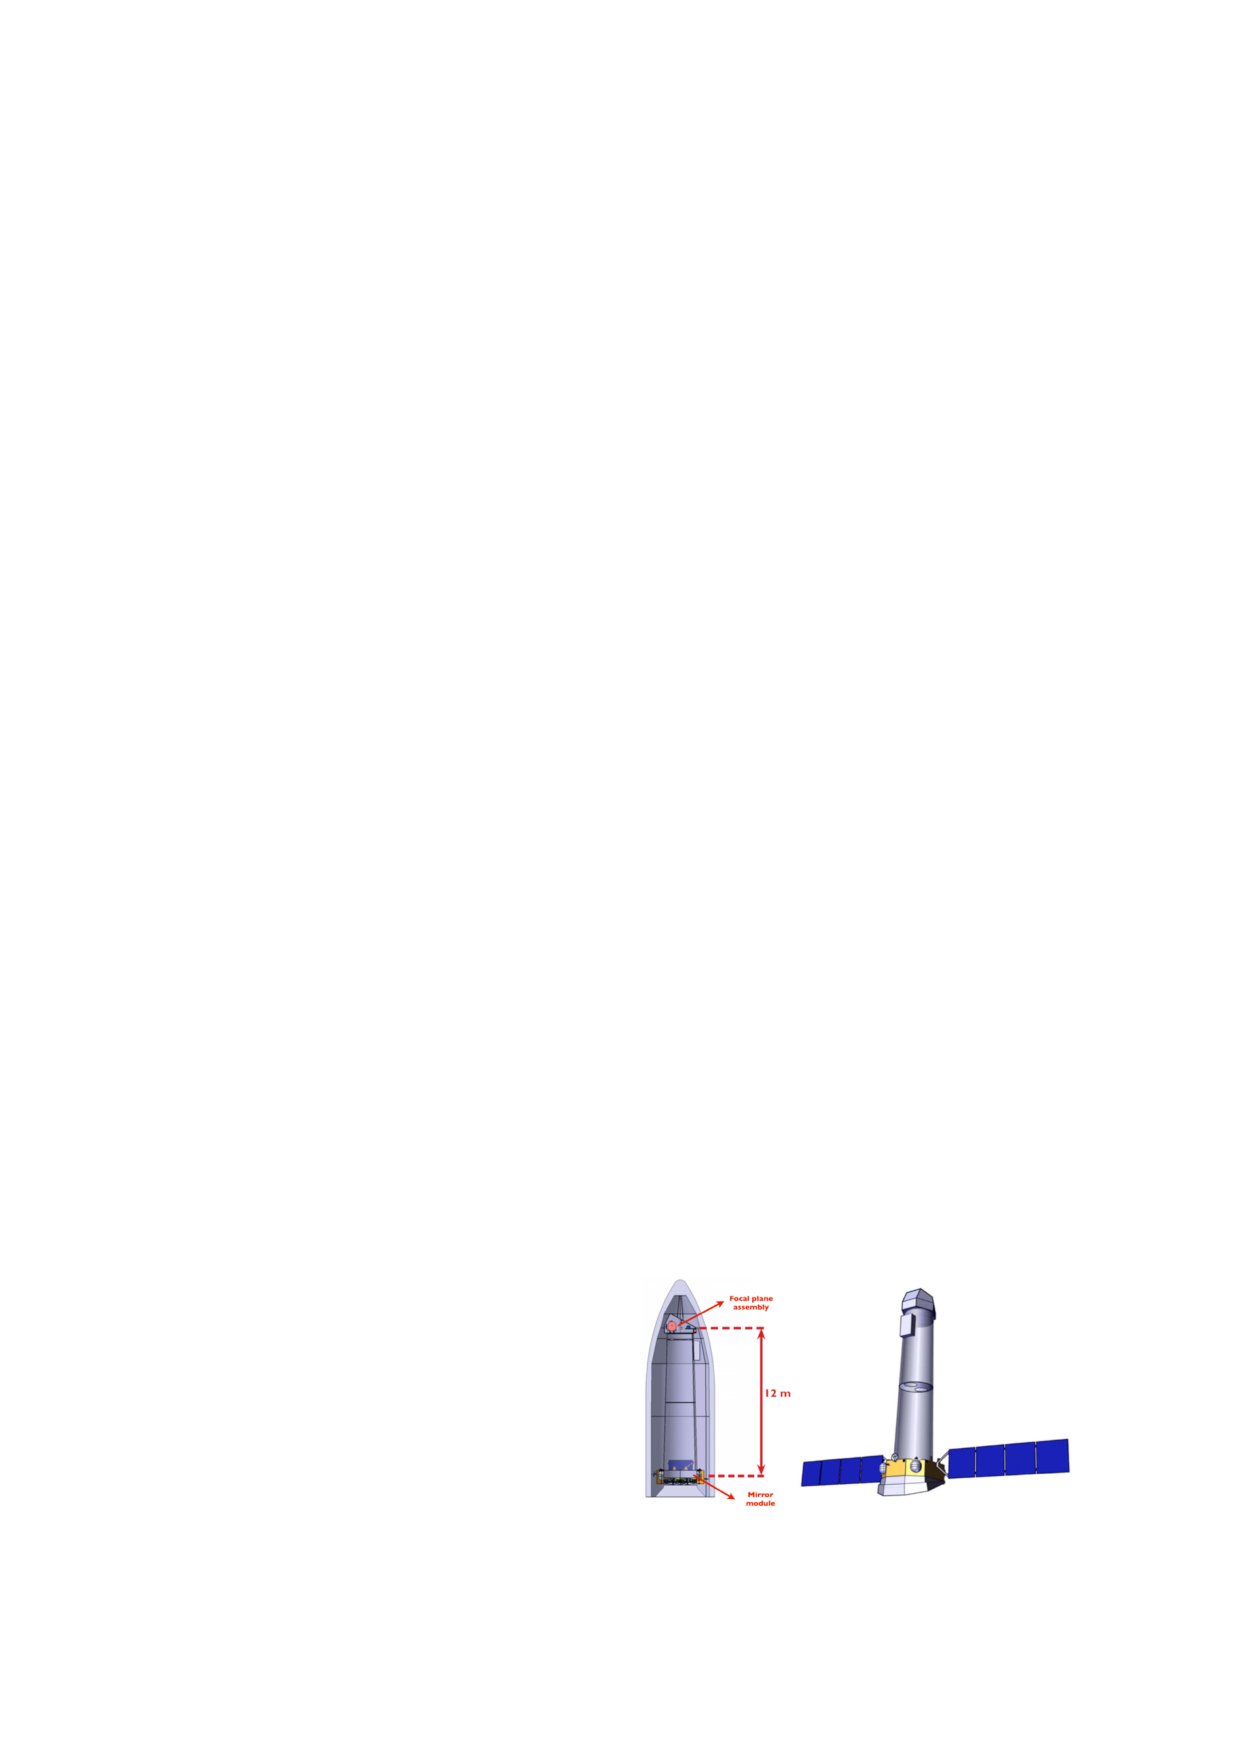
\includegraphics[height=8cm]{figures/athena/athena_telescope.pdf}
\caption{\footnotesize Illustrations of the Athena X-ray telescope. \textbf{Left:} Inside Ariane V fairing. \textbf{Right:} In space with extended solar panels. The optic is in the bottom end. (from \url{www.the-Athena-x-ray-observatory.eu}).}\label{fig:Athena_telescope}
\end{figure}

The theme of the 2028 L2 mission is \emph{The Hot and Energetic Universe}, which aims to answer the questions:

\begin{enumerate}
  \item How does ordinary matter assemble into the large scale structures that we see today?
  \item How do black holes grow and shape the Universe?
\end{enumerate}

The first question might be answered by looking at galaxy clusters from their formation at $z\sim$ 2--3 until present day. As the structures grow over time due to accretion of hot gas they eventually become the largest bound structures in the universe. To understand the growth, it is necessary to get information about velocity, thermodynamics and chemical composition of the gas. The high temperature of the gas results in considerable amounts of X-ray emission and the goal is to measure the spectroscopic output of galaxy cluster from $z=$1 and beyond. In order to study the morphology of such clusters and in order to get spectroscopic information, a telescope with a large collecting area and good spatial resolution is required.

The second question could be answered by looking at the supermassive black holes at the centers of galaxies. By looking at the epoch where the first galaxies were forming at $z=$ 6--10, the growth of the black holes can be tracked. However, that will require survey capabilities $\sim$100 times better than available with current X-ray telescopes. It will require a wide field of view as well as high sensitivity, which depends on large throughput and good spatial resolution.

In conclusion, the mission calls for high energy and spatial resolution spectroscopic observations and deep wide-field X-ray imaging. The performance in these areas should greatly exceed instruments currently in use such as Chandra and XMM-Newton as well as future missions such as Astro-H and eRosita. The improvements are to be realised with an effective area of 2 m$^2$ at 1 keV, 5'' angular resolution and 40'x40' wide field-of-view\cite{Willingale:2013vo}.

\subsection{The Athena reflective coating baseline}
The baseline coating for Athena is an Ir/B$_4$C single bilayer. The Ir will reflect higher energy X-rays in the 0.1--10 keV energy range, and the B$_4$C top layer will reflect lower energies. The B$_4$C material is able to withstand the C-C bond-breaking chemical solutions applied in the last step of the lithographic process (described in section \ref{sec:litho_process}), while at the same time being a very light material. The low electron density gives B$_4$C a very good reflectivity at energies 0.1--$\sim$3 keV. In investigations done by Lumb et al are results of measurements on an Ir/C single bilayer, where the C overlayer results in a doubling of effective area of the former XEUS telescope at 2--4 keV\cite{Lumb:2007vt}. This effect is due to the lower photoelectric absorption in low density materials such as boron and carbon in total reflection mode\cite{pareschi:2004dd}.

The Ir/B$_4$C combination does however have some drawbacks, especially high compressive film stress. Additionally, the Ir/B$_4$C material combination is not described in the literature, so the interplay between the two materials in both the short and long term is relatively unknown. In appendix \ref{pap:PREL_Athena} can be found a paper from 2011 that investigates the baseline Athena coating along with solutions to handle the film stress. In section \ref{sec:Athena_cr_impro} is a continuation of the investigation into stress improvements.

\subsection{Coating optimisations for Athena}
To improve on the Athena baseline coating, a range of alternative material combinations were investigated using computer optimisation with Markov chain Monte Carlo methods by Desiree D. M. Ferreira at DTU Space. A number of optimised coating recipes were produced for each material combination and the actual coatings were subsequently produced on SPO substrates in the coating lab at DTU Space. In appendix \ref{pap:Athena_2012} (see also \cite{ferreira2012Athena}) can be found a paper from 2012 on some of the optimizations and investigations done on coatings applied to SPO substrates.

The material combinations investigated in this thesis are:

\begin{description}
  \item[Ir/B$_4$C single bilayer (baseline)] The baseline material combination that yields the effective area of 2 m$^2$ at 1 keV for Athena.
  \item[Ir/B$4$C multilayer] An improvement on the baseline using the same material combination. A stack of bilayers is designed to improve the reflectivity around 6 keV while still retaining the baseline effective area.
  \item[W/B$_4$C multilayer] A combination with lower stress and cheaper materials than the Ir/B$_4$C multilayer.
  \item[Pt/B$_4$C single bilayer] A backup of the baseline material combination if the stress proved to be too high for the SPO substrates.
\end{description}

\subsection{Athena optics technology}\label{sec:Athena_opt_tech}
ESA has for the past decade been working on a radically new optics technology for future X-ray missions, the Silicon Pore Optics (SPO)\cite{Barcons:2012va,Collon:2010bp,Collon:2006ky,Collon:2010bp,Collon:2006ky,Beijersbergen:2004cc}. By using silicon wafers, cut into rectangular shapes (diced) and with grooves cut into the underside, a high collecting area can be achieved with very low mass and at the same time achieve angular resolution better than NuSTAR-like glass.

\begin{figure}[!h]
  \center
  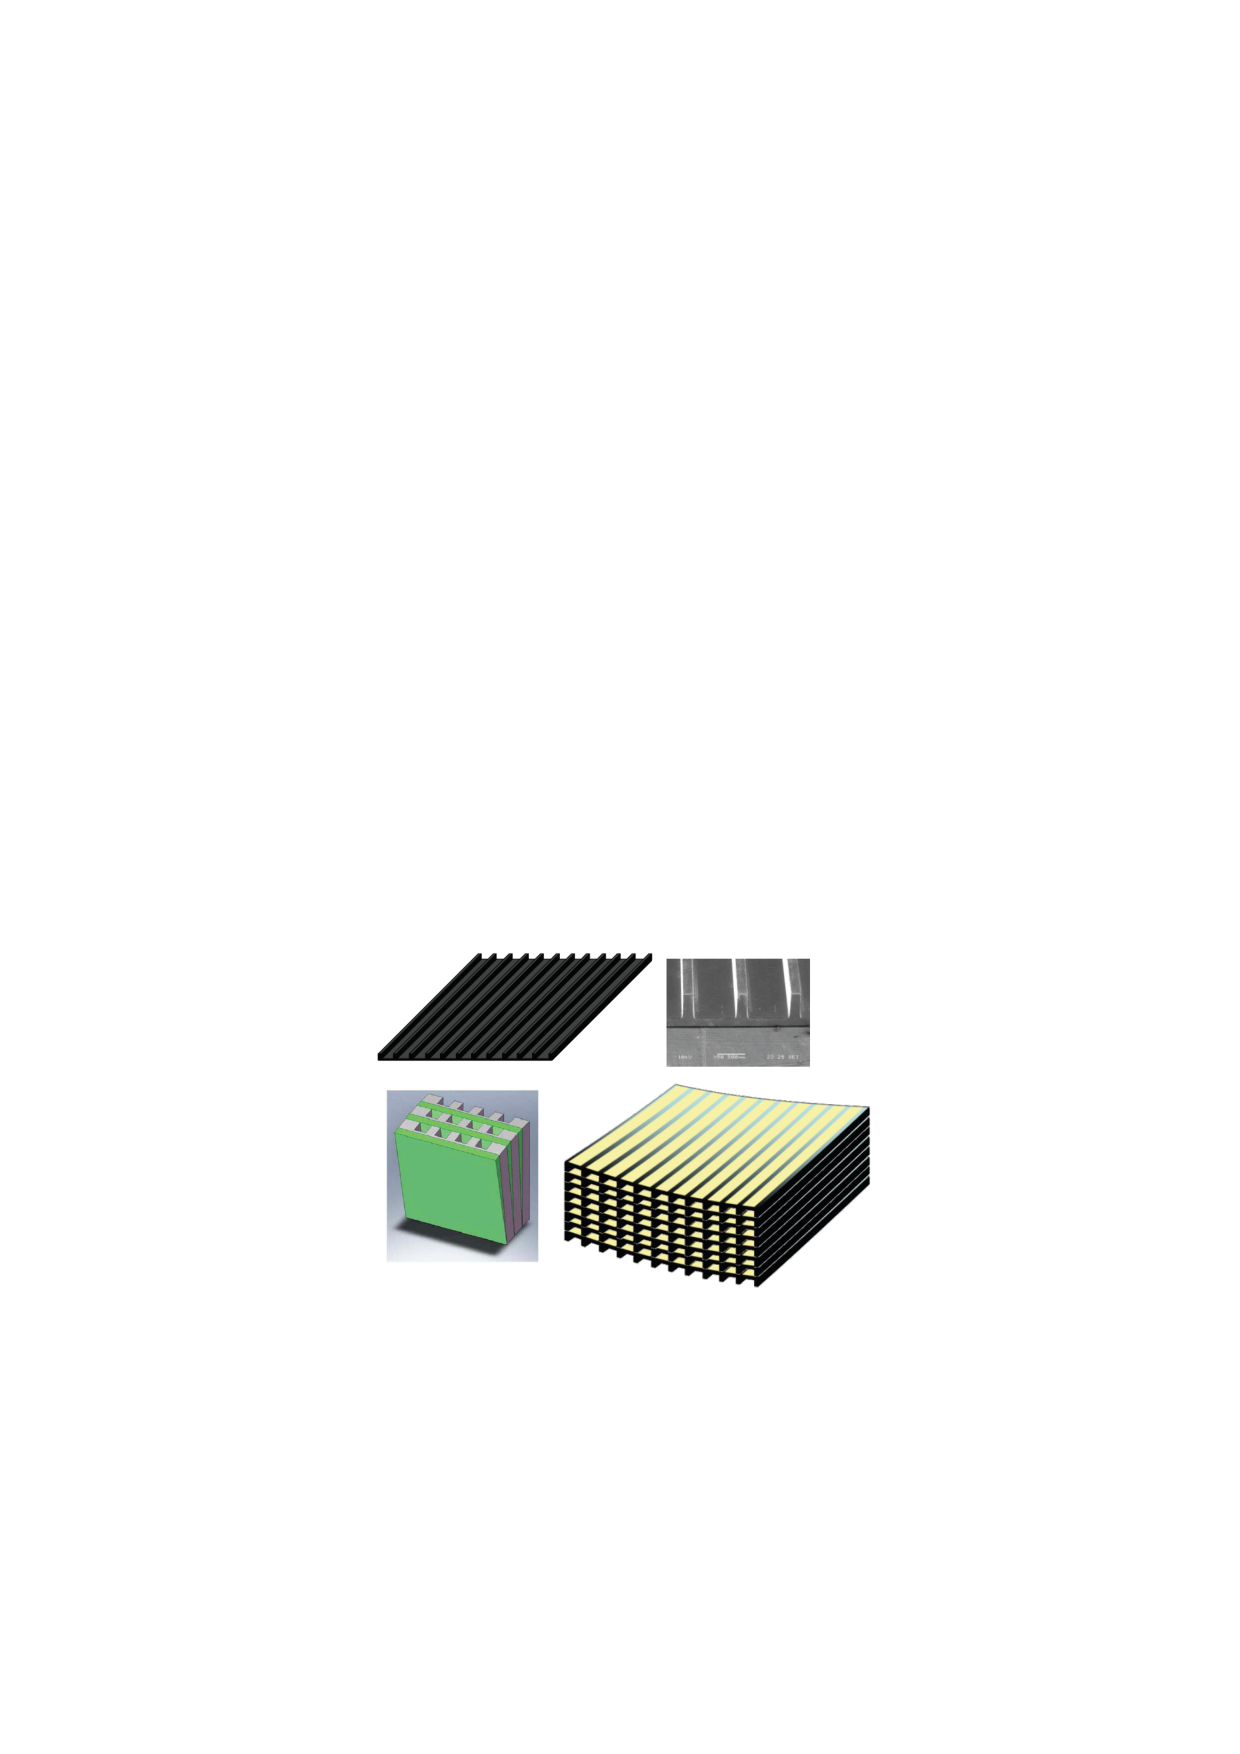
\includegraphics[height=8cm]{figures/athena/spo_principle1.pdf}
\caption{\footnotesize Principles of the Silicon Pore Optic (SPO) technology. \textbf{Top:} Silicon wafers are diced into rectangular pieces and grooves are cut in the underside. \textbf{Bottom left:} The wafers have a wedge applied with SiO$_x$ and are stacked so all SPO substrates reflect to the same point. \textbf{Bottom right:} SPO substrates are stacked at a curvature corresponding to the radius at which they are placed in the optic. A reflective coating is applied in stripes on each substrates. (from \cite{Willingale:2013vo}).}\label{fig:spo_principle1}
\end{figure}

% \begin{figure}[htbp]
% \centering
% \begin{minipage}{.47\textwidth}
%   \centering
%   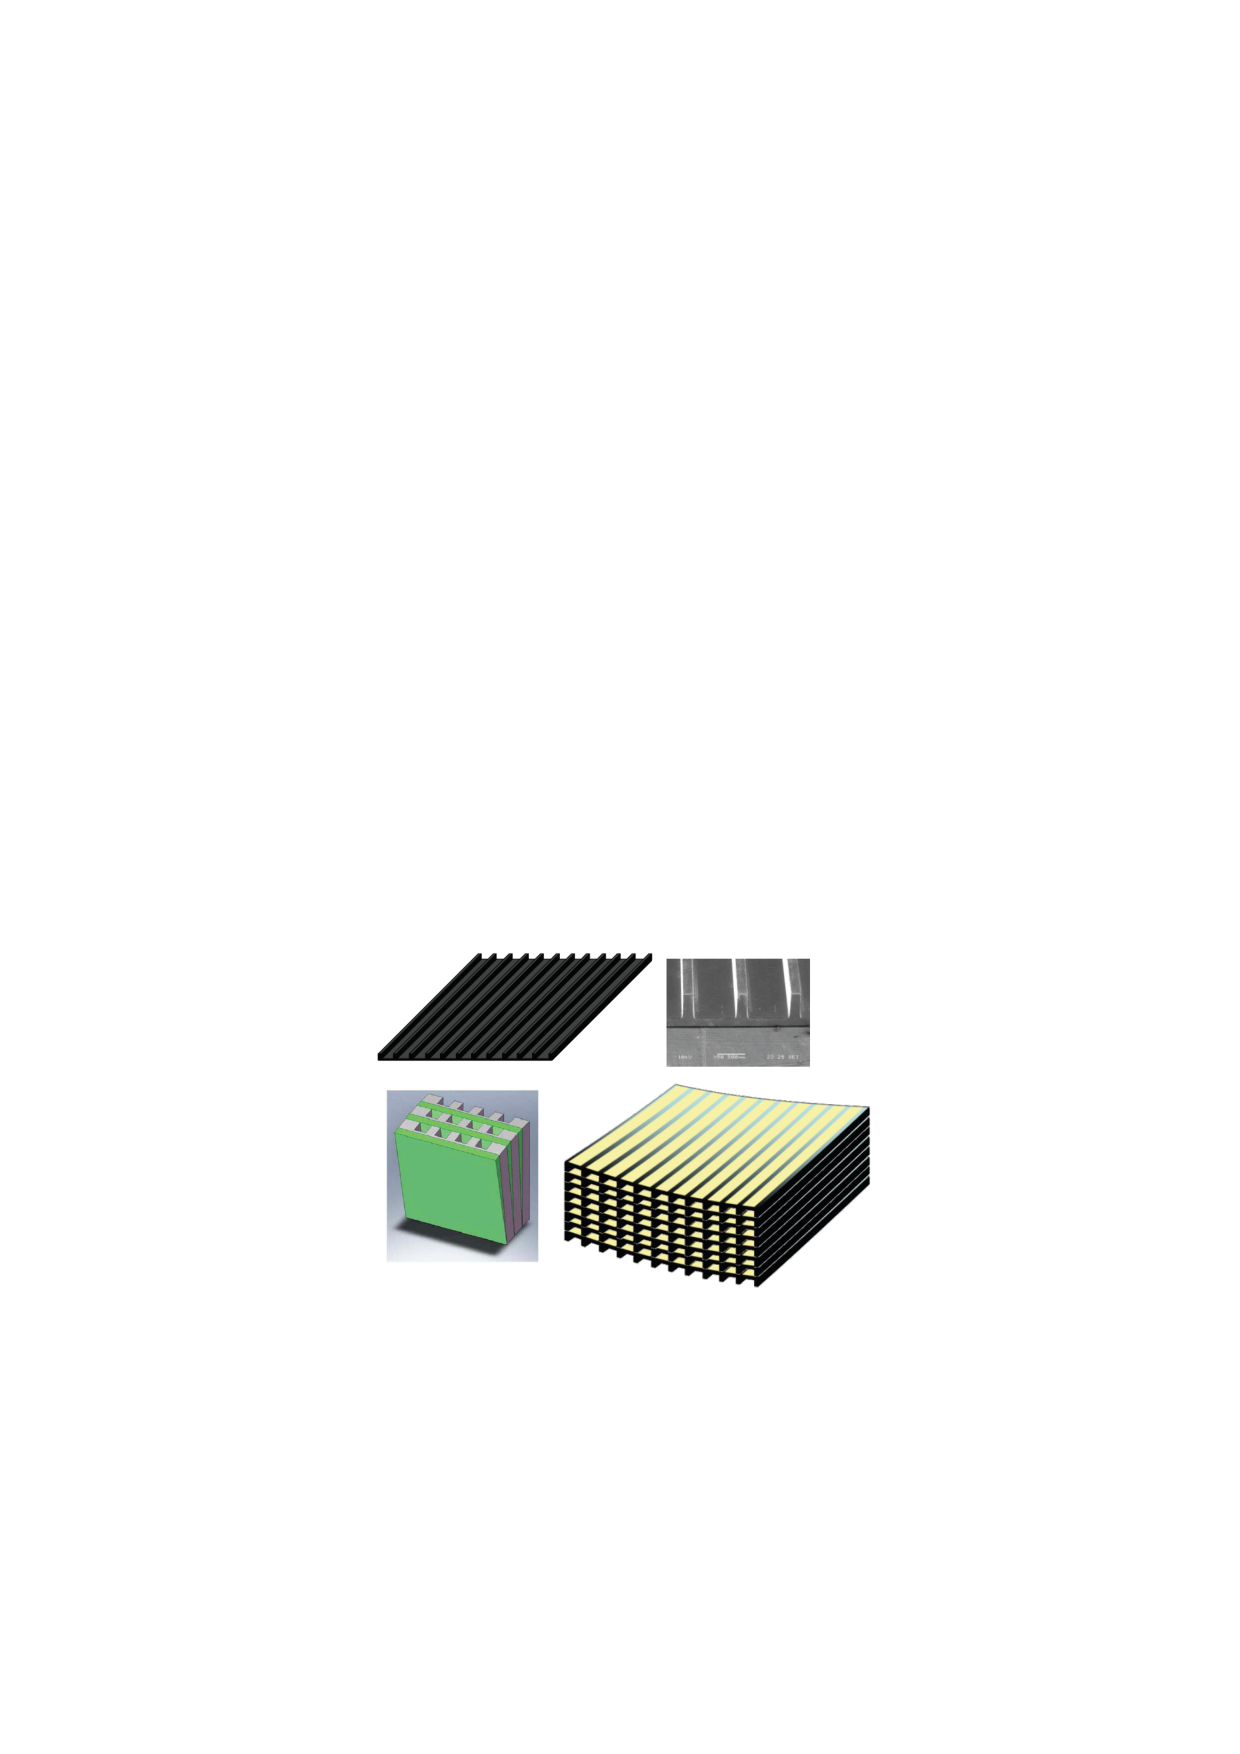
\includegraphics[width=\linewidth]{figures/athena/spo_principle1.pdf}
%   \captionof{figure}{\footnotesize  (from \cite{Willingale:2013vo}).}
%   \label{fig:spo_principle1}
% \end{minipage}%
% \hspace{20pt}
% \begin{minipage}{.47\textwidth}
%   \centering  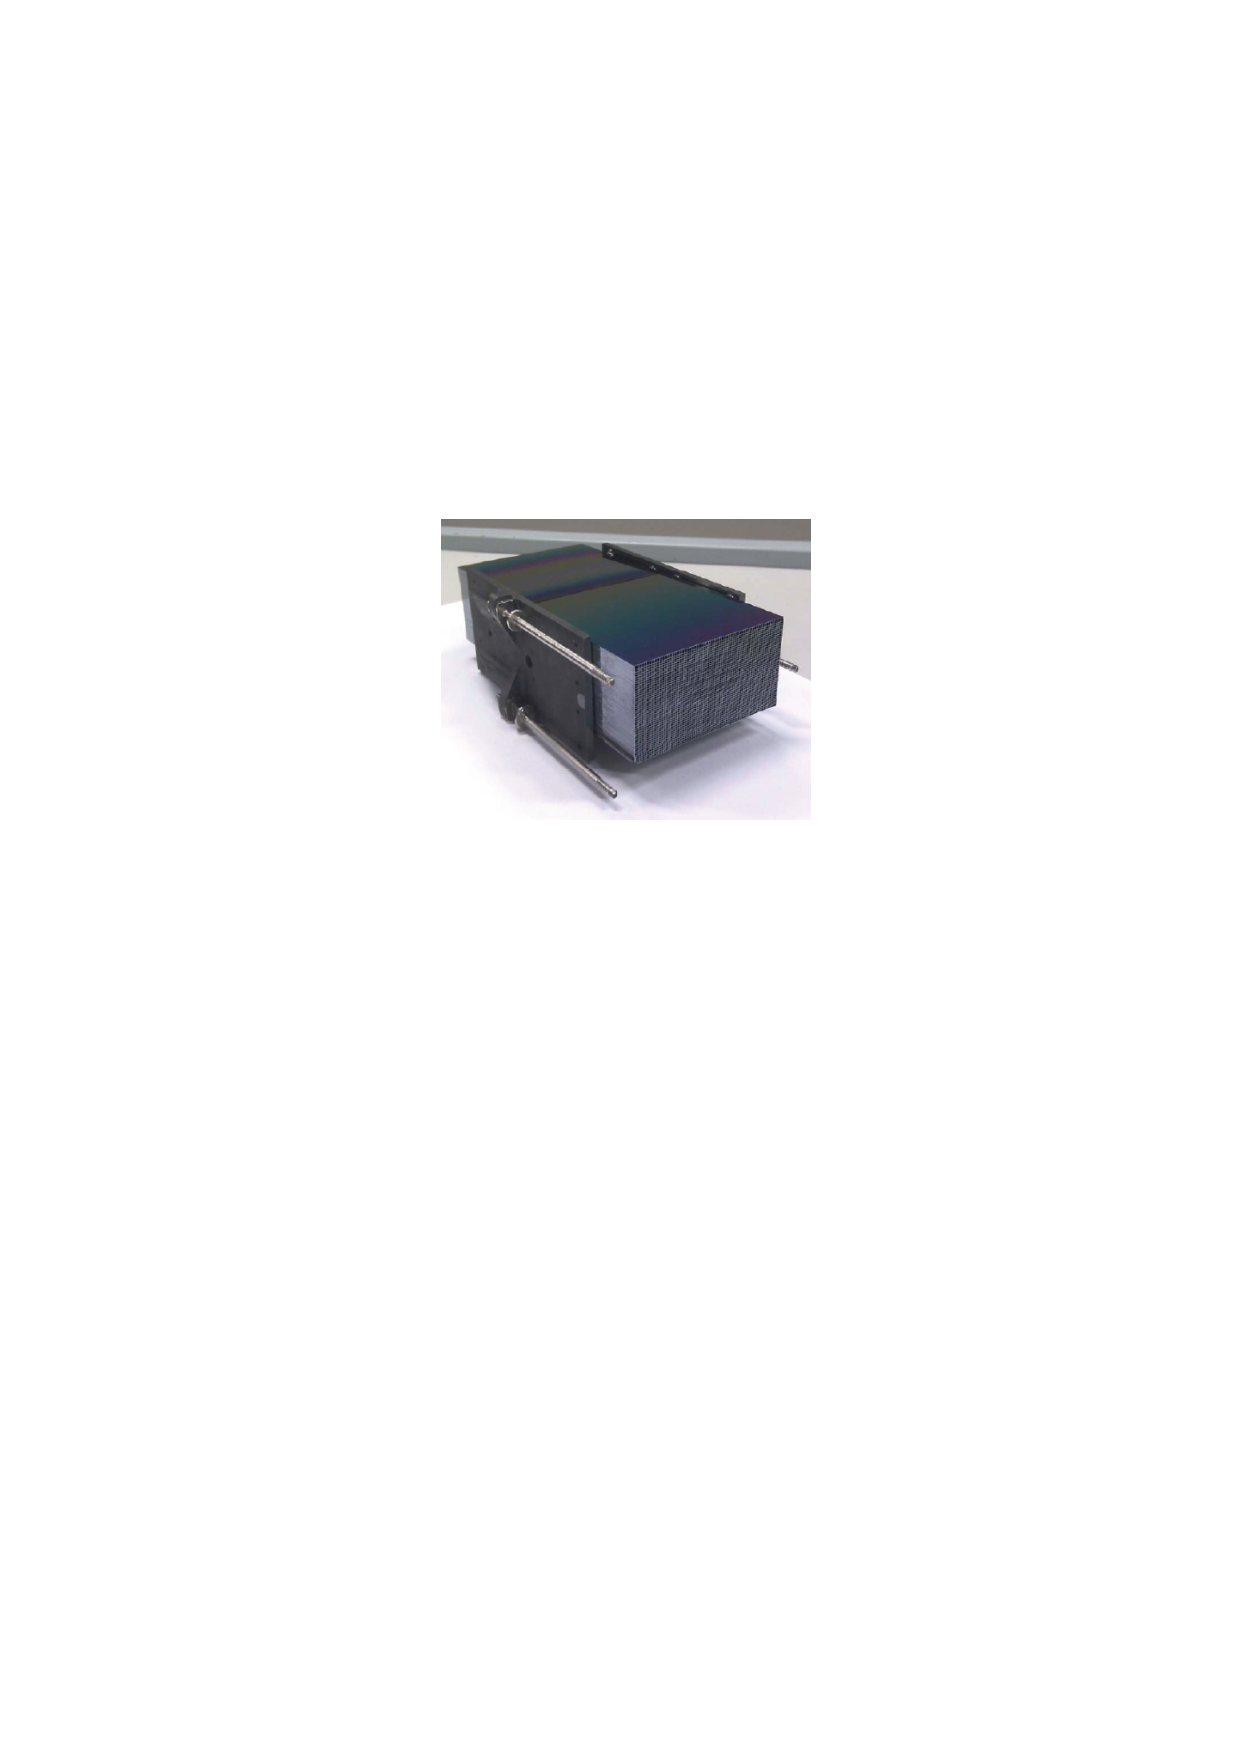
\includegraphics[width=\linewidth]{figures/athena/spo_stack.pdf}
%   \captionof{figure}{\footnotesize }
%   \label{fig:spo_stack}
% \end{minipage}
% \end{figure}

The silicon wafers are diced, wedged and grooves are cut into the underside, see figure \ref{fig:spo_principle1}. The grooves are 0.83 mm wide and spaced only 0.17 mm apart, resulting in narrow ribs in the underside. The grooving has two purposes: First, the wafer becomes so thin that it is bendable transversely to the ribs. Second, the SPO substrates can be stacked directly on top of one another with the ribs bonding to the surface of the substrate underneath. The X-rays will the be able to pass between the ribs and reflect on the surface of the bottom substrate. Stacking 68 of the SPO wafer substrates results in a very light, but very rigid block of silicon with micro-pores and a reflecting surface inside each pore. In order to have the SPOs reflect photons to the same spot, a wedge is applied to each reflecting surface corresponding to the angle required, see figure \ref{fig:spo_principle1} bottom left. The wedge is made from SiO$_x$ that is etched to the correct thickness and slope.

As the SPO substrates can be bend, they are stacked on a mandrel with the exact curvature needed. The high-precision stacking process is done by a dedicated robot in a controlled ultra-clean environment, as single dust specks can offset the stacking precision.

Two stacks of 68 SPO substrates constitutes an SPO module as can be seen in figure \ref{fig:spo_stack}. Each stack will reflect an incoming X-ray photon once, so two stacks acts like a conical approximation to the double-reflection Wolter I optic. However, in order to achieve sub-10'' angular resolution as specified by the science-criteria for ESA, the SPO technology will need to achieve a true Wolter I shape. Several initiatives by ESA are underway to achieve this as of 2014.

\begin{figure}[!h]
  \center
  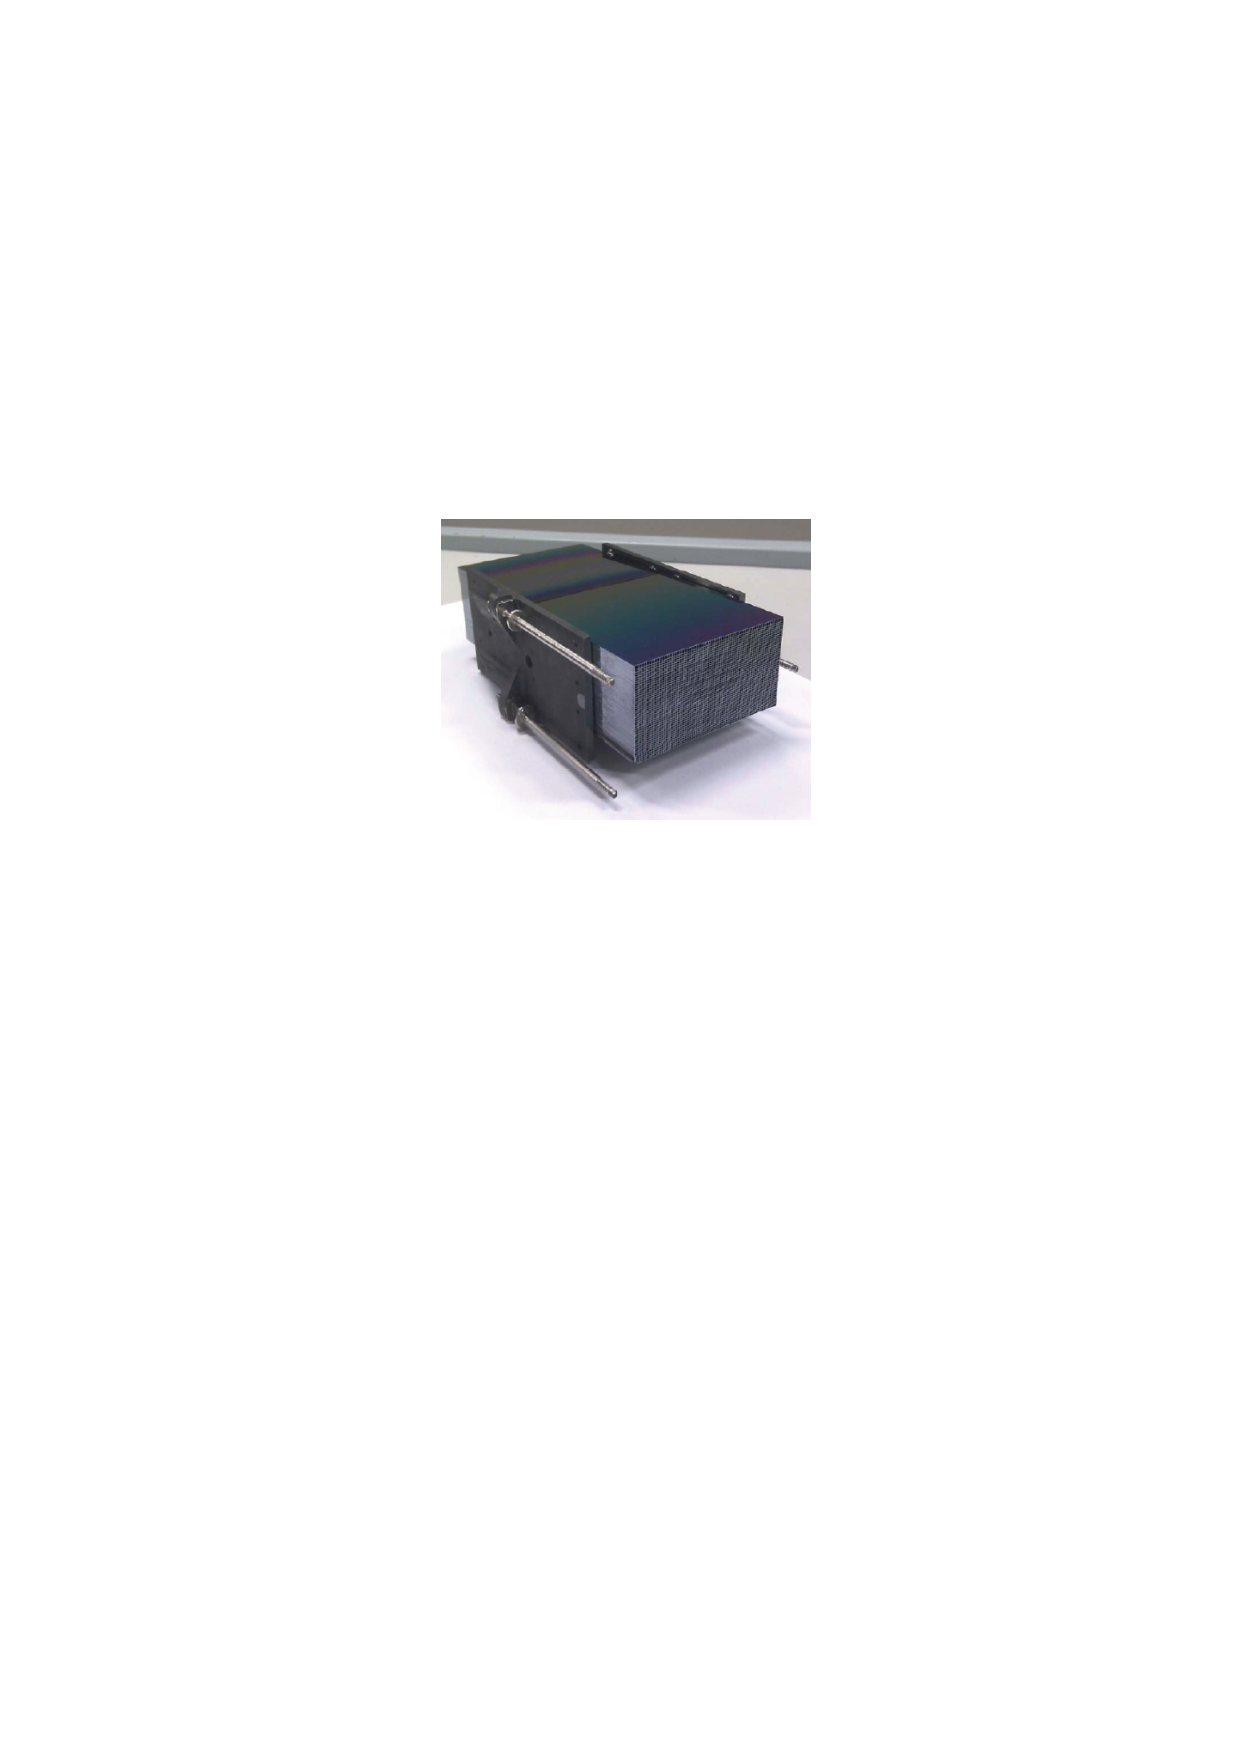
\includegraphics[height=7cm]{figures/athena/spo_stack.pdf}
\caption{\footnotesize A complete SPO mirror module. Two stacks of 68 SPO substrates are glued together with a pair of Cesis plates, making them co-aligned with 1'' precision. The complete module reflects an incoming X-ray photon twice and thus acts as both paraboloid and hyperboloid of the Wolter I optic. (from \cite{Willingale:2013vo}).}\label{fig:spo_stack}
\end{figure}

Each SPO module is self-consistent, making the entire optic technology modular. When a module is ready, it can be slided into a light-weight construction. This is in contrast to the NuSTAR technology (see section \ref{sec:nustar}) where each layer had to be mounted sequentially. The modularity is also a necessity when it becomes apparent that an effective area of 2 m$^2$ at 1 keV requires 1.5 mil. pores. As Athena is a large ESA mission, the Ariane V rocket will be used and the telescope is designed with the size limitations of the Ariane V fairing in mind, resulting in a telescope with $\sim$3 m diameter and $\sim$13 m length. To populate an optic with a diameter of $\sim$3 m, the number of SPO modules needed are $\sim$1,090 as can be seen in figure \ref{fig:Athena_full_optic}.

\begin{figure}[!h]
  \center
  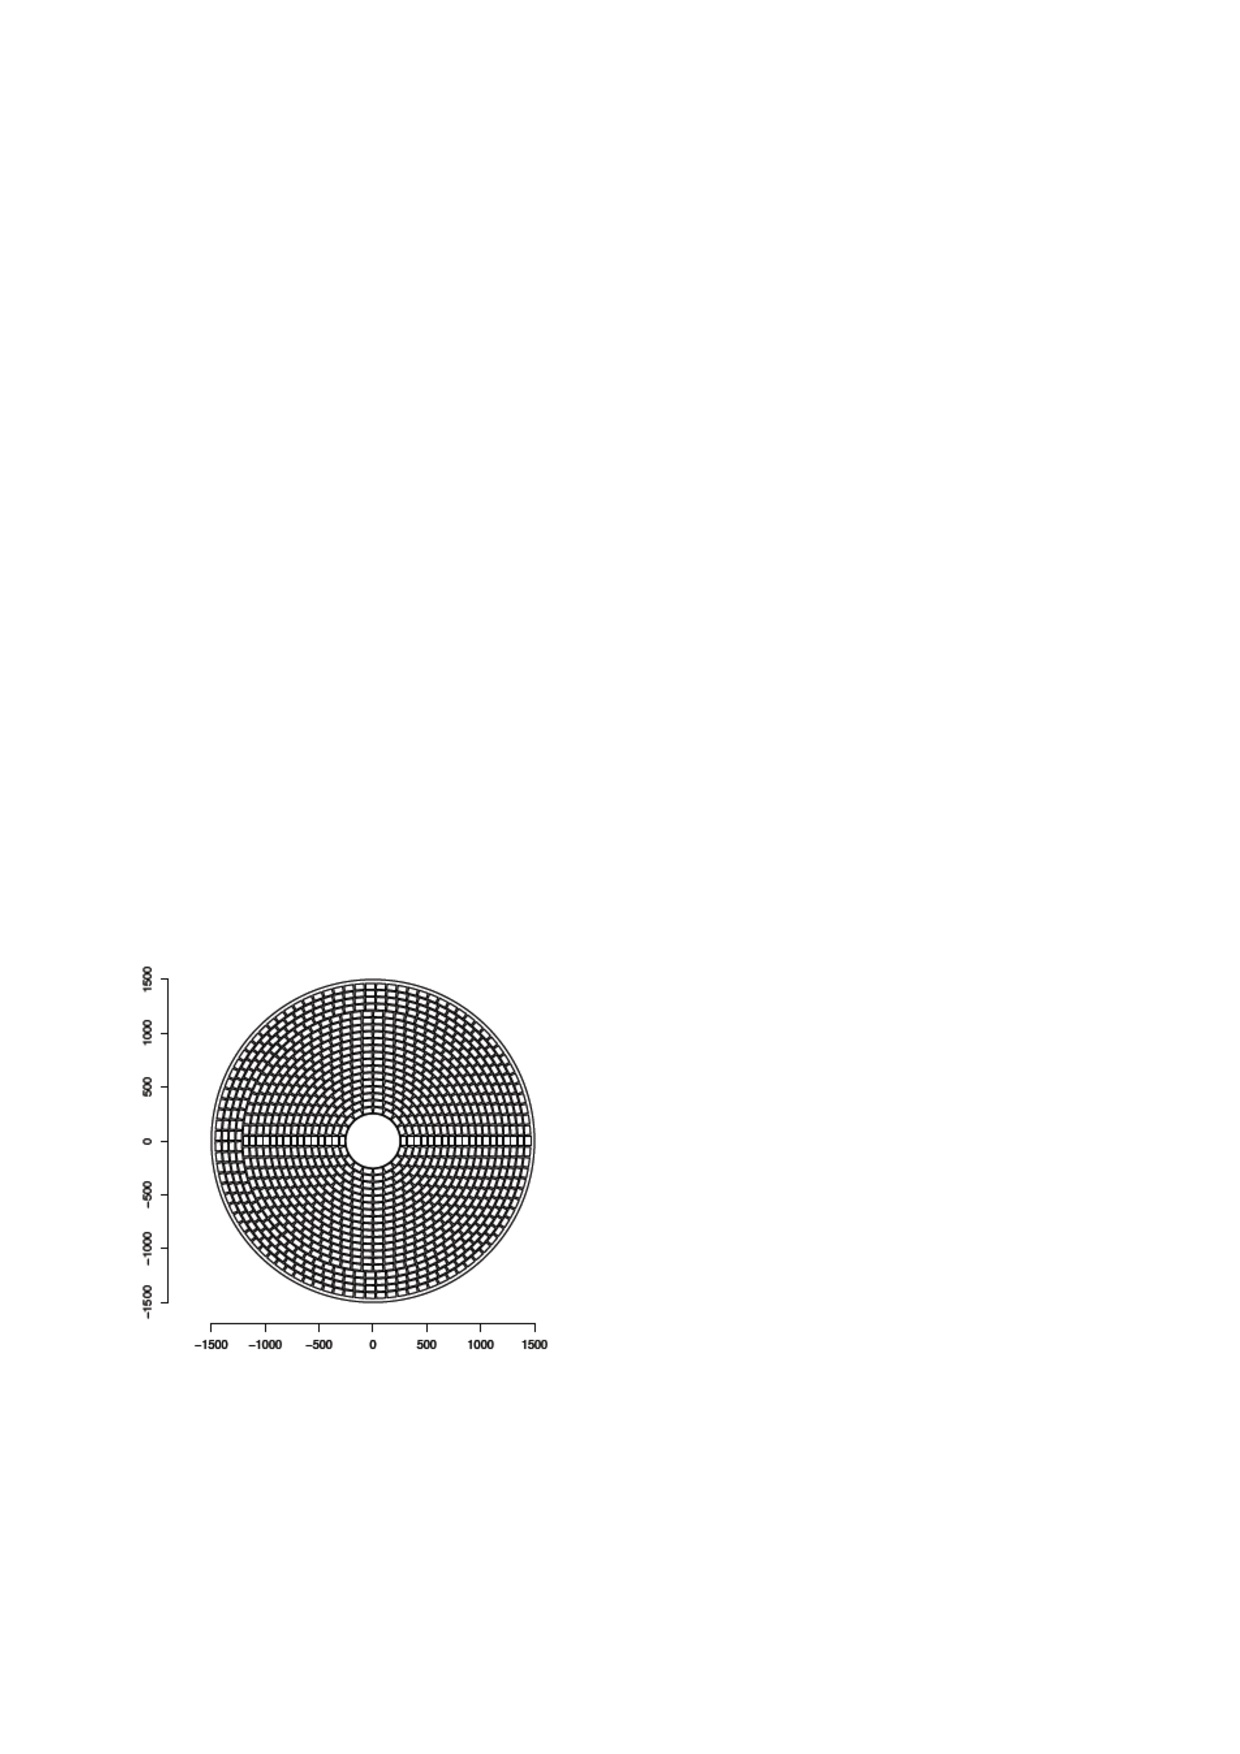
\includegraphics[height=7cm]{figures/athena/athena_full_optic.pdf}
\caption{\footnotesize The complete Athena optic. SPO mirror modules are arranged in rings to populate the aperture. (from \cite{Willingale:2013vo}).}\label{fig:Athena_full_optic}
\end{figure}

As each optic module consist of $2 \cdot 68 = 136$ SPO substrates, a total of $1090 \cdot 136 \approx 140,000$ SPO substrates are needed, not accounting for spares or broken substrates. Considering that the NuSTAR telescope consisted of $2\cdot2376$ glass substrates and took two years to produce, it becomes apparent that the Athena mission will require a large-scale production facility. In section \ref{sec:Athena_upscaled} can be found an investigation in the coating side of the production facility requirements for the Athena mission.

\subsection{Reflective coatings on SPO substrates}\label{sec:litho_process}
One of the most important principles of the SPO technology is the ability for the SPO substrates to bond when stacked. It is achieved by pressing the surface of one SPO substrate against the ribs of another SPO substrate. Since the SPO substrates are wedged with a SiO$_x$ material, both ribs and surface consist of SiO$_x$ and pressing the two substrates together forms a strong covalent bond, thereby fusing the two.

In order to apply a reflective coating to each of the SPO substrates, the bonding process has to be taken into account. Applying a coating with a physical vapor deposition process such as DC magnetron sputtering will coat the whole surface, but by using a lithographic process from the semiconductor industry it is possible to apply coatings in patterns on a surface. The pattern being the exact position where the ribs will touch the surface when stacking, so these areas are $\sim$0.17 mm wide, covers the entire length of the substrate surface and are spaced $\sim$0.83 mm apart. The lithographic process involves the following (also seen in figure \ref{fig:litho_process}):

\begin{itemize}
  \item Applying a resist film on the substrate surface.
  \item Curing the resist with e.g. a UV light in a striped pattern corresponding to the ribs of the SPO substrate.
  \item Removing the un-cured resist with a chemical solution (the developer).
  \item Coating the substrate with a reflective coating.
  \item Removing the cured resist including the coating applied on top of the resist using acetone or dimethyl sulfoxide (DMSO).
\end{itemize}

\begin{figure}[!h]
  \center
  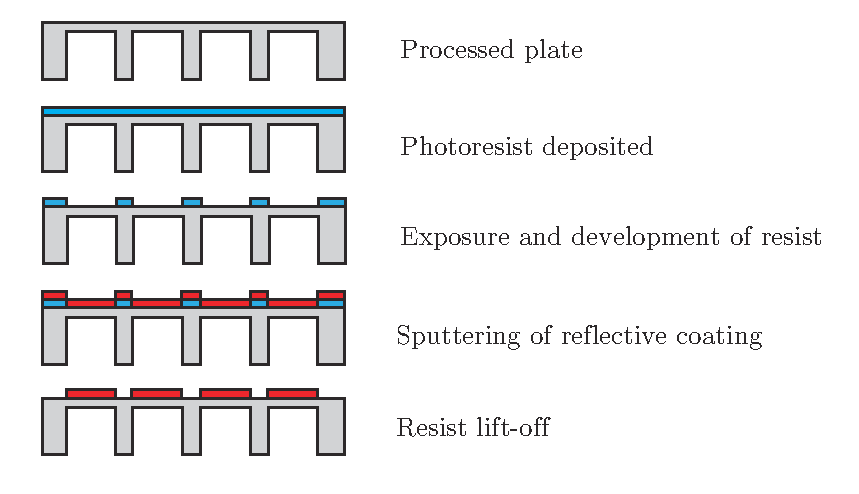
\includegraphics[height=8cm]{figures/athena/litho_process.pdf}
\caption{\footnotesize. The lithographic process applied to SPO substrates to achieve a striped pattern of reflective coating.}\label{fig:litho_process}
\end{figure}

The lithographic process puts requirements on the reflective coatings applied to the SPO substrates since chemical solutions used in the last step are designed to break carbon-carbon bonds. All multilayer coatings with pure C as the low-Z material are excluded as the last step described above will simply break apart the coating.


\section{Film stress from Ir/B$_4$C coatings}\label{sec:Athena_cr_impro}
The baseline coating for Athena consists of a bilayer of Ir and B$_4$C, the former of which shows considerably film stress of up to $\sim$-4 GPa (compressive). High film stress of more than 1 GPa can in films cause deadhesion and "hillocks" on the surface of films with compressive stress. Some bending of the coated substrate will also result from high stress, the degree depending on substrate thickness.

To alleviate the stress in the film, earlier investigations has shown significant improvements in stress by using a Cr underlayer, which almost eliminates the total film stress[\ref{pap:PREL_Athena}]. The drawback of using Cr films is the high surface roughness, with r.m.s roughness of 0.1--1.0 nm normal for a 10 nm thick film. The following section investigates possible improvements to that roughness.

\subsection{Improving roughness in stress-relieving Cr sublayers}
We present here the results of two experiments with the purpose of reducing the Cr surface roughness. The first experiment is an attempt to decrease the rate of sputtered Cr atoms reaching the substrate. A lower rate will give an adsorbed Cr atom a chance to move to a lower position\cite{Venables:1984wu}. By decreasing the output power to the Cr cathode, while maintaining the same voltage of -400 V, the rate of sputtered atoms can be decreased. In figure \ref{fig:cr-power-change} XRR measurements of Cr films coated at varying power output can be seen.

\begin{figure}[!h]
	\center
	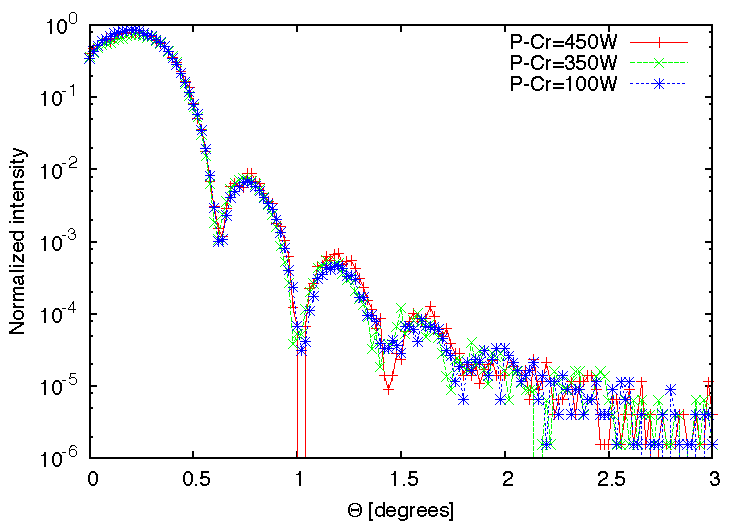
\includegraphics[height=8cm]{figures/athena/coatings/cr-power-change.pdf}
\caption{\footnotesize XRR measurements of four Cr single layer coatings made with varying power settings.}\label{fig:cr-power-change}
\end{figure}

It is seen that at lower power settings, the hills and fringes become less pronounced, indicating a higher roughness. This would indicate that the flux of sputtered atoms adhering to the substrate have time to coalesce into islands, thereby giving rise to island-growth also known as \emph{Volmer-Weber} growth\cite{Thompson:2000ge}. In that case, it would seem that lowering the power on Cr yields a higher surface roughness because given enough time, the Cr adatoms will form into their preferred configuration.

A second experiment involves changing the Ar gas pressure during coating. A minimum pressure is required in order to sustain the cathode plasma, but it is beneficial to coat at the lowest possible pressure. At a given pressure, the sputtered atoms going from target to substrate will have a chance of hitting an Ar atom given by the mean free path. A sputtered atom that would otherwise hit the substrate at a very low normal angle, will after having hit an Ar atom reach the substrate at a much higher angle, thereby giving rise to shadow-effects\cite{Barabasi:XbjHWFWZ} as seen in figure \ref{fig:self-shadow}.

\begin{figure}[!h]
	\center
	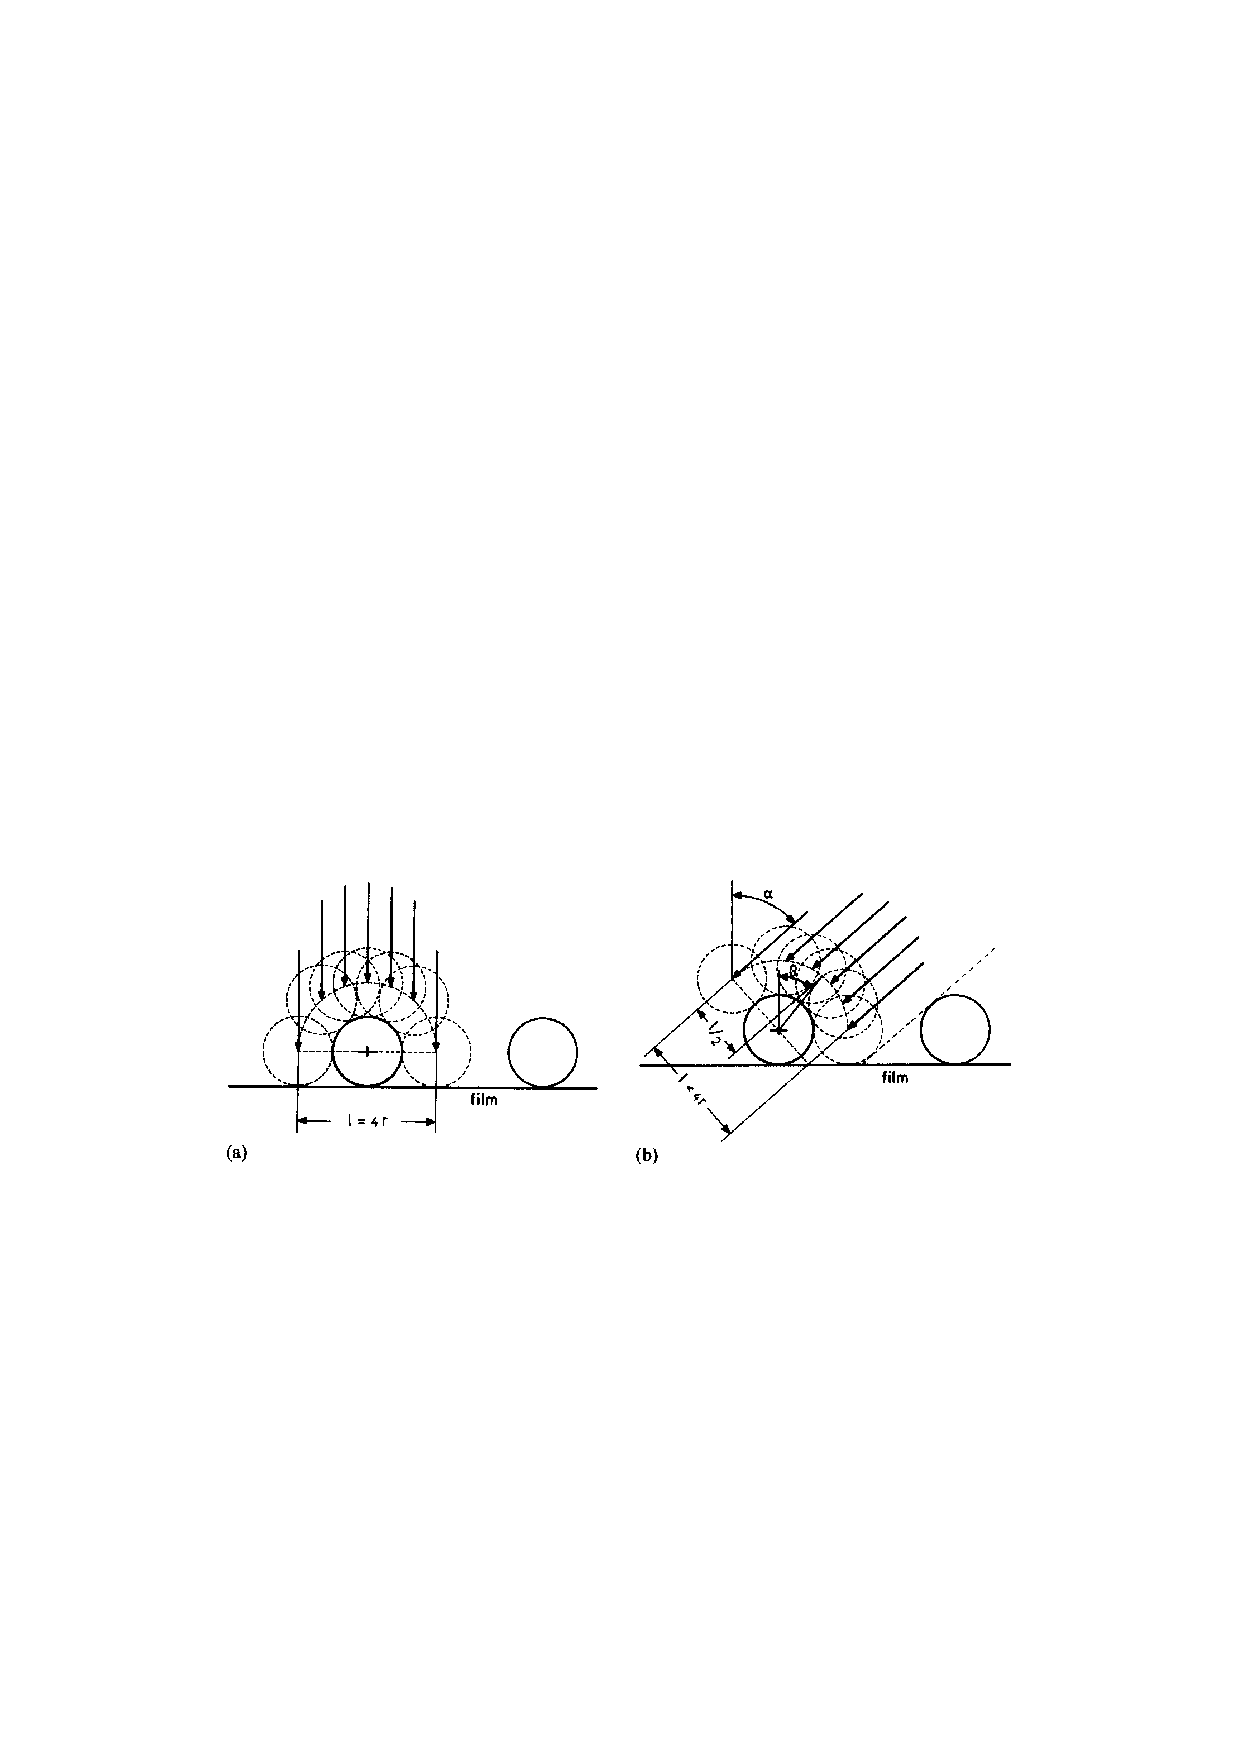
\includegraphics[height=5.5cm]{figures/athena/coatings/self-shadow.pdf}
\caption{\footnotesize Principle of self-shadowing during angled deposition on a surface. At higher angles, incoming particles will have a tendency to adsorb on top of single particles already on the surface instead of filling gaps in the film. From \cite{Dirks:1977uk}.}\label{fig:self-shadow}
\end{figure}

By producing Cr coatings at varying Ar pressures and measuring using XRR, a correlation was found between Ar pressure and Cr surface roughness. The XRR measurements along with IMD fits can be seen in figure \ref{fig:cr-pressure-fit}. A decrease in Cr surface roughness from 1.0 nm to 0.7 nm is seen when going from 2.4 mTorr to 1.5 mTorr Ar pressure.

\begin{figure}[!h]
	\center
	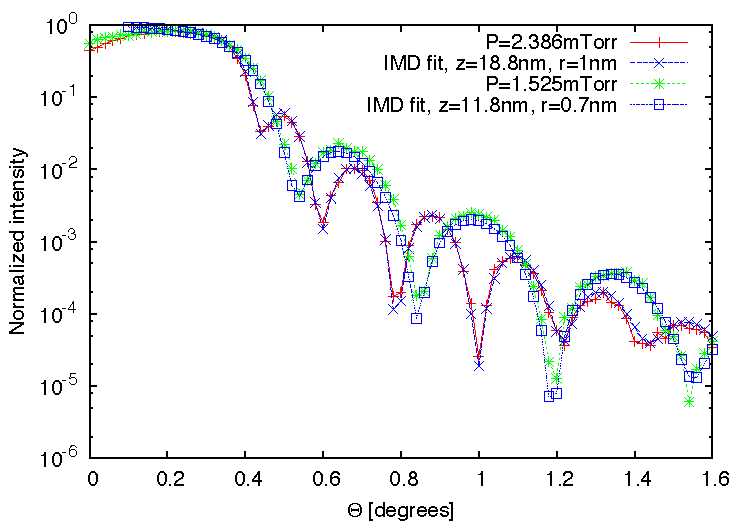
\includegraphics[height=8cm]{figures/athena/coatings/cr-pressure-fit.pdf}
\caption{\footnotesize XRR measurements of two Cr single layer coatings made with varying Ar pressure. Blue points are IMD models fitted to the data.}\label{fig:cr-pressure-fit}
\end{figure}

Earlier investigations of the baseline Ir/B$_4$C coating with Cr sublayer\cite{Jakobsen:2011vd} have hinted that the interface roughness of Ir/B$_4$C becomes lower than the interface roughness of Cr/Ir. A simple bilayer coating of Cr/Ir have now been made, where B$_4$C can be factored out of the fitting procedure. The B$_4$C has been left out, so to easier constrain the surface roughness of Ir and Cr in the fitting process as the model only has 4 variables compared to 6 variables for a Cr/Ir/B$_4$C coating. The coating was made using the standard Ar pressure of 2.9 mTorr. XRR measurement of the sample can be seen in figure \ref{fig:cr-ir-fit} along with a an IMD fit. The fitted curve shows a Cr/Ir interface roughness of 0.62 nm and an Ir surface roughness of 0.3 nm.
This is an extremely promising result, since the baseline Athena coating depends on the Ir surface for most of the energy response above $\sim$3 keV. So to have this surface smooth while at the same time keeping a low amount of film stress is reassuring.

\begin{figure}[!h]
	\center
	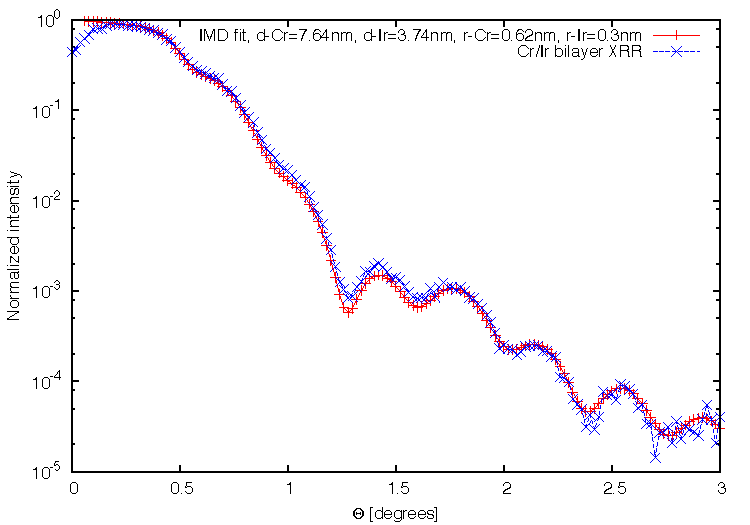
\includegraphics[height=8cm]{figures/athena/coatings/cr-ir-fit.pdf}
\caption{\footnotesize XRR measurement of a bilayer of Cr/Ir (red) along with an IMD model fitted to the data (blue).}\label{fig:cr-ir-fit}
\end{figure}

\section{Investigation of pulsed-DC sputtering}
We investigated the use of pulsed sputtering to decrease roughness as thickness increase as described in the litterature\cite{Pei:2009gn,Shaha:2011gy,Turkin:2010ur}. In the paper by Pei et al, a sputtering cathode with a C target was supplied with -400 V and 1.5 A at 350 kHz and 50\% duty cycle. The substrate was place 10 cm away from the target and supplied with -40 V at 250 kHz at 50 \% duty cycle. The high frequency at the target allows for a much higher percentage of the sputtered atoms to become ionized, giving them a positive charge. At regular non-pulsed DC sputtering, only 10 \% are ionized atoms, but for pulsed that increases to 60-70 \%\cite{Bradley:2002ge,Pei:2008jl}. The negative pulsed bias on the substrate will pull in the ionized sputtered atoms at much higher velocity than possible for DC sputtering. The higher velocity sputtered atoms gives rise to denser and more smooth films, as the momentum of the impact causes a temporary \emph{liquification} of the immediate surrounding thin film on the nano-scale.

Attempts by Pei et al show promising results for decreasing interlayer roughness in multilayers using a high frequency pulse modulation on the power delivered to the cathode with lighter material, in their case carbon was used. For coatings for the Athena mission, it is critical to use B$_4$C as the light material, as a regular C layer will be dissolved in the lift-off process that removes the lithographic resist.

We acquired the same power supply, an Advanced Energy Pinnacle Plus+ 5+5 capable of delivering two channels of 5 kW at 350 kHz. Using W and B$_4$C, 10 bilayer coatings were produced with the same power supply setup as mentioned in \cite{Pei:2009gn}. The entire rotating ring in the multilayer coating chamber at DTU Space is designed to hold a separate bias or be grounded depending on configuration. Initial results can be seen in fig. \ref{fig:wb4c-pulsed}.

\begin{figure}[!h]
	\center
	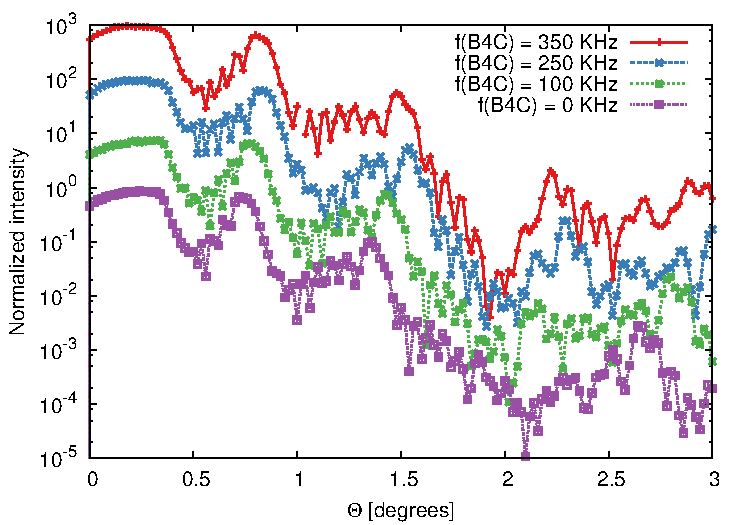
\includegraphics[height=8cm]{figures/athena/coatings/w-b4c_pulsed_2.pdf}
\caption{\footnotesize XRR measurements of four W/B$_4$C 10 bilayer films made with varying pulsed-DC frequency on the B$_4$C cathode. Note: Measurement data shifted vertically to be easier to distinguish.}\label{fig:wb4c-pulsed}
\end{figure}

The figure show XRR measurements of 4 samples coated with 10 bilayer W/B$_4$C with different frequencies supplied to the B$_4$C target. For a 10 bilayer coating, we expect to see clear Bragg peaks with 8 Kiessig\cite{Kiessig:1931vo} fringes between, but all samples show washed out 1st and 2nd order Bragg peaks and an indeterminate number of Kiessig fringes. Even the sample coated without a pulsed B$_4$C cathode show the same behavior. In figure \ref{fig:wb4c-nopulsed}, the two samples coated with 350 kHz and 0 kHz in the same coating run is compared to a sample from a different run coated with regular DC sputtering showing well-defined Bragg peaks as would be expected.

\begin{figure}[!h]
	\center
	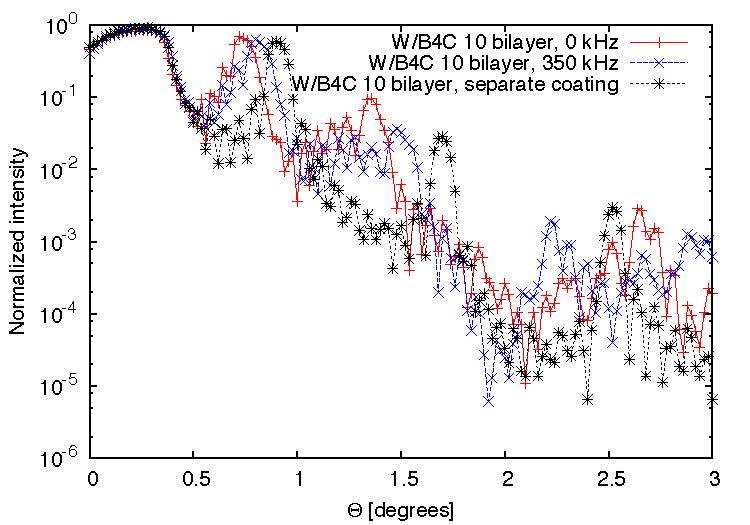
\includegraphics[height=8cm]{figures/athena/coatings/w-b4c-nopulsed.pdf}
\caption{\footnotesize XRR measurements of three W/B$_4$C 10 bilayer films. Two (red and blue) made using pulsed-DC sputtering and also shown in figure \ref{fig:wb4c-pulsed}. The last one (black) is made in a separate coating run without pulsed-DC sputtering, but otherwise with the same coating parameters.}\label{fig:wb4c-nopulsed}
\end{figure}

Something has clearly gone wrong in the pulsed-DC coating. The new software recently installed to control the multilayer coating chamber logs the cathode output every 5 seconds and a plot of that can be seen in figure \ref{fig:power-output}(left) compared to a log from a regular DC coating, figure \ref{fig:power-output}(right). The figure shows clearly that the power output to the B$_4$C cathode drops to zero in the middle of a rotation. The B$_4$C cathode should be at 900 W output for the entire time the W cathode is off.

\begin{figure}[!h]
	\center
	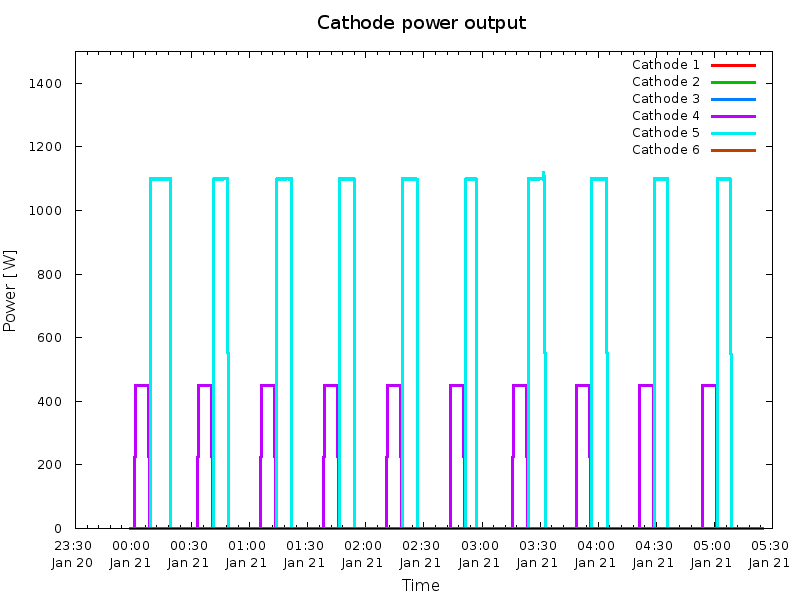
\includegraphics[width=0.47\linewidth]{figures/athena/coatings/power_output_rf_coating.png}
	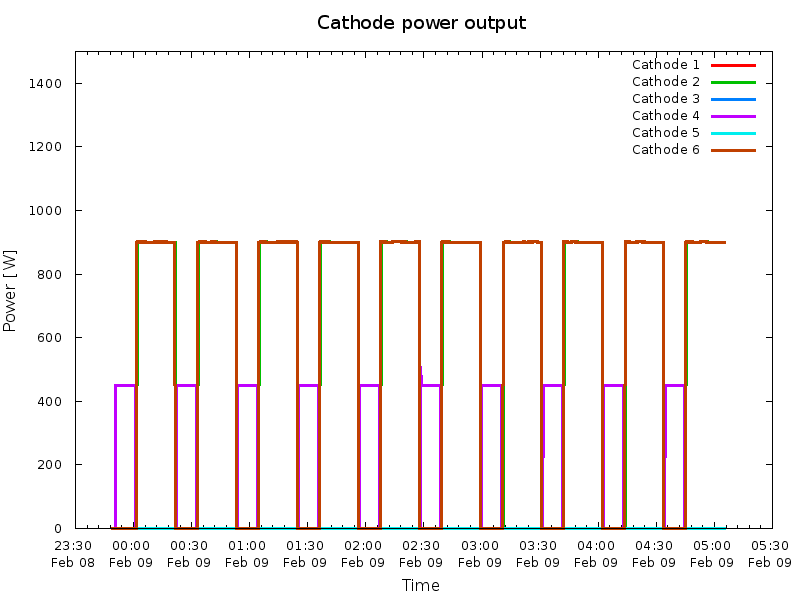
\includegraphics[width=0.47\linewidth]{figures/athena/coatings/power_output_dc_coating.png}
\caption{\footnotesize Graphs of cathode power output over time during a coating run. Left is from a W/B$_4$C 10 bilayer coated using pulsed-DC sputtering on the B$_4$C material. Right is from a W/B$_4$C 10 bilayer coating made without pulsed-DC sputtering.}\label{fig:power-output}
\end{figure}

It is not uncommon to see a cathode 'drop out' during a coating run, where the power supply is unable to sustain the plasma. In that case the power supply will increase the voltage to get the plasma to ignite again and the power output will in that period be 30-40 W. In this case the power output drops to zero, which is inconsistent with a conventional drop-out. Investigating the matter further shows that the 'arc'-protection system on the power supply goes off rapidly during a coating. Arcs are a sudden discharge from cathode to the grounded anode shield and can have a wide variety of causes. The arc-protection will protect the power supply from the power surge and will tell the user when it happens. The inner anode shield in the B$_4$C cathode clearly shows damage from arcing in the steel and the shielding teflon strips, which looks like welding marks. We assume that at some point during the coating, the damage creates enough debris to make a short between cathode and anode shield.

It is at this moment still unclear what causes the arcing. The pulsed-DC system brings many more variables into an already complicated sputtering process. The best assumption at the moment is either that the cables from power supply to cathode are too long or that a wire assembly box has insufficient electrical shielding.

\begin{figure}[!h]
	\center
	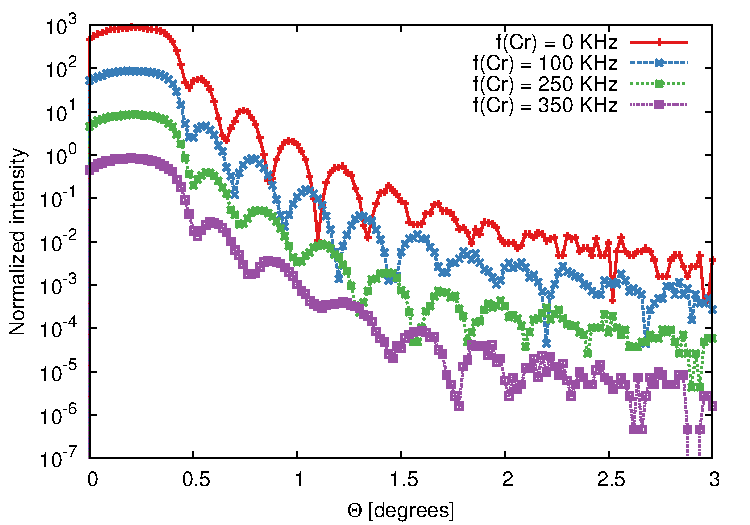
\includegraphics[height=9.5cm]{figures/athena/coatings/cr_pulsed_2.pdf}
\caption{\footnotesize XRR measurements of four samples coated with single layers of Cr using pulsed-DC sputtering at varying frequency. Sample coated with $f=0$ kHz (red) has a thickness of $\sim$17 nm. Sample coated with $f=350$ kHz (purple) has a thickness of $\sim$12 nm. Note: Measurement data shifted vertically to be easier to distinguish.}\label{fig:cr-pulsed}
\end{figure}

The second attempt at using the pulsed-DC method was with Cr single layer coatings. XRR measurements of the coated samples can be seen in figure \ref{fig:cr-pulsed}. Four samples were coated with varying frequencies applied to the Cr cathode. The measurements show clear differences in coated thickness between the frequencies used (position of Kiessig fringes does not overlap) and higher frequencies show a lower surface roughness (Kiessig fringes are less pronounced and shows a wavy pattern at the highest frequency). The XRR measurements were difficult to fit using IMD, indicating that the films are of non-uniform density. The coating done without pulsed-DC fitted to a $\sim$17 nm Cr thickness and the coating done with the highest frequency pulsed-DC sputtering fitted to a $\sim$13 nm Cr thickness. No arcing was seen when coating Cr using pulsed-DC sputtering.

We believe that the investigation of pulsed-DC sputtering have concluded with no improvements in the coatings. The arcing that was seen during pulsed-DC sputtering of B$_4$C, but did not show up for Cr, can have a variety of causes. First, the output power when coating B$_4$C is significantly higher than for Cr (1100 W compared to 450 W). The higher power puts higher demand on electrical shielding as well as the cable length between power supply and cathode. Second, there are fundamental differences in the two materials. The Cr is a well conducting and hard metal, whereas B$_4$C is not very well conducting and brittle. A very good contact is required between cathode and sputter material, but since the B$_4$C is very stiff and not as malleable as metal, the target can easily crack which will give rise to areas of non-contact. In conclusion, the whole process is not well understood, but has potential as seen in the literature.

\section{Reactive sputtering of W/B$_4$C with N$_2$}
Improving interlayer roughness of multilayer coatings using N$_2$ reactive deposition has been shown before\cite{Windt:2007uj,jakobsen2010developing}, specifically for W/B$_4$C films. For this project, coatings of 10 bilayer W/B$_4$C were produced using N$_2$ reactive sputter deposition and compared to similar coatings made without N$_2$. XRR measurements of the results and comparison can be seen in figure \ref{fig:wb4c-n2}. The right figure show coatings with a d-spacing of $\sim$3.5 nm, and the left coatings with d-spacings of $\sim$5.0 nm. The right figure show a horizontal offset in the XRR measurement between the two coatings, contributed by an offset in the calibration. The left figure show a similar offset, but also a significant change in Kiessig fringe intensity between the 2nd and 3rd Bragg peak. The 3rd Bragg peak is also less pronounced for the reactively sputtered film than the non-reactively sputtered. The results indicate that the reactive sputtering does not improve the interface roughness, but rather increases interlayer roughness.

\begin{figure}[!h]
	\center
  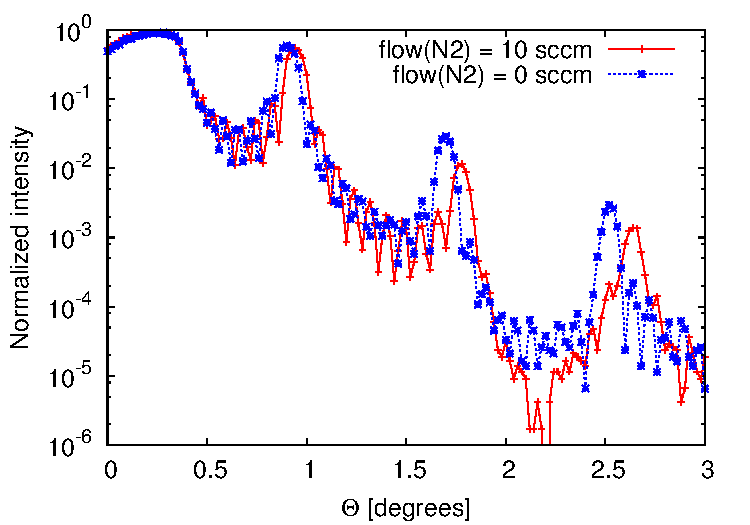
\includegraphics[width=0.47\linewidth]{figures/athena/coatings/w-b4c_n2_50AA.pdf}	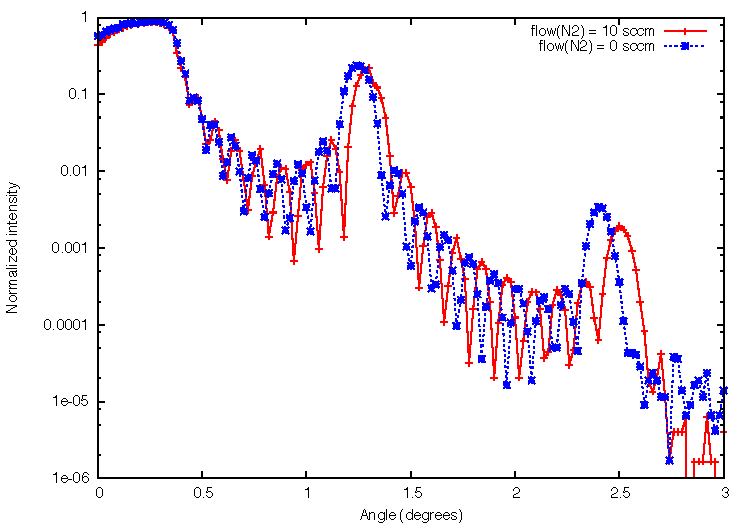
\includegraphics[width=0.47\linewidth]{figures/athena/coatings/w-b4c_n2_35AA.pdf}
\caption{\footnotesize XRR measurements of 10 bilayer W/B$_4$C coatings made with and without N$_2$ reactive sputtering (10 \% N$_2$, 90 \% Ar).  \textbf{Left:} Coatings with a d-spacing of $\sim$5 \textbf{Right:} Coatings with a d-spacing of $\sim$3.5 nm. nm.}\label{fig:wb4c-n2}
\end{figure}

It was later found out from samples stored over a longer period, that the coatings will visibly change over time if coated with N$_2$ reactive sputtering. A sample with discoloration can be seen in figure \ref{fig:discolor} (picture taken July 2014). The sample is a W/B$_4$C 10 bilayer calibration coating with a d-spacing of $\sim$5 nm. It was coated in February 2012 using 10 \% N$_2$ with 90 \% Ar at a total pressure of 2.9 mTorr.

\begin{figure}[!h]
	\center	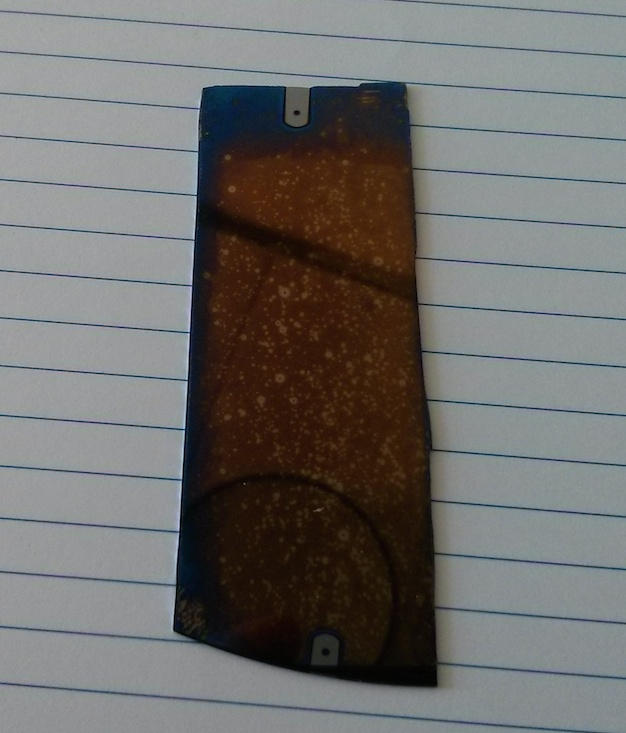
\includegraphics[height=9cm]{figures/athena/coatings/si5556.jpg}
\caption{\footnotesize Picture of Si wafer sample coated with 10 bilayers of W/B$_4$C using N$_2$ reactive sputtering. Sample was coated in February 2012, picture taken July 2014. The surface over time turned a yellow/brown colour with the edges black/blue. Top and bottom are marks from the clips holding the sample in place during coating. The clear uncoated surface is visible in those spots.}\label{fig:discolor}
\end{figure}

Investigation into the literature gives a possible explanation. B$_4$C coatings react to humidity, but for BN coatings the effect is even more pronounced. The coating will absorb water molecules from the air, which diffuses through the coating and can eventually make the film peel off\cite{Cardinale:1994ha}. When B$_4$C coatings are sputtered with N$_2$ present, the nitrogen atoms become part of the film and will form B-N bonds. That would make all B$_4$C films produced with N$_2$ reactive sputtering deteriorate at ambient humidity. To test the hypothesis, a number of samples were produced with and without reactive sputtering, measured with XRR and subsequently placed in a desiccator at $\sim$20\% humidity.

The results can be seen in figure \ref{fig:wb4c-n2-storage}. The upper row are thick ($\sim$5.0 nm) and thin ($\sim$3.5 nm) samples of 10 bilayer W/B$_4$C coated with 10 SCCM N$_2$ flow ($\sim$10\% N$_2$). Middle row are samples with the same type and thickness of coating, but without N$_2$. Bottom row are also coated without N$_2$ but placed at ambient humidity ($\sim$45\%) outside the desiccator. The bottom row are also only stored for 3 months. The reactively sputtered coatings in the upper row show little change from Feb. 4th to June 28th, $\sim$5 months. What is interesting is the center row that show some interfacial changes in the film, especially for the thicker sample (left figure). Comparing to the bottom row, the thicker sample does not show the same changes over the 3 month period, but the thinner sample show significant change. The critical angle has shifted or washed out, the Bragg peak has widened and lowered in intensity. The sample also show visible discoloration, which is something that was not expected of a coating made without N$_2$ reactive sputtering.

%A more in-depth investigation into this problem is reported in section \ref{sec:long_term}.

\begin{figure}[htbp]
	\center
  \footnotesize 	\begin{overpic}[width=0.47\linewidth]{figures/athena/coatings/w-b4c-n2-0sccm-thick.pdf}\put(35,40){Reactiv. sput. (10\% N$_2$)}
              \put(35,30){Stored in dessicator}\end{overpic}	\begin{overpic}[width=0.47\linewidth]{figures/athena/coatings/w-b4c-n2-0sccm-thin.pdf}\put(35,40){Reactiv. sput. (10\% N$_2$)}
              \put(35,30){Stored in dessicator}\end{overpic}	\begin{overpic}[width=0.47\linewidth]{figures/athena/coatings/w-b4c-n2-10sccm-thick.pdf}\put(35,40){Non-reactiv. sput.}
                \put(35,30){Stored in dessicator}\end{overpic}	\begin{overpic}[width=0.47\linewidth]{figures/athena/coatings/w-b4c-n2-10sccm-thin.pdf}\put(35,40){Non-reactiv. sput.}
                    \put(35,30){Stored in dessicator}\end{overpic}	\begin{overpic}[width=0.47\linewidth]{figures/athena/coatings/w-b4c-no-storage-thick.pdf}\put(35,40){Non-reactiv. sput.}
                    \put(35,30){Stored outside dessicator}\end{overpic}	\begin{overpic}[width=0.47\linewidth]{figures/athena/coatings/w-b4c-no-storage-thin.pdf}\put(35,40){Non-reactiv. sput.}
                \put(35,30){Stored outside dessicator}\end{overpic}

\caption{\footnotesize XRR measurements of samples coated with 10 bilayer W/B$_4$C films measured after coating and at a later time. Top and middle row samples were stored in a desiccator with $\sim$30 \% humidity. Bottom row samples were stored at ambient humidity ($\sim$50 \%).  \textbf{Top row} Samples coated with N$_2$ reactive sputtering (10 \% N$_2$, 90 \% Ar) and stored in desiccator, d-spacings of $\sim$5 nm (left) and $\sim$3.5 nm (right). \textbf{Center row} Samples coated with non-reactive sputtering and stored in desiccator, d-spacings of $\sim$5 nm (left) and $\sim$3.5 nm (right). \textbf{Bottom row} Samples coated with non-reactive sputtering and stored outside desiccator, d-spacings of $\sim$5 nm (left) and $\sim$3 nm (right) }\label{fig:wb4c-n2-storage}
\end{figure}

\subsection{W/B$_4$C coatings from long term storage}\label{sec:longterm_wb4c}
All samples coated at DTU Space are stored indefinitely for possible later investigation. The calibration samples of each material type for the Athena coatings are especially suitable for a long term investigation since the XRR measurement results of these samples have distinct features. In figure \ref{fig:longterm_wb4c} the results of XRR measurements of W/B$_4$C calibration samples are shown immediately after coating and after up to 18 months later. The samples are coated without N$_2$ and using the standard Ar pressure of 2.9 mTorr.

\begin{figure}[htbp]
  \center
  \footnotesize \begin{overpic}[width=0.47\linewidth]{figures/athena/coatings/w-b4c-kalib2.pdf}
\put(35,30){d $\sim$6 nm}\end{overpic}
\begin{overpic}[width=0.47\linewidth]{figures/athena/coatings/w-b4c-kalib1.pdf}
\put(35,30){d $\sim$3.5 nm}\end{overpic}
\caption{\footnotesize XRR measurements of coatings stored for 2-3 years at ambient conditions (outside desiccator). 10 bilayer W/B$_4$C with d-spacings of $\sim$6 nm (left) and $\sim$3.5 nm (right). }\label{fig:longterm_wb4c}
\end{figure}

The W/B$_4$C multilayers in  show significant change after less than two months. The thicker sample (left) have a shifted critical angle, corresponding to a change in $\Gamma$ in the multilayer. The thinner film (right) also show a change in critical angle, although less pronounced. The change in critical angle indicate either a change in $\Gamma$ in the multilayer or a change in density of either B$_4$C or W.

Changes in $\Gamma$ would be a diffusion process from one material to the other, which might be the case. The van der Waals radius of B atoms is very small, so it is possible that they could diffuse in between the larger W atoms. Alternatively, O atoms could be present in the B$_4$C film that would over time diffuse into the W layer\cite{JACOBS:1963dp}, forming WO$_x$. No change in Bragg peak intensity is seen however, except for the very thinnest coatings of 3--3.5 nm d-spacing. A diffusion of light B or O atoms into tungsten would decrease Bragg peak reflectivity, as the interface between W and B$_4$C would be less sharp caused by lowering of electron density of the W closest to the interface. An explanation could be that all the W films in the multilayer have been saturated by O or B atoms in the first month, which would explain that the critical angle changes in figure \ref{fig:longterm_wb4c}(left) after a month, but is unchanged six months later.

\section{Long term storage investigation of Pt/B$_4$C and Ir/B$_4$C}\label{sec:long_term}
The discovery of changes in W/B$_4$C coatings over time necessitated an investigation of the two other material combinations, Pt/B$_4$C and Ir/B$_4$C. XRR measurements of coated calibration samples measured immediately after coating and after up to two years later can be seen in figure \ref{fig:longtermstorage}. All the samples are coated without N$_2$ and using the standard Ar pressure of 2.9 mTorr.

\begin{figure}[htbp]
  \center
  \footnotesize \begin{overpic}[width=0.47\linewidth]{figures/athena/coatings/pt-b4c-kalib2.pdf}\put(35,40){10 bilayer Pt/B$_4$C}
  \put(35,30){d $\sim$5 nm}\end{overpic}
  \begin{overpic}[width=0.47\linewidth]{figures/athena/coatings/pt-b4c-kalib1.pdf}\put(35,40){10 bilayer Pt/B$_4$C}
  \put(35,30){d $\sim$3 nm}\end{overpic}
  \begin{overpic}[width=0.47\linewidth]{figures/athena/coatings/ir-b4c.pdf}\put(35,40){10 bilayer Ir/B$_4$C}
  \put(35,30){d $\sim$8 nm}\end{overpic}
  \begin{overpic}[width=0.47\linewidth]{figures/athena/coatings/ir-b4c-w-cr.pdf}\put(35,40){10 bilayer Ir/B$_4$C}
  \put(35,30){d $\sim$6.5 nm + 10 nm Cr sublayer }\end{overpic}

\caption{\footnotesize XRR measurements of coatings stored for 2-3 years at ambient conditions (outside desiccator).  \textbf{Top row} 10 bilayer Pt/B$_4$C with d-spacings of $\sim$5 nm (left) and $\sim$3 nm (right). \textbf{Bottom row} 10 bilayer Ir/B$_4$C with d-spacings of $\sim$8 nm (left) and 10 bilayer Ir/B$_4$C with d-spacings of $\sim$6.5 nm and a 10 nm Cr sublayer (right). }\label{fig:longtermstorage}
\end{figure}

In the upper row are shown 10 bilayer Pt/B$_4$C multilayers, and bottom row show Ir/B$_4$C multilayer (left) and Ir/B$_4$C multilayer with Cr sublayer (right).

The Pt/B$_4$C multilayers show significant change over time. The thicker film (left) show a rise in Kiessig fringe intensity between 1st and 2nd Bragg peak as well as a flattening of the 2nd Bragg peak. These effects show up already after $\sim$4 months. The thinner Pt/B$_4$C film (left) show even more deterioration, even after only 18 days. The 1st Bragg peak have widened and have grown a significant shoulder at higher angles. No shifts in Bragg peaks or critical angle are seen, indicating that the the thicknesses of both Pt and B$_4$C stays constant and the overall density for either material is unchanged. A diffusion is the most likely explanation here, as the decrease in sharpness at the interface causes less-defined Bragg peaks. Especially for the thinnest layer (figure \ref{fig:longtermstorage} (top right)), where the Bragg peak broadening could be caused by density gradients in Pt caused by diffusion of B or C.

Ir/B$_4$C multilayers in the bottom row show very little change even after 2-2.5 years. The sample with Cr sublayer (right) shows some change in the Kiessig fringe intensity.

These results indicate serious problems in using B$_4$C films with Pt (or W, see section \ref{sec:longterm_wb4c}). However, the baseline Athena coating of an Ir/B$_4$C bilayer and the alternative Ir/B$_4$C multilayer will according to these results be stable over longer periods of time.

\section{Coating of Ir/B$_4$C on SPO substrates}
Production of Ir/B$_4$C single bilayer and multilayer coatings on SPO substrates were carried out in the Multilab at DTU Space. The optimised recipes can be found described in appendix \ref{pap:Athena_2012}, diagrams of the optimised coatings can be seen in figure \ref{fig:ml_baseline_sideview}. The multilayer coating is basically a five bilayer linearly graded coating underneath a baseline coating. The combination ensures that the baseline effective area requirements for Athena will be met and the five bilayers underneath will increase the effective area around 6--6.5 keV\footnote{The iron K$_{\alpha}$ line is 6.4 keV and is an extremely useful emission line in astrophysics.}.

\begin{figure}[!h]
  \center
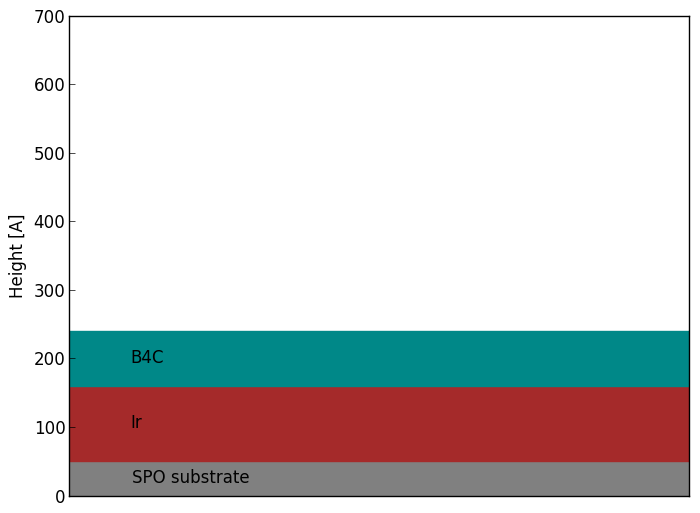
\includegraphics[width=0.4\linewidth]{figures/athena/coating_on_spo/ir-b4c-baseline.png}
  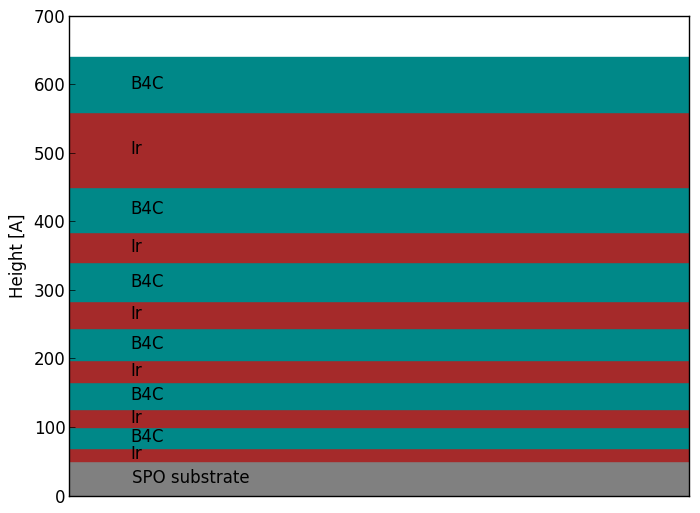
\includegraphics[width=0.4\linewidth]{figures/athena/coating_on_spo/ir-b4c-ml.png}
\caption{\footnotesize Side-view diagrams of Ir/B$_4$C coatings for Athena. \textbf{Left:} The baseline Ir/B$_4$C single bilayer. d$_{\text{Ir}} = 11.0$ nm,  d$_{\text{B}_4\text{C}} = 8.0$ nm. \textbf{Right:} The multilayer coating optimised for the middle part of the Athena optic. Consists of five bilayers with d$_{\text{min}} = 5.0$ nm, d$_{\text{max}} = 11.0$ nm, plus a cap layer of Ir of d$_{\text{Ir}} = 11.0$ nm and a top layer of B$_4$C of d$_{\text{B}_4\text{C}} = 8.0$ nm. }\label{fig:ml_baseline_sideview}
\end{figure}

The SPO substrates were coated with an Ir cathode power of 450 W and a B$_4$C cathode power of 900 W at a pressure of 2.9 mTorr with an Ar flow of 88 sccm. The base pressure was $< 2\cdot10^{-6}$ Torr.

The SPO substrates are mounted on sample plates in the chamber with ribs horizontally; the horizontal movement of the sample ensures good uniformity in the rib direction. XRR measurements performed after coating are done in the same direction along the ribs, so the coating is uniform in the footprint of the X-ray beam. In figure \ref{fig:ir-b4c-fit} can be seen an XRR measurement and IMD fit of a Ir/B$_4$C coated SPO substrate.

\begin{figure}[h!]
\centering
\begin{minipage}{.47\textwidth}
  \centering
  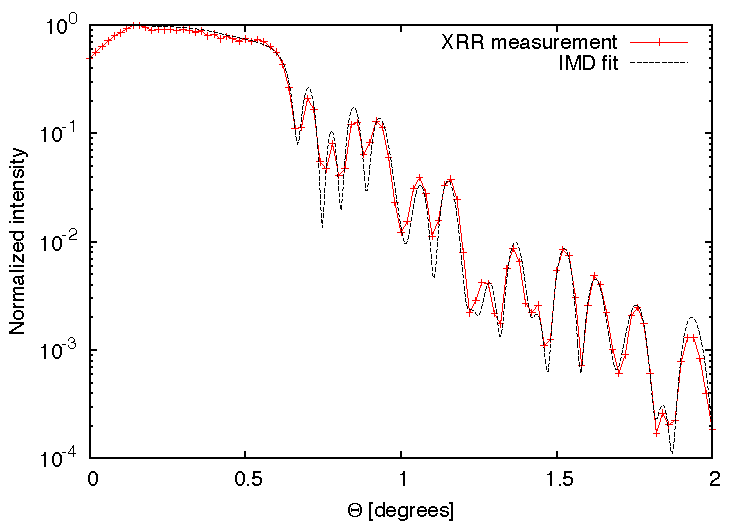
\includegraphics[width=\linewidth]{figures/athena/coating_on_spo/120-10-21_fit.pdf}
\end{minipage}%
\begin{minipage}{.53\textwidth}
  \centering
  \footnotesize
\begin{tabular}{c|c|c|c|c}
i&d$_{\text{aim}}$ [nm]&$\Gamma_{\text{aim}}$&d$_{\text{fit}}$ [nm]&$\Gamma_{\text{fit}}$\\
\hline
top&8.0&1&7.17&1\\
cap&11.0&0&11.09&0\\
1&11.0&0.6&11.43&0.620\\
2&9.5&0.6&9.99&0.617\\
3&8.0&0.6&8.54&0.623\\
4&6.5&0.6&6.95&0.576\\
5&5.0&0.6&5.85&0.567
\end{tabular}
\end{minipage}
\caption{\footnotesize XRR measurement of SPO substrate coated with optimised Ir/B$_4$C multilayer, compared to IMD model fit. Fitted values are shown to the right.}\label{fig:ir-b4c-fit}
\end{figure}

The IMD fit was done using the differential evolution algorithm\cite{Bjoerck:2011fy} included in IMD from version 5.0. The fitting results show that each layer is thicker by up to $\sim$17\% (for the thinnest layer). $\Gamma$-values are also off by $\sim$-5.5\% for the thinnest layer and $\sim$3.3\% for the thickest layer. It should be noted that the fit is not perfect and the maxima and minima of the model at lower angles that does not correspond to the data can be caused by the low-Z material not having the correct thickness.

The coated SPO substrates were also measured at the FCM beamline at the BESSY II synchrotron at PTB in Berlin. Energy scans at 1.8--10 keV can be performed there that will give an indication of the coating performance at low energies, although not at 0.1--1.8 keV. A measurement of an SPO substrate with Ir/B$_4$C multilayer coating can be seen in figure \ref{fig:spo_bessy}. Two measurements are performed at different spots to investigate non-uniformity. The reflectivity response at low energies is well-behaving, showing no sudden drops that would indicate contamination with other elements in the coating. There are two small dips at $\sim$2.1 keV and $\sim$2.5 keV, corresponding to Ir M$_{\alpha}$-edges.

\begin{figure}[!h]
  \center
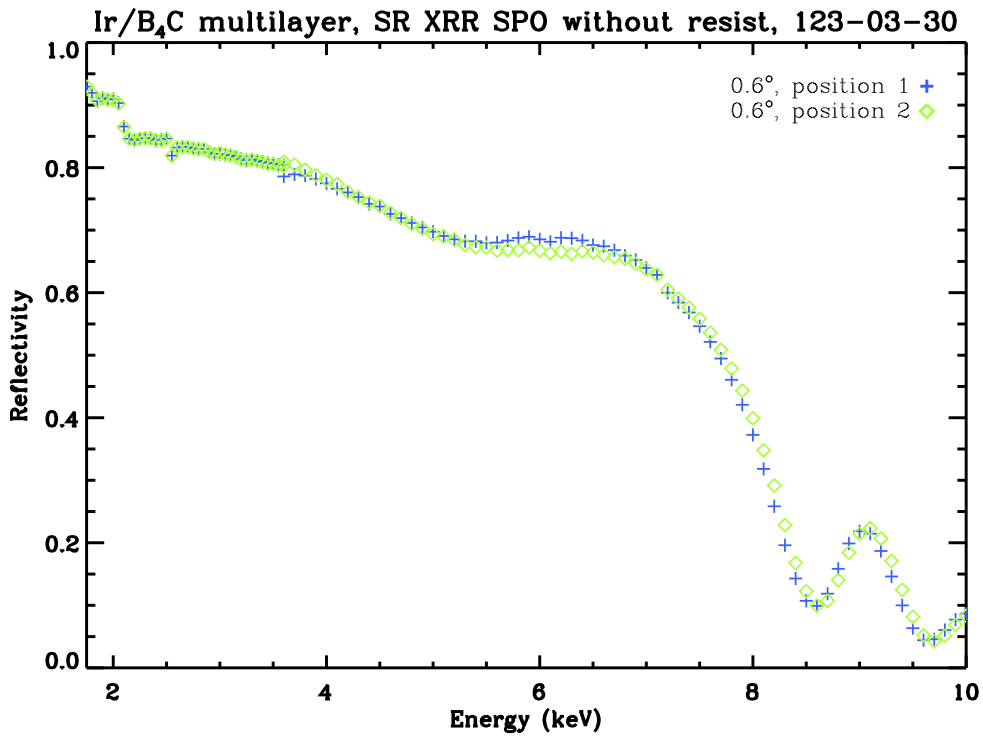
\includegraphics[height=8cm]{figures/athena/coating_on_spo/ml_irb4c_nores.jpg}
\caption{\footnotesize XRR measurements at the 1.8--10 keV energy range and a 0.6\degr\ angle, performed at the FCM beamline at BESSY II. Two measurements of the same sample are shown from different positions to investigate non-uniformity of the coating.}\label{fig:spo_bessy}
\end{figure}

\subsection{ISO qualification of Ir/B$_4$C coatings}\label{sec:qa_test}
In order to qualify the Ir/B$_4$C coatings on SPO substrates for the Athena mission, a range of tests were conducted on coated substrates. Qualification testing is a cornerstone of developing hardware for space based applications, so a number of standardisations have been developed over the years. Each standardisation applies to a specific type of hardware that needs to be qualified. The European Space Agency works with the \emph{International Organization for Standardization} (ISO) for optical devices and optical coatings. The specific tests that ESA outlines as required to qualify coated optical devices are:

\begin{itemize}
 \item A thermal cycling test according to \emph{ECSS-E-10-03A (AD4) Space engineering, testing}.\begin{quote}{\bf General purpose:} [...] of the thermal cycling test is to demonstrate the ability of the equipment under test to fulfil all functional and performance requirements over the qualification temperature range at ambient pressure.\end{quote}

 \item A humidity test according to \emph{ISO9022-2 (AD6) Optics and optical instruments, Environmental test methods, Part 2: Cold, heat and humidity}.\begin{quote}{\bf General purpose:} [...] to investigate to what extent the optical, thermal, mechanical, chemical and electrical performance characteristics of the specimen are affected by temperature and/or humidity.\end{quote}

 \item An adhesion test according to \emph{ISO9211-4 (AD5) Optics and optical instruments, Optical coatings, Part 4: Specific test methods}.
 \begin{quote}{\bf General purpose:} [...] of these tests is to evaluate to what extent the mechanical properties of optical coatings on components and substrates are affected when subjected to specific tensile or shear stress conditions at ambient atmospheric conditions.\end{quote}
\end{itemize}

Each test is described in detail in each of the documents listed above as well as the requirements that has to be met for a device or sample to succeed the test and qualify. The coated samples used in these tests were measured using XRR before and after coating as well as a visual test of the coating to quantify any changes in the coating.

Four SPO substrates were coated for qualification testing, two with single bilayer baseline Ir/B$_4$C and two with optimised Ir/B$_4$C multilayer. A baseline and multilayer sample were used for both thermal cycling and humidity tests. The samples from the humidity tests were reused for the adhesion test. All tests were carried out by David Girou from DTU Space.

The thermal cycling test consists of eight cycles in a oven (no vacuum). One cycle is divided into two hours spent at $T_{max}=85$\degr C $\pm 10$\degr C and two hours spent at $T_{min}=-45$\degr C $\pm 10$\degr C. The test is divided into two times four cycles since reflectance measurements are performed after the fourth cycle. Inital and final temperature is 22\degr C, that $\dfrac{\text{d}T}{\text{d}t}=4$\degr C$\cdot$min$^{-1}$ and that after the last cycle the temperature is first increased to 40\degr C and then decreased to 22\degr C to avoid condensation. Reflectance measurements are done after the fourth and the eighth cycle.

\begin{figure}[!h]
  \center
  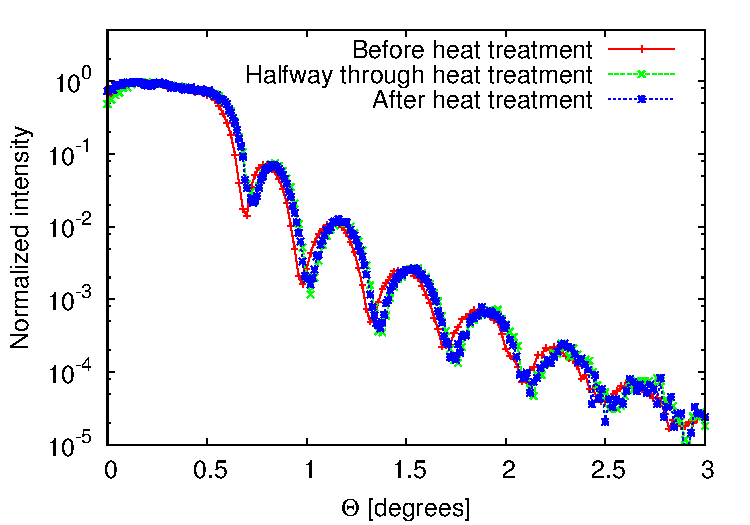
\includegraphics[width=0.47\linewidth]{figures/athena/coating_on_spo/123-10-12_cooked_2.pdf}
  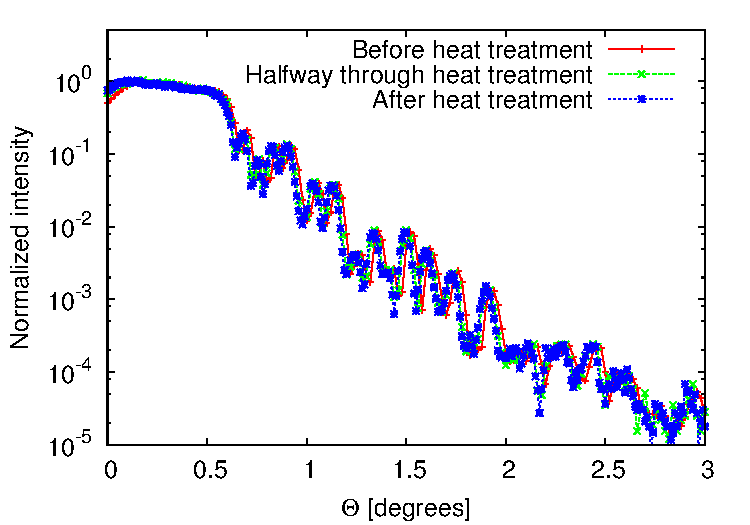
\includegraphics[width=0.47\linewidth]{figures/athena/coating_on_spo/120-10-21_cooked_2.pdf}
\caption{\footnotesize XRR measurements of Ir/B$_4$C coatings on SPO substrates before thermal cycling test, after four cycles, and after eight cycles. \textbf{Left:} Baseline Ir/B$_4$C coating. \textbf{Right:} Multilayer Ir/B$_4$C coating.}\label{fig:qa_temp}
\end{figure}

Results of the temperature test can be seen in figure \ref{fig:qa_temp}. No change is apparent apart from a misalignment of the first XRR measurement by 0.02\degr\ of both the baseline and multilayer (red lines).

The humidity test consists of 48 hours spent at a temperature of 40\degr C and a relative humidity between 90\% and 95\%. Samples are measured with XRR before and after the humidity test, results can be seen in figure \ref{fig:qa_hum}. No change in the baseline or multilayer XRR measurements after the humidity test.

\begin{figure}[!h]
  \center  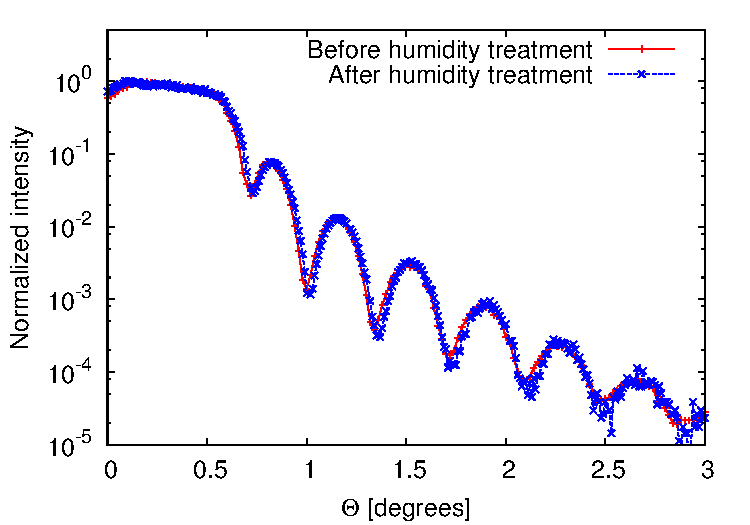
\includegraphics[width=0.47\linewidth]{figures/athena/coating_on_spo/123-11-09_hum_2.pdf}
  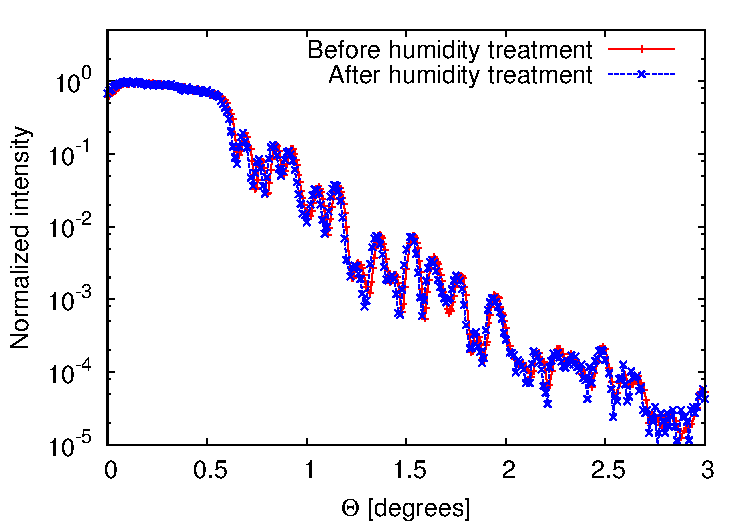
\includegraphics[width=0.47\linewidth]{figures/athena/coating_on_spo/120-09-26_hum_2.pdf}
\caption{\footnotesize XRR measurements of Ir/B$_4$C coatings on SPO substrates before and after a humidity test. \textbf{Left:} Baseline Ir/B$_4$C coating. \textbf{Right:} Multilayer Ir/B$_4$C coating.}\label{fig:qa_hum}
\end{figure}

The adhesion test was performed using a 25x19 mm$^2$ piece of scotch tape applied firmly to the surface of the coating on the SPO substrate. The tape was subsequently snapped rapidly off the surface. A visual inspection of the surface is performed afterwards. The degree of success of the test is measured in how rapidly the tape is pulled off without taking the reflective coating with it. No amount of pulling could remove neither the baseline nor multilayer Ir/B$_4$C coating. XRR measurements were also done on the samples to ensure that the top B$_4$C was not removed. As can be seen in figure \ref{fig:qa_adh}, both multilayer and baseline coating were unharmed in the test.

It is worth noting that the Ir/B$_4$C coatings applied to the SPO substrates were without a Cr underlayer to decrease the film stress. With that in mind, the Ir/B$_4$C baseline and multilayer can be expected to have had film stress of $\sim-$4 GPa and $\sim-$2 Gpa respectively[\ref{pap:PREL_Athena}].

\begin{figure}[!h]
  \center  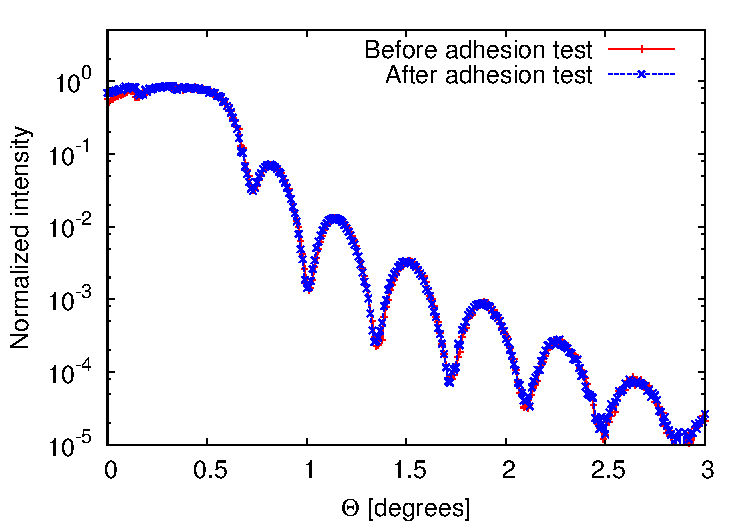
\includegraphics[width=0.47\linewidth]{figures/athena/coating_on_spo/123-11-09_adh_2.pdf}
  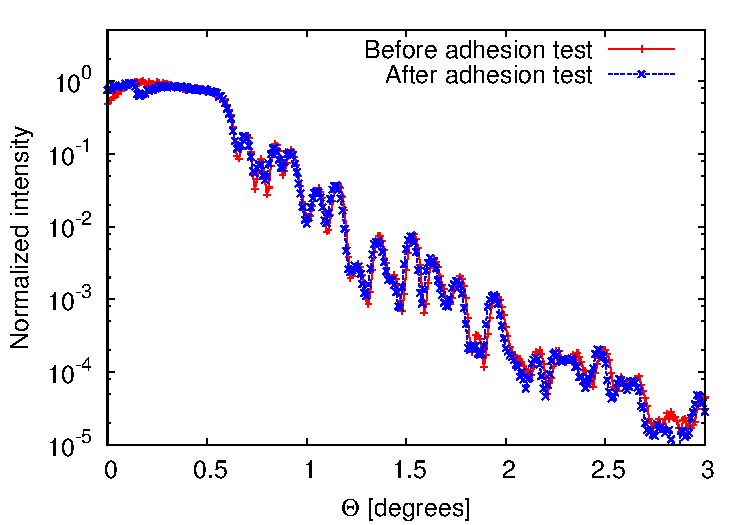
\includegraphics[width=0.47\linewidth]{figures/athena/coating_on_spo/120-09-26_adh_2.pdf}
\caption{\footnotesize XRR measurements of Ir/B$_4$C coatings on SPO substrates before and after an adhesion test. \textbf{Left:} Baseline Ir/B$_4$C coating. \textbf{Right:} Multilayer Ir/B$_4$C coating.}\label{fig:qa_adh}
\end{figure}


\section{Upscaled production}\label{sec:Athena_upscaled}

%\emph{The following section was part of a technical report for the European Space Agency. It was done as part of the coating investigations for the original Athena proposed for ESA's L1 mission, which had a double-telescope configuration. It also required significantly less silicon pore optic substrates, 64,640 vs. $\sim$130,000 for Athena. The investigations done for scaling up production still holds true and the final production will also still take 2 years, but cost, production equipment and manpower will have to increase by a factor of two to three.}

For the Athena mission, the coating of the mirror substrates will be a large undertaking as 140,030 silicon pore optic (SPO) substrates will need a coating of between two and twenty layers.

Every piece will have to be transported from the SPO substrate fabrication facility (SFF) to a new dedicated coating facility, thoroughly cleaned, coated in specially designed chambers and then transported to the stacking facility. After stacking into mirror modules (MM), each MM will be measured at one of three dedicated beam lines at the BESSY II synchrotron in Berlin.

In this paper, an estimate of cost and timeframe of the coating and coating qualification of all SPO substrates for the Athena mission is given.

\subsection{Timeline and cost of procurement and setup of coating facility}

Cleaning and coating of SPO substrates will require as a minimum an ISO 7 clean room to avoid dust particles. Dust on the substrates before coating will result in small holes in the coating, which will reduce the effective area. There are two possibilities for the location of the coating facility which is discussed in this paper. Either the facility is located in the same building or adjacent building as the stacking facility or the coating facility is placed further away, i.e. another country within Europe.

Moving substrates in and out of clean rooms and transporting them over larger distances has drawbacks and extra costs associated. But locating the two facilities separately can reduce costs as it will be easier cheaper to find two smaller clean rooms to re-purpose into production facilities. Building and setting up clean rooms of a sufficient size for both facilities will take several years and come with a significant cost, but if it is possible to re-purpose existing laboratories that cost can be reduced.

The first part of the clean room should be for opening shipments from the SFF and cleaning each substrate. As the substrates are produced in a clean room at the SFF, it is assumed that they will at maximum need to be cleaned with an air gun with dry nitrogen. After being cleaned, each substrate is mounted onto a substrate holder that will be inserted into a coating chamber for coating. When the coating is done, the substrate holder is taken out of the chamber and the substrates are ready to go into the stacking facility.

Clean rooms can be build inside existing larger storage areas or cleaner production facilities. The approximate timeline for the setup of the entire facility is as follows:

\begin{description}[itemsep=1.5pt,parsep=1pt]
	\item[9] \textbf{years before launch:}
		\begin{itemize}[itemsep=1.5pt,parsep=1pt]
		\item[-] Planning begins for the construction of a shared cleanroom facility.
		\item[-] Planning begins for coating chambers.
		\end{itemize}
	\item[7-8] \textbf{years before launch:}
		\begin{itemize}[itemsep=1.5pt,parsep=1pt]
		\item[-] Construction of facility is carried out.
		\item[-] Produced coating chambers are installed and qualifications begun.
		\end{itemize}
	\item[6] \textbf{years before launch (CDR):}
		\begin{itemize}[itemsep=1.5pt,parsep=1pt]
		\item[-] Coating capabilities ready.
		\end{itemize}
\end{description}

The cost of building and preparing the coating facility will differ between a shared facility and separated facilities, but the coating chambers will have a similar configuration.

\subsection{Coating chambers}\label{sec:chambers}
The telescope of Athena consists of 19 rings of mirror modules, each with two stacks of 68 coated SPO substrates, resulting in 140,030 SPO substrates in total. Considering the coating chamber design used at DTU Space, a maximum of 100 plates can be coated per day in an 8 hour workday. In a year of 200 workdays, 20,000 substrates can be coated. Using six chambers, 120,000 substrates can be coated per year, within the two year time frame a total of 240,000 substrates can be coated. A minimum of 1.5 times the needed 140,000 coated substrates is considered the baseline ($\sim$210,000), as we account for damaged plates, bad coatings etc. That leaves an acceptable down time of $\sim$2 months throughout the project.

Using chambers of same design as DTU Space will give a cost of around 1M \euro\ per chamber. Those chambers have the drawback of a long pump down time after having the chamber opened to change samples. The advantage of coating SPO substrates compared to e.g. NuSTAR glass is that the SPO substrates are flat and only $\sim$1 mm thin.

If a new chamber design is considered, it would be advantageous to pursue a design similar to what is used in the semiconductor industry. Here an entire wafer are given a number of different coatings and automatically moved from one cathode to another using a robotic arm. As those wafers can have a thickness of up to 3 mm, we propose to use a substrate holder shaped like a wafer 3 mm thick with a diameter of 300 mm. Recessions in the substrate holder can accommodate SPO substrate and no clips will be needed to hold substrates in place, since the wafer will at all times be horizontal. A chamber of that design will not need pump down time between each batch of substrates, since wafers will be inserted into the central vacuum chamber through a narrow slit directly from a clean magazine in atmospheric pressure. Every coating cathode is also in a separate chamber and can be accessed without venting the entire machine. Custom made machines like seen in figure \ref{fig:dram} are priced at $\sim$2M \euro.

\begin{figure}[htbp]
	\centering
		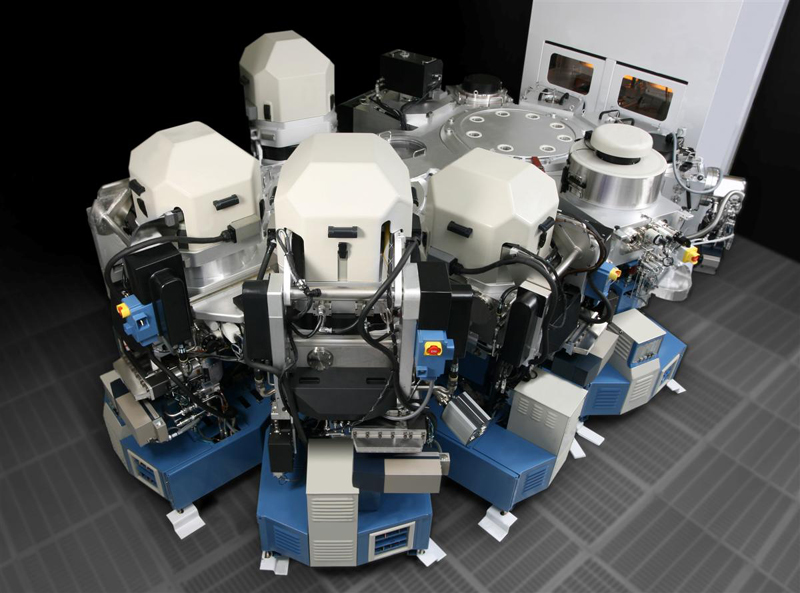
\includegraphics[width=0.7\textwidth]{figures/athena/dram.jpeg}
	\caption{\footnotesize Multi-chamber deposition machine from Applied Materials. Each white dome is a sputtering chamber with a circular cathode depositing downwards. Wafers are moved between chambers using a robotic arm  placed in the central vacuum chamber. \emph{Source: www.appliedmaterials.com}}
	\label{fig:dram}
\end{figure}

A significant increase in production rates can be achieved using machines like this. It also gives a cleaner environment for samples, since the machine itself can stay closed for longer periods of time. Higher production rates means that only three or four chambers are needed to complete the coating of 210,000 SPO substrates in two years.

\subsection{Shared facility}
Since both the coating facility and stacking facility needs a clean room, these can be combined or connected in a shared facility. If the chamber design from DTU Space is used, a separate clean room will be needed to accommodate these chambers as they can give off dust flakes of material every time they are opened. If instead a multi-chamber coating system is used as described in section \ref{sec:chambers}, the coating machinery can be in a separate clean room against the wall into the stacking facility. That way wafer cassettes full of wafer-shaped SPO substrate holders can be inserted and retrieved from the stacking facility clean room.

For a shared facility with multi-chamber coating systems as described in section \ref{sec:chambers}, we propose the following facility setup:

\begin{itemize}
	\item Common class 10,000 clean room for mounting SPO substrates on wafer-shaped sample holders. The same room will be used for fast X-ray system for pre- and post coating measurements.
	\item Access to insertion port of multi-chamber coating system from the common clean room. Wafer cassettes are mounted directly to accessible part of the machine.
	\item The back end of the coating chambers are in a separate room, so targets can be changed without giving off dust near the substrates.
	\item In connection to the common clean room is a separate class 100 - 10,000 clean room with stacking robots. The robots can be in a separate ventilated tent inside the clean room to decrease particle dust. Mirror modules will be sealed here and moved outside the clean rooms for packing and shipping to BESSY II.
\end{itemize}

\subsection{Separated facilites}
If the facilities are separated, a large effort will be required to keep substrates clean when packing/unpacking for transport. The substrates will be send from the SFF in batches of 3,000 and double or triple sealed, so the package can be opened partly when inside a moderately clean room and opened completely in the main class 10,000 clean room. The following setup of clean rooms is proposed.

\begin{itemize}
	\item Two separate class 10,000 clean rooms, one for substrate handling and one for coating chambers. Alternatively, one larger clean room parted by a clear plastic curtain.
	\item Substrate handling clean room will also be used for the fast X-ray system for pre- and post coating measurements.
	\item Coated samples will be packed and double sealed inside the clean room before being shipped to the stacking facility.
\end{itemize}

\subsection{Resist deposition and removal at alternative facility}
One of the processes done at the SFF to the substrates before sending them to the coating facility will be the lithographic process of resist deposition. It requires a semiconductor grade facility to apply the resist using spray-on and afterwards removing stripes by a UV radiation process.

The process can, instead of at the SFF, be done either at the coating facility by including the proper equipment or at an external facility. DTU Danchip is the Danish National Center for Micro- Nanofabrication, which runs a class 10 clean room with equipment capable of depositing the resist and UV curing the SPO substrates.

The removal of the resist after coating can be done at the stacking facility, but can also be done at the coating facility if these are separated. By doing the resist removal at the coating facility, a visual inspection can be done of the substrate before being transported to the stacking facility. If the process damages the coating, the problem can be located and new coated substrates can be produced quickly.


\subsection{Cost for setting up}
To prepare the lab before the coating campaign starts, the coating chambers will need to be installed and configured. An extensive campaign with scientific personnel is needed to ensure the system's capability to produce coatings of sufficient quality. We estimate 12-24 months to qualify the coating chambers for the Athena coating campaign and will need approximately four scientific personnel and two technicians.

The coating qualification equipment described in section \ref{qualification} will be needed to qualify the coating chambers.


\begin{table}[htbp]
	\centering
\begin{tabular}{l|c}
Equipment & Approx. price \\
\hline
\hline
6 x Coating chambers of DTU design  & 6 x 1,000,000 \euro\\
\hline
or:\\
\hline
4 x Multi-chamber coating systems & 4 x 2,000,000 \euro \\
\hline
\\
\hline
Personnel for setup & 980,000 \euro\\
\end{tabular}
\end{table}


\subsection{Timeline and cost for production of Athena coatings}
SPO substrates are fabricated at the SFF and should be shipped to the coating facility weekly in shipments of 3,000 substrates. 600 substrates are daily mounted on wafer shaped sample holders after they have been measured using the fast X-ray system. The substrates are coated in one of the coating chambers and subsequently taken out to have resist removed and be measured again using the fast X-ray system.

Cost drivers during production are sputtering targets and personnel. The final cost is dependent on which material combination is used for coating. The differences can be seen below.

\begin{table}[htbp]
	\centering
\begin{tabular}{l|c|c|c|c}
Material 	& High Z 		& Approximate & Low Z  & Approximate \\
combination & thickness & price / mm$^3$ & thickness &  price / mm$^3$ \\
 & (nm) & (High Z) & (nm) &  (Low Z) \\
\hline
\hline
Cr/Ir/B$_4$C & 10 & 10.9 \euro & 8 & 0.26 \euro\\
\hline
Pt/B$_4$C & $\sim$16 & 10.5 \euro & $\sim$22 & 0.26 \euro\\
\hline
W/B$_4$C & $\sim$16 & 0.73 \euro & $\sim$22 & 0.26 \euro\\
\end{tabular}
\end{table}

The approximate cost is calculated based on a 10\% efficiency of the sputtering cathodes, meaning 10\% of the target material ends on a substrate. For a single layer of 10 nm on all the substrates of Athena, the volume of material needed will be approximately 10 cm$^3 = $ 10,000 mm$^3$. From that, the total target cost can be estimated.

\begin{table}[htbp]
	\centering
\begin{tabular}{l|l|c|c}
Material 	& Type of coating & Approx. cost & Approx cost incl. \\
combination	&	&	&	30 \% target \\
&	&	&	usability\\
\hline
\hline
Cr/Ir/B$_4$C & Tri-layer & 114,000 \euro & 380,000 \euro \\
\hline
Pt/B$_4$C & Graded-d multilayer & 174,000 \euro & 580,000 \euro\\
\hline
W/B$_4$C & Graded-d multilayer & 17,400 \euro & 58,000 \euro \\
\end{tabular}
\end{table}

Only 30\% of the target can be used before it has to be replaced, so a factor of 3-4 should be applied to these cost estimates. The leftover targets of precious metals, platinum and iridium, can be sold back at market value, which can reduce the total costs of precious metal consumption by up to $\sim$50 \%.

For a Pt/B$_4$C graded-d multilayer, the total thickness of Pt is 16 nm in average and 22 nm of B$_4$C. Thus, $1.6 \cdot 10000$ mm$^3$ of Pt is needed at a price of 10.5 \euro\ per mm$^3$ at 90 \% coating loss, combined with $2.2 \cdot 10000$ mm$^3$ of B$_4$C at 0.26 \euro\ per mm$^3$ gives a total cost of 174,000 \euro.

\subsection{Personnel}
During the two year coating campaign, 600 substrates will be handled daily. Procedures to be done daily include:

\begin{itemize}[itemsep=1.5pt,parsep=1pt]
	\item Unpacking substrates.
	\item Measuring using fast X-ray system.
	\item Mounting substrates on sample holders.
	\item Load sample holders in coating chamber.
	\item Running coating equipment.
	\item Unloading sample holders.
	\item Remeasuring using fast X-ray system
	\item Repacking samples for transport to stacking facility.
\end{itemize}

Additionally, the coating chambers will require new targets to be installed on a weekly basis. We estimate 4-5 technicians are needed in addition to 3-4 scientific personnel to run the coating production.

For five technicians four scientists, a two year coating campaign will cost $\sim$2,800,000 \euro.

%\subsection{Shared facility}
%\subsection{Separated facilites}

\subsection{Coating QA during production}\label{qualification}
We envision a significant coating qualification campaign for the Athena mission. We propose a fast automated 8 keV X-ray setup, that can measure every plate before and after coating. The plan is to make reflectivity scan of ca 50 \% of the pores.  Each measurement is an angular scan  at a fixed 8 keV energy and at an angular range of 0\degr to $\sim$ 1.5\degr\ will determine micro roughness to an accuracy of +/- 0.02 nm. It till require automatic alignment to an accuracy of +/- 0.01\degr. Measurements for each plate should be conducted in less than 5 minutes and each scan should be automatically fitted, with the data logging and plotting part of the facility. The foot print of the beam should cover more than 10 \% of each pore.

The total database of reflectivity measurements can be used when building the final optical response model for Athena. During the campaign it will be required to measure ~1,200 SPO substrates per day, so the system should be capable of measuring each substrate in a batch automatically.

Every chamber needs to be calibrated twice a week to ensure a precise layer thickness. This will require samples to be coated with constant-d multilayers, which will be measured using a separate 8 keV X-ray reflectivity (XRR) setup at the facility.

In every coating run, a witness sample will be included along with SPO substrates. These witness samples will be measured using the 8 keV XRR setup to ensure proper layer thickness interfacial roughness. In addition, 5x70 mm wafer pieces are also coated measured for stress using a stylus measurement tool. One or two times a week, a coated SPO substrate will be taken out to check for adhesion and visual QA in a microscope. If contamination is suspected, an AFM analysis will be carried out, if necessary externally.

Measuring samples at the energies visible by Athena can help build the final optics model. We propose this optional addition: A single coated substrate per day will be selected for reflectivity scatter measurements at the BESSY II synchrotron at PTB Berlin. 25 substrates per month can be measured using X-ray reflectivity energy scans at 4 to 10 keV at BESSY II within 2-3 days. A few more days per month will be needed to measure scattering from select substrates.

Below are approximate prices for equipment needed.

\begin{table}[htbp]
	\centering
\begin{tabular}{l|c}
Equipment & Approx. price\\
\hline
\hline
Fast automated 8 keV X-ray setup  & 1,000,000 \euro\\
\hline
Separate 8 keV X-ray setup & 500,000 \euro\\
\hline
Stylus stress measurement setup & 30,000 \euro\\
\end{tabular}
\end{table}



\subsection{Timetable and cost}

The timetable is independent on whether the coating facility is shared with the stacking facility or separate.\\

\begin{table}[htbp]
	\centering
\begin{tabular}{c|l}
T - 9 years & Planning begins for the construction\\
  & \hspace{1cm} of a shared clean room. \\
			& Planning begins for coating chambers.\\
\hline
T - 8 years & Construction of facility is carried out.\\
			& Produced coating chambers are installed\\
      & \hspace{1cm} and qualifications begin.\\
\hline
T - 7 years & Continuation of coating chamber qualifications.\\
\hline
T - 6 years & Coating chamber qualifications complete.\\
			& Coating capabilities ready.\\

\end{tabular}
\end{table}

The timetable gives the possibility of starting the coating campaign six years before launch. The coating campaign is set for two years including delays will have the optic ready four years before launch. The four year window between optic readiness and launch is specified in the ESA timetable.

Total cost for a shared facility is calculated below. For a separate facility, transport costs of substrates will have to be included, estimated at minimum 100,000 \euro. Substituting six DTU design coating chambers with four more advanced multi-chamber systems will increase the cost of coating chambers from 6 mio. \euro to 8 mio. \euro, but the possible improvement in cleanliness and uptime will in our opinion make up for the difference.

\begin{table}[htbp]
	\centering
\begin{tabular}{l|c}
Expense & Approx. price\\
\hline
\hline
6 x Coating chambers of DTU design  & 6 x 1,000,000 \euro\\
\hline
or:\\
\hline
4 x Multi-chamber coating systems & 4 x 2,000,000 \euro \\
\hline
\\
\hline
Fast automated 8 keV X-ray setup  & 1,000,000 \euro\\
\hline
Separate 8 keV X-ray setup & 500,000 \euro\\
\hline
Stylus stress measurement setup & 30,000 \euro\\
\hline
Sputtering targets & 600,000 \euro\\
\hline
Personnel during setup & 2,000,000 \euro\\
\hline
Personnel during production & 3,000,000 \euro\\
\hline
\textbf{Total} & $\leq$ 15,130,000 \euro\\
\end{tabular}
\end{table}

\section{Athena discussion and conclusion}
The Athena mission is set to launch in 2028 and it is clear that many things has to fall into place to meet the deadline, especially the large production effort that has to be realised. From the results in described in this chapter, the choice of Ir/B$_4$C material combination seems to be the only possibility to meet the target of 2 m$^2$ effective area at 1 keV. An alternative material combination that could work with the lithographic process described in section \ref{sec:Athena_opt_tech} is W/Si, but the higher electron density of Si would seriously impact the effective area at lower energies and so would the absorption edge of Si at $\sim$1.8 keV.

Selecting B$_4$C as the low-Z material in the reflective coating is an obvious choice for an X-ray telescope with sensitivity down to 0.1 keV, but as this chapter shows, there are serious problems with B$_4$C in combination with Pt or W. Reflective W/B$_4$C multilayer coatings for X-ray purposes has been reported in the litterature\cite{Jankowski:1991kx,Morawe:2007vp}, but none has shown the long term effect ambient conditions can have on these coating. Some report on the stability of W/B$_4$C multilayers after heat treatment to 500\degr C\cite{JANKOWSKI:1990vd} or 800\degr C\cite{Rao:2013dt}, but both were done under vacuum ($<10^{-4}$ Torr).

Extensive investigations in the literature has shown no reports on the deposition of a Pt/B$_4$C multilayer combination, so this chapter provides the first measurements of the coating and long term stability. The multilayers were found to have a high interlayer roughness by XRR immediately after coating, so it was decided to use a single Pt/B$_4$C bilayer as a backup solution to the Ir/B$_4$C baseline because of the lower stress. However, the long term stability tests revealed what seems to be a large amount of diffusion at the Pt/B$_4$C interface, leading to a break-down of the multilayer structure. Even in a single bilayer film the high amount of diffusion will significantly increase interlayer roughness over time.

The changes in both Pt/B$_4$C and W/B$_4$C over time seems to be only under ambient humidity, i.e. not an issue after launch; but keeping every single coated SPO substrate out of humidity for 4--6 years during production and until launch is not quite realistic. The end result is a complete disqualification of both Pt/B$_4$C and W/B$_4$C for Athena in favor of Ir/B$_4$C single bilayer or multilayers and with W/Si as a backup solution, although without meeting science requirements of 2 m$^2$ effective area at 1 keV.

The qualification tests of Ir/B$_4$C coatings on SPO substrates described in section \ref{sec:qa_test} showed great promise in the stability of the material combination even under high humidity and temperature. Later tests were done to see how high a temperature the coatings can withstand before breaking down, and at 250\degr C, a change was seen in structure in XRR measurements. The high stress of the materials that was seen early in the investigations can be mitigated using a Cr underlayer, and the high surface roughness of Cr can be mitigated by a unique smoothening effect of Ir. Even without a Cr underlayer, it seems that the high stress has no consequence on the stability of the coatings; and as the SPO substrates are extremely stiff, no bending is likely to occur as a result of film stress.

The choice between single bilayer or multilayer Ir/B$_4$C coatings for Athena is a question of cost. Applying a single bilayer is the inexpensive solution, as it puts the least requirements on production facilities; every SPO substrate will get the same coating. Multilayers of 5--10 bilayers will require more time per sample to apply as well as more complicated coating chambers. One could imagine a linear coating system with one Ir cathode and one or two B$_4$C cathodes, SPO samples would enter in one end of the system and exit in the other end, thereby finishing a baseline single bilayer coating with just a linear movement through the chamber. A similar setup for multilayer coatings would require a system with up to 20 cathodes in a row of interchanging Ir and B$_4$C, a massive system with multiple points of failure. An alternative approach is the multi-chamber solution as described in section \ref{sec:chambers}, which is the recommended solution reported to ESA by DTU Space. The multi-chamber coating facility takes advantage of the SPO technology heritage from the semi-conductor industry, primary advantage being the completely flat geometry of SPO substrates before stacking.

The past decades of rapid growth and technological progress in the semi-conductor industry will definitely be a major reason for making a telescope with more than 140,000 mirror substrates possible. A similar sized mission with individually slumped glass substrates as in the NuSTAR mission will require a substantial man-power effort as each step from flat glass to curved, cleaned and coated glass mirrors are labor-intensive and almost impossible to automate. The SPO technology has drawbacks, such as limits on material combinations and a larger minimum inner radius compared to slumped glass, but the low substrate figure error, mass production capability, and rigidity of mirror modules gives SPO a substantial advantage in large X-ray missions.

\chapter{Coatings for CAST}
After the launch of NuSTAR, the X-ray optics group at DTU Space was invited to participate in the creation of an X-ray optic for the CAST solar axion helioscope \cite{Elias:1387488,Iguaz:1389411}. CAST is an experiment at CERN that looks for the hypothetical axion particle\cite{Weinberg:1978ii,Wilczek:1978kp,Peccei:1977ea,Peccei:1977em} which is a solution to the charge-parity (CP) problem of the standard model in particle physics\cite{Cheng:1988fu}. If the axion exist, it is also some or all of the dark matter in the universe\cite{Visinelli:2011tw,Bae:2008ix}. It was decided that the optics technology from NuSTAR\cite{Christensen:2011wg,Harrison:2010gu,Koglin:2005kb,Zhang:2009cb,Harrison:2013wl} could be leveraged and therefore use spare glass to make a cheap and relatively simple X-ray optic.

The optic was designed between summer 2012 and summer 2014. Production, assembly, installation and alignment with CAST was done during summer 2014 in cooperation with University of Zaragoza (UoZ) in Spain and Lawrence Livermore National Lab (LLNL) in the US. In this chapter the reader will find a description of the whole process from start to finish.

My part of the work was to design the optic geometry and coating as well as produce the coated substrates and participate in the installation. LLNL designed vacuum vessel and alignment procedure and UoZ designed detector and X-ray source assembly.

A complete software package was developed that could calculate the geometry of the optic given a focal length and substrate specifications. The software then optimises the coating for a range of material combinations with respect to energy range and axion spectrum by incorporating IMD. I chose to make the software in Python because of the huge amount of documentation and specialised packages available. To interface with IMD, a package called Pidly was used to communicate with IDL, which could spawn an IMD session. The principle is described in section \ref{sec:software_improvements}

\section{The CAST instrument}
The axion is an ultra-light particle that is formed from the interaction of a photon with an electromagnetic field, called the Primakoff effect. So the main sources of the particle would be from inside stars, and from Earth the best nearby source will of course be the Sun. The axion is weakly interacting so in order to detect it, CAST uses a strong magnet to convert the axion back to a photon, again by the Primakoff effect. The photons subsequently hit a detector.

\begin{figure}[htbp]
  \centering
    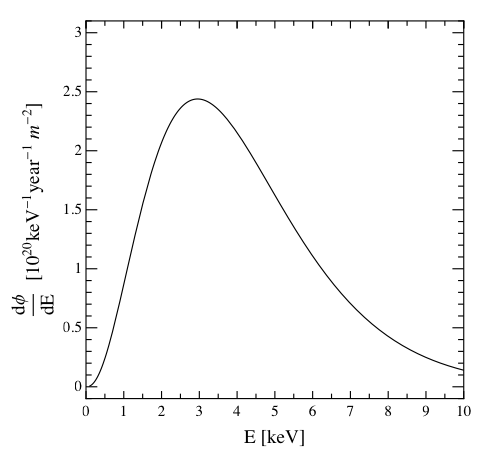
\includegraphics[height=6cm]{figures/cast/axion_spectrum.png}
  \caption{\footnotesize Solar axion flux spectrum at Earth. }
  \label{fig:axion_spectrum}
\end{figure}

The spectrum of X-rays from solar axions reaching Earth can be seen in figure \ref{fig:axion_spectrum}. It is relatively low energy X-rays with a peak around 3 keV and a shape similar to the black-body radiation spectrum.

\begin{figure}[htbp]
  \centering
    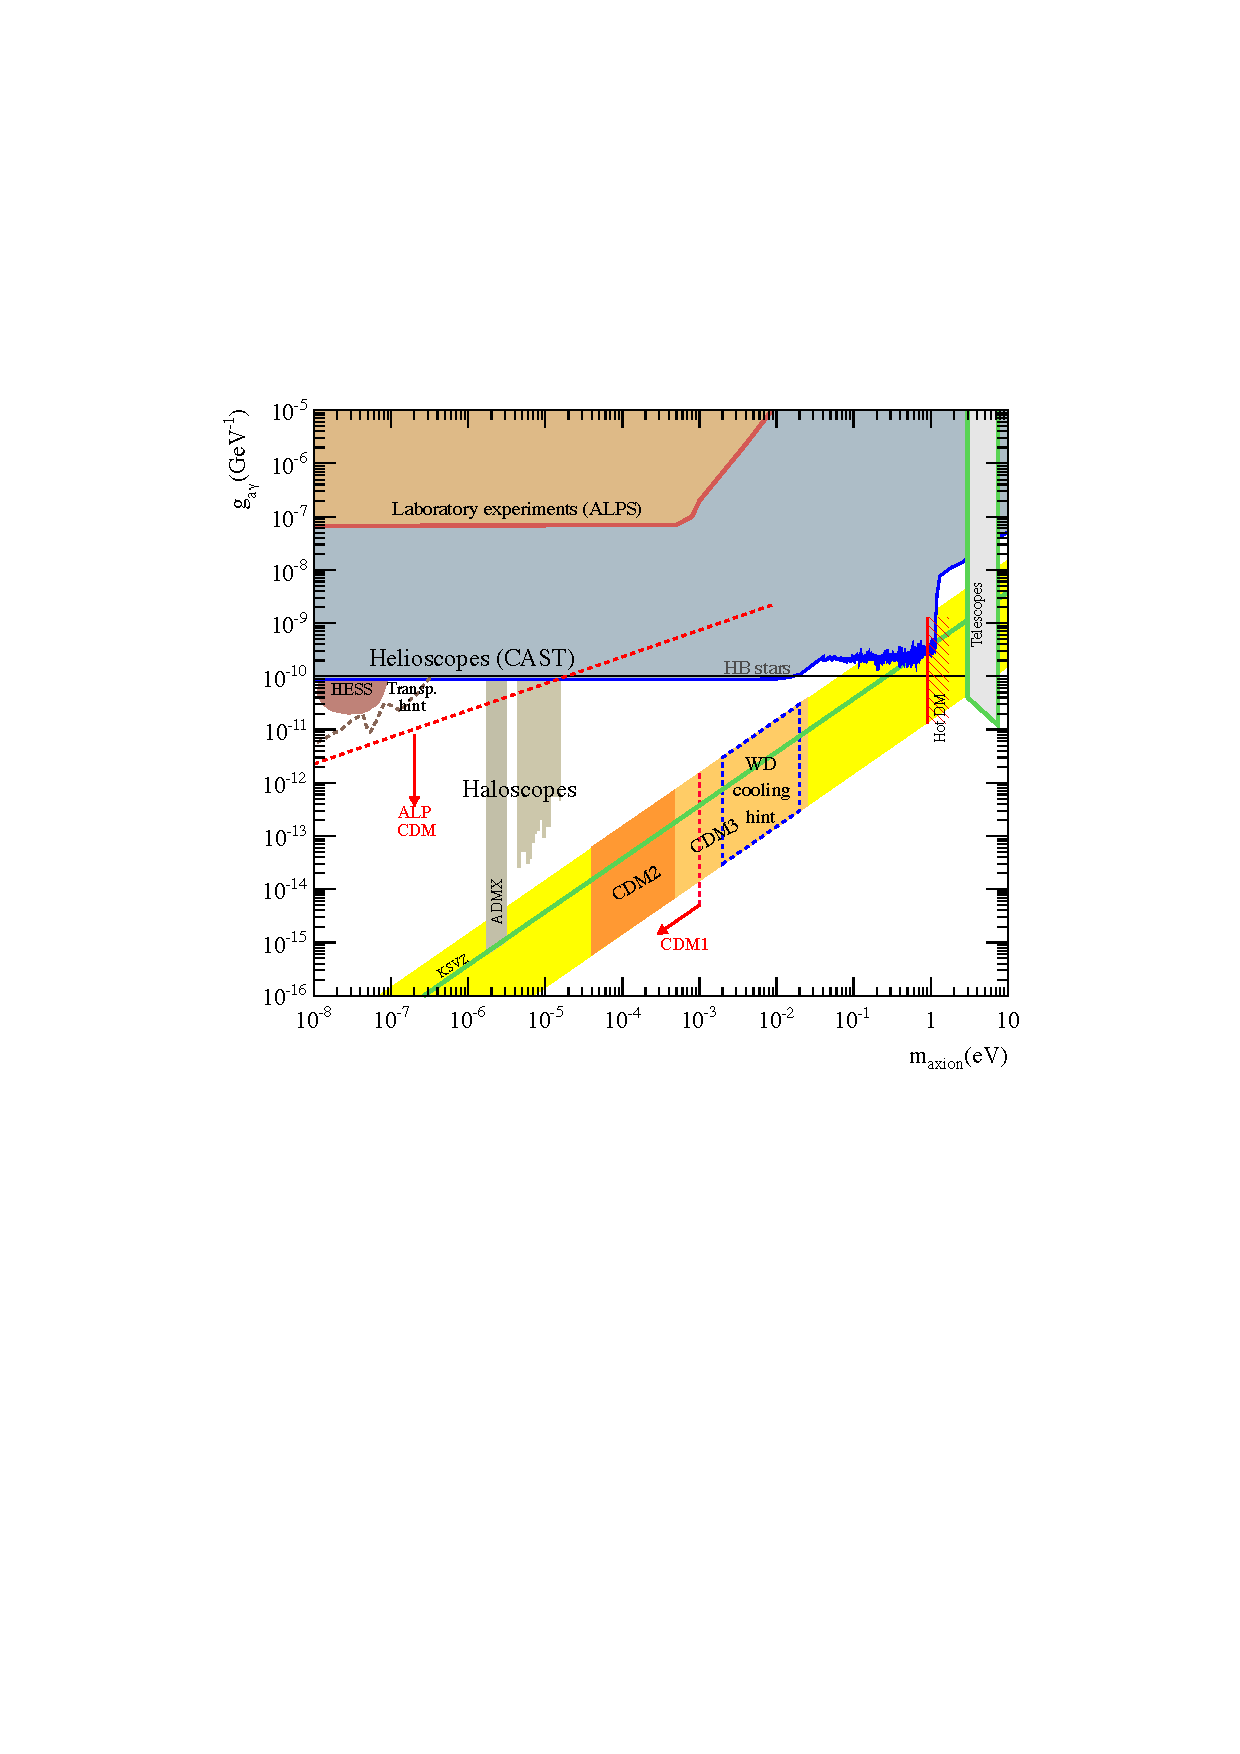
\includegraphics[height=6cm]{figures/cast/axion_search_cast2.pdf}
  \caption{\footnotesize The axion (and axion-like partikle) parameter space, showing the limits of detection for current direct detection experiments. The yellow "axino band" represents areas of the parameter space where theoretical models predicts axions. The part of the parameter space excluded by the CAST axion helioscope so far is represented by the blue line and grey area. (From \cite{Irastorza:2013uu})}
  \label{fig:axion_search_cast}
\end{figure}

From theory, the expected mass of the axion is between $10^{-7}$-$1$ eV. In figure \ref{fig:axion_search_cast} the parameter space can be seen with the axion-photon coupling constant, \gay, as a function of the axion mass, \maxion. The yellow line represents the area where we expect to see the axion if all dark matter in the universe consists of axion particles with the same \maxion\ and \gay. The CAST helioscope is by 2014 the most comprehensive axion search, and has set an experimental upper limit of
\begin{eqnarray}
\gaymath \leq 8.8 \cdot 10^{-11} \textrm{ GeV}^{-1}\cite{Zioutas:2005jl,Andriamonje:2007jc}.
\end{eqnarray}
% \begin{figure}
% \centering
% \begin{minipage}{.5\textwidth}
%   \centering
%   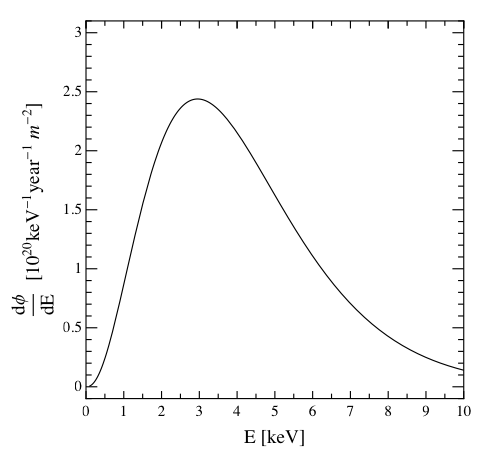
\includegraphics[height=4.6cm]{figures/cast/axion_spectrum.png}
%   \captionof{figure}{A figure}
%   \label{fig:axion_spectrum}
% \end{minipage}%
% \begin{minipage}{.5\textwidth}
%   \centering  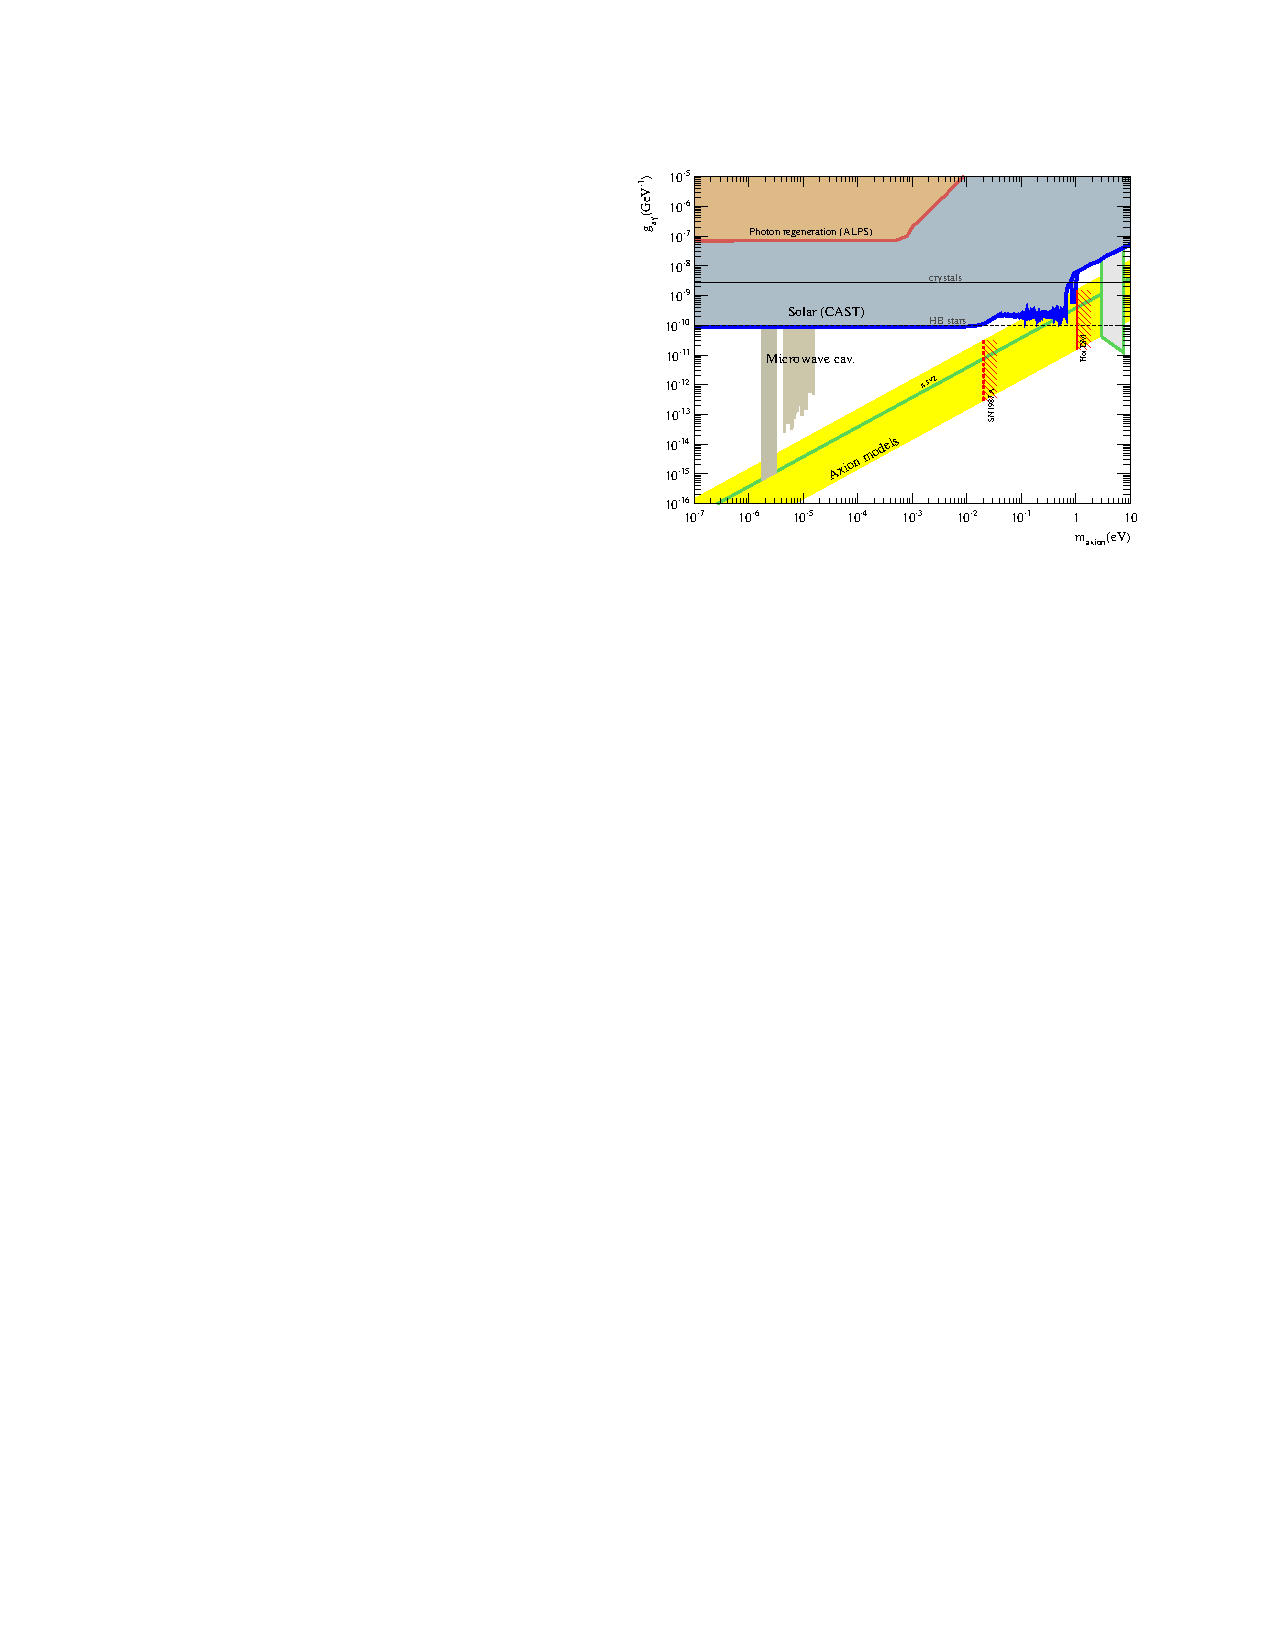
\includegraphics[width=\linewidth]{figures/cast/axion_search_cast.pdf}
%   \captionof{figure}{Another figure}
%   \label{fig:axion_search_cast}
% \end{minipage}
% \end{figure}
The CAST experiment is largely made from spare parts of other projects at CERN and other research institutions. The magnet is one of three prototype superconducting dipole magnets from the Large Hadron Collider. It is designed to transport particles in two directions inside a strong magnetic field, so it has two bores inside with diameters of 43 mm. As can be seen in the picture of the CAST instrument (figure \ref{fig:cast_instrument}), the magnet is able to pitch and yaw up to a limit. That makes it possible to follow the sun as it comes up with one end, and as it goes down with the other end. Since the axion does not interact with matter, detectors are placed at both ends of the magnet and at both boreholes, so two detectors can be used at sunrise and two at sunset. The detectors used are low-background time projection chambers with MicroMegas readouts \cite{Giomataris:1996eo,Giomataris:2006fy,Andriamonje:2010jh}.

\begin{figure}[htbp]
  \centering
    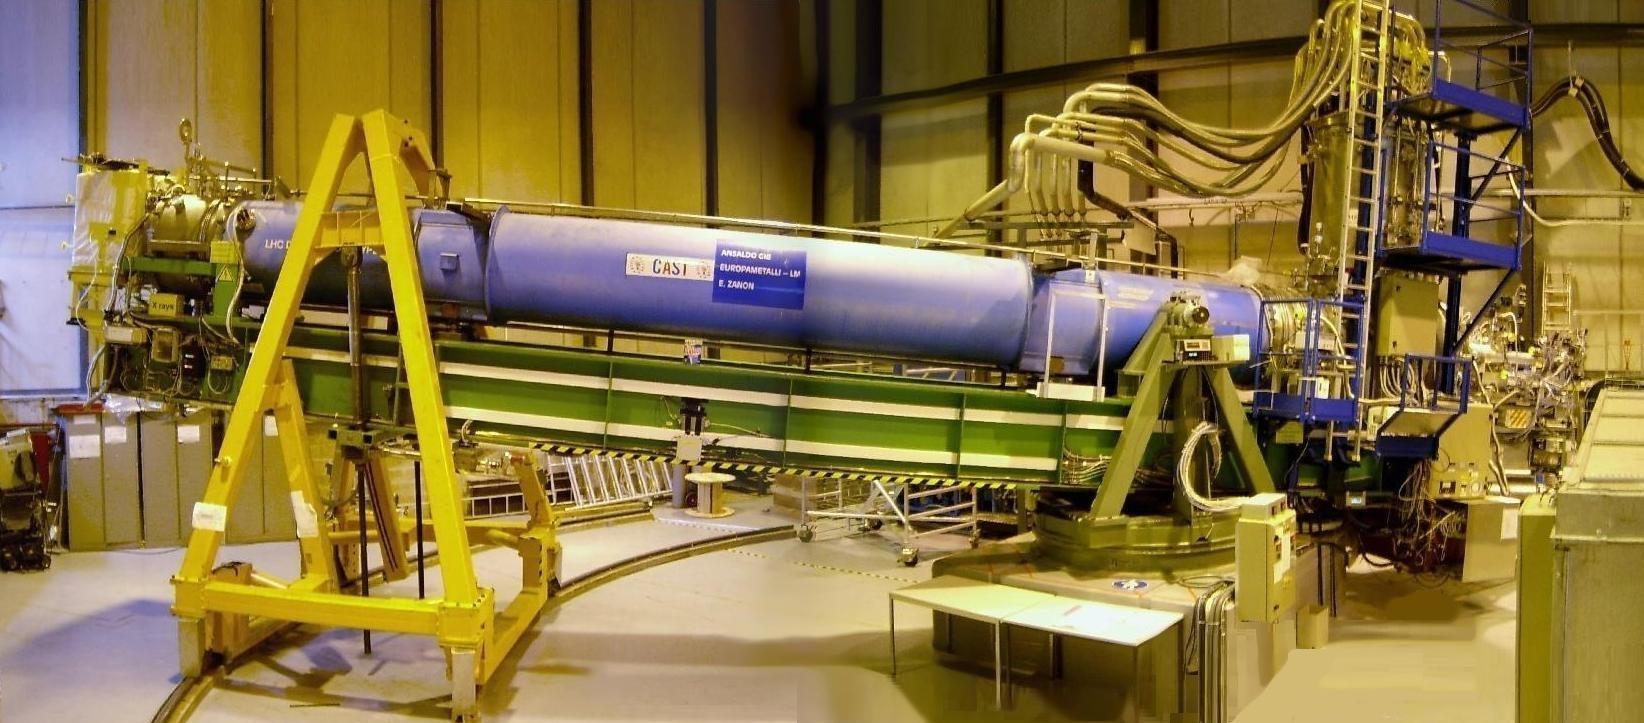
\includegraphics[height=5cm]{figures/cast/cast_instrument.jpg}
  \caption{\footnotesize The Cern Axion Solar Telescope (CAST) located near Geneva, Switzerland. A superconducting ...!!!!!!!!!!!!!!}
  \label{fig:cast_instrument}
\end{figure}

CAST has been doing axion searches since 2002 and the experiment continually improves and reiterates the equipment to get higher sensitivity. One major problem is to get a high enough signal-to-noise ratio, the majority of the noise coming from background radiation from the ground, the materials in the instrument and cosmic rays. The detectors cover the entire area of each bore opening, so are relatively large. Detector size is proportional to the background radiation, so it makes sense to have smaller detectors. By using X-ray optics, the X-ray photons can be focused into a detector area of only a fraction of the previous. This will significantly increase the signal-to-noise ratio and will let the CAST helioscope search for the axion in new areas.

\section{Developing an optic for CAST}
One major concern in making an X-ray optic from NuSTAR glass for the CAST helioscope is the limited space available. The optic would have to fit on the end of the magnet nearest the wall, which leaves only about 2 meters for optic, detector and the focal length between the two. Another problem is the small bore opening of only 43 mm, which is smaller than the inner radius of the NuSTAR telescopes. Both of those problems can be solved by realising that the optic would not require imaging capability and that the axion spectrum is of relatively low energies. In figure \ref{fig:cast_xrt_principle} is seen a top-down view of the end of the magnet bore where the optic and detector can be attached. By stacking a number of reflectors, X-rays can be reflected to one side, something that would not be possible if imaging capabilities were required.

\begin{figure}[htbp]
\centering
\begin{minipage}{.40\textwidth}
  \centering
  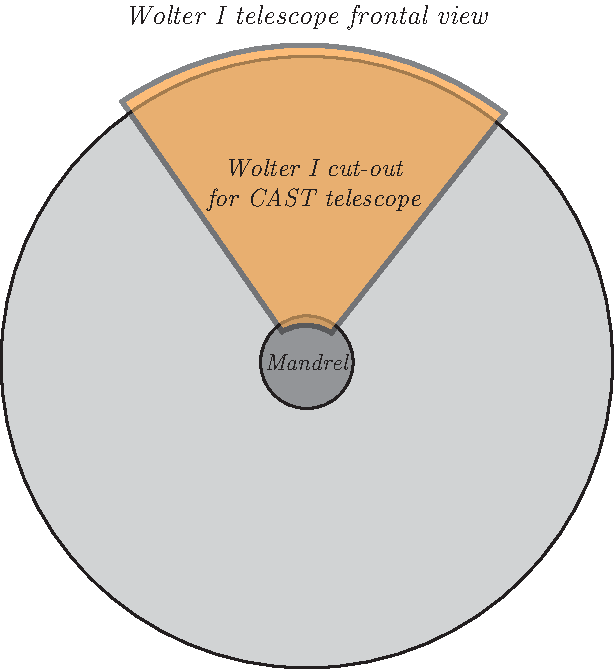
\includegraphics[width=\linewidth]{figures/cast/wolter1-cutout.pdf}
  \captionof{figure}{\footnotesize ront view of Wolter I type optic with section used in the CAST XRT shown.}
  \label{fig:wolter1-cutout}
\end{minipage}%
\hspace{20pt}
\begin{minipage}{.52\textwidth}
  \centering  \includegraphics[width=\linewidth]{figures/cast/cast_xrt_principle.pdf}
  \captionof{figure}{\footnotesize Top-down view of the end of the CAST magnet, where an optic can be attached at one magnet bore. The other magnet bore is taken up by another instrument, resulting in limited space for the CAST XRT.}
  \label{fig:cast_xrt_principle}
\end{minipage}
\end{figure}
% \begin{figure}[htbp]
%   \centering
%     \includegraphics[height=5cm]{figures/cast/wolter1-cutout.pdf}
%     \includegraphics[height=5cm]{figures/cast/cast_xrt_principle.pdf}
%   \caption{\footnotesize Front view of Wolter I type optic with section used in the CAST XRT shown.}
%   \label{fig:wolter1-cutout}
% \end{figure}

By using only 1/6 of the Wolter I radial reflective area, a pie-slice (figure \ref{fig:wolter1-cutout}), two stacks of mirrors can be used to reflect X-rays to one side. The stack only needs to be high enough to cover the bore opening, but each mirror should also be wide enough. The NuSTAR glass pieces are made in 60\degr\ segments for the inner radii and 30\degr\ segments for the outer radii.

\subsection{Optic geometry considerations}
The geometry of the optic was calculated using the following equation for a Wolter I optic:
\begin{eqnarray}\label{eq:wolter}
  \tan(4\alpha) = \frac{\mathit{R3}}{f},
\end{eqnarray}
where $\alpha$ is the angle of reflection of each mirror, $f$ is the focal length and $\mathit{R3}$ is the radius between center of optic and the midpoint between parabolic and hyperbolic mirror (figure \ref{fig:wolter1-diagram}). The center of the bore will need an off-set with the focal plane of the telescope, given by $d = r_{\text{bore}} + r_{\text{min}}$, where $r_{\text{bore}}$ is the radius of the bore and $r_{\text{min}}$ is the minimum radius of a NuSTAR optic. The length of the NuSTAR mirrors is $l = 225$ mm.
% \begin{figure}
% \centering
% \begin{minipage}{.5\textwidth}
%   \centering
%   \includegraphics[width=\linewidth]{figures/cast/wolter1-diagram.eps}
%   \captionof{figure}{Diagram of wolter I from side.R1-R5 designated.}
%   \label{fig:wolter1-diagram}
% \end{minipage}%
% \begin{minipage}{.5\textwidth}
%   \centering  \includegraphics[width=\linewidth]{figures/cast/axion_search_cast.pdf}
%   \captionof{figure}{Show bore-opening with mandrel from front.}
%   \label{fig:optic_and_bore}
% \end{minipage}
% \end{figure}
\begin{figure}[htbp]
  \centering
    \includegraphics[width=0.95\linewidth]{figures/cast/wolter1-diagram.pdf}
  \caption{\footnotesize Diagram of Wolter I from side with $\mathit{R1}$-$\mathit{R5}$ designated. The principle of the Wolter I double reflection can be seen as an X-ray photon is reflected off the parabolic and hyperbolic mirrors. $l$ is mirror length, $f$ is focal length, $x_{sep}$ is distance between parabolic and hyperbolic mirror and $\alpha$ is the angle of reflection for an X-ray photon parallel to the focal plane.}
  \label{fig:wolter1-diagram}
\end{figure}

The focal length $f$ was set to a fixed value of 1.5 m. Using $r_{\text{min}}$ as the 0th layer radius, $\mathit{R3}_0$, the angle of the first layer, $\alpha_0$, can be calculated using eq. \ref{eq:wolter}. From $\alpha_0$ and $\mathit{R3}_0$, we can calculate $\mathit{R1}_0$, $\mathit{R2}_0$, $\mathit{R4}_0$ and \ensuremath{\mathit{R5}_0}:
\begin{eqnarray}
  \mathit{R2}_i &=& \mathit{R3}_i + 0.5\ x_{\text{sep}}\tan(\alpha_i),\\
  \mathit{R1}_i &=& \mathit{R2}_i + l\sin(\alpha_i),\\
  \mathit{R4}_i &=& \mathit{R3}_i - 0.5\ x_{\text{sep}}\tan(3\alpha_i),\\
  \mathit{R5}_i &=& \mathit{R4}_i - l\sin(3\alpha_i),
\end{eqnarray}
for layer $i=0$, where $x_{\text{sep}}$ is the distance between the parabolic and hyperbolic mirror. $\mathit{R4}_1$ and $\mathit{R5}_1$ will be a lower value than $r_{\text{min}}$, so it was nessecary to increase the bore to focal plane distance, $d$.

The next layer can be added by setting $\mathit{R3}_{i+1} = \mathit{R1}_i + d_{\text{glass}}$, where $d_{\text{glass}}$ is the thickness of the glass. Thereby the opening of the next layer will be exactly large enough for all incoming photons to hit the parabolic mirror. All mirror layers are subsequently added using the same method until the stack is high enough to cover the bore opening:
\begin{eqnarray}
  \mathit{R1}_{\text{last}} &\geq& r_{\text{min}} + 2r_{\text{bore}}.
\end{eqnarray}

\begin{figure}[htbp]
\centering
\begin{minipage}{.46\textwidth}
  \centering
  \includegraphics[height=4cm]{figures/cast/cast_front.pdf}
  \captionof{figure}{\footnotesize Computer generated CAST XRT design from front. Black ring designates the magnet bore opening.}
  \label{fig:cast_front}
\end{minipage}%
\hspace{20pt}
\begin{minipage}{.46\textwidth}
  \centering  \includegraphics[width=\linewidth]{figures/cast/cast_side.pdf}
  \captionof{figure}{\footnotesize Computer generated CAST XRT design from side. Magnet bore opening is shown to the left.}
  \label{fig:cast_side}
\end{minipage}
\end{figure}

The calculated geometry can be seen in figure \ref{fig:cast_front} and \ref{fig:cast_side}. The calculated radius and angle for each layer can be seen in table \ref{tab:cast_geometry}. The area is the cross sectional area of the layer opening which overlaps with the magnet bore opening, a description of the calculation can be seen in section \ref{sec:eff_area}.

\begin{table}[!h]
\begin{center}
\begin{tabular}{c|c|c|c|c|c}
Layer & Area [mm$^2$] & $\alpha$ [\degr] & $\alpha$ [mrad] & $\mathit{R1}$ [mm] & $\mathit{R5}$ [mm]\\
\hline
%0&0.000&0.556&9.697&60.500&51.321 \\
1&13.863&0.579&10.113&63.006&53.821 \\
2&48.175&0.603&10.530&65.606&56.043 \\
3&69.270&0.628&10.962&68.305&58.348 \\
4&86.760&0.654&11.411&71.105&60.741 \\
5&102.266&0.680&11.877&74.011&63.223 \\
6&116.172&0.708&12.360&77.027&65.800 \\
7&128.419&0.737&12.861&80.157&68.474 \\
8&138.664&0.767&13.382&83.405&71.249 \\
9&146.281&0.798&13.921&86.775&74.129 \\
10&150.267&0.830&14.481&90.272&77.117 \\
11&149.002&0.863&15.062&93.902&80.218 \\
12&139.621&0.898&15.665&97.668&83.436 \\
13&115.793&0.933&16.290&101.576&86.776 \\
14&47.648&0.970&16.938&105.632&90.241
\end{tabular}
\end{center}
\caption{\footnotesize Geometric properties of the computer generated CAST XRT design. }\label{tab:cast_geometry}
\end{table}

\subsection{Optimising reflective coatings}\label{sec:opt_coatings}
To achieve the maximum possible efficiency of the optic, the coating needed to be optimised for the energy range. In contrast with most astrophysical observatories, the CAST telescope will only look at a single object with a very specific spectrum. That means that the coatings can be tailored to achieve maximum reflectivity in that area of the spectrum. Also known is the quantum efficiency of the detector.

An algorithm was developed to calculate all the different permutations of multilayers for a wide variety of material combinations. The spectrum is at a relatively low X-ray energy, so single layer coatings could be relevant. The algorithm calculates the reflectivity for a multilayer with given material combination and geometry at an angle, $\alpha$, given by the radius of the layer from the optical axis. $F.O.M.$ is then calculated using the following integral:
\begin{equation}\label{eq:fom}
	F.O.M. = \int_{0.1}^{10} \mathbb{R}^2(\mathrm{\alpha},\text{E})\ QE_{\text{det}}(\text{E})\ S_{\text{axion}}(\text{E})\ dE,
\end{equation}
with $\mathbb{R}^2(\mathrm{\alpha},\text{E})$ being the squared reflectivity because of the double reflection, $QE_{\text{det}}(\text{E})$ the detector quantum efficiency and $S_{\text{axion}}(\text{E})$ the axion spectrum as seen in figure \ref{fig:axion_spectrum}. By integrating over the energy range from 0.1 keV to 10 keV, a figure of merit can be obtained that takes both coating, spectrum and detector into account.

The material combinations considered were multilayers of W/B$_4$C, W/Si, Pt/C, Pt/B$_4$C, Ni/B$_4$C as well as single layers of W, Pt, Ir and Ni. W/Si and Pt/C were the most well understood for slumped glass type substrates, since they both were used in the NuSTAR mission. To find the optimal coating, the parameter space considered for each material combination can be seen in table \ref{tab:cast_parameter_space}. By using $d_{\text{min}}$ and $d_{\text{max}}$, both linearly graded-d coatings and constant-d coatings can be computed. To avoid computing cases where \(d_{\text{min}}\) is larger than \(d_{\text{max}}\), the condition \(d_{\text{min}}\) $\leq$ \(d_{\text{max}}\) was set.

\begin{table}[!h]
\begin{center}
\begin{tabular}{c|c|c|c}
Parameter & Minimum & Maximum & Interval \\
\hline
$N$ & 1 layer & 30 layers & 1 layer \\
$d_{\text{min}}$ & 3 nm & 300 nm & 0.5 nm \\
$d_{\text{max}}$ & 3 nm & 300 nm & 0.5 nm \\
$\Gamma$ & 0.1 & 0.9 & 0.05 \\
\end{tabular}
\end{center}
\caption{\footnotesize Parameter space used for finding optimal coating recipes for each material combination.}\label{tab:cast_parameter_space}
\end{table}

For single layer coatings, only a single thickness of 50 nm was considered. The surface and interface roughnesses were fixed at 0.5 nm. The complete computation can be done for every layer in the optic, as $\alpha$ changes throughout the mirror stack. The algorithm does the following steps:
\begin{itemize}
  \item[\bf 1] Finds the next combination in the parameter matrix.
  \item[\bf 2] Calculates the reflectivity using IMD's FRESNEL function.
  \item[\bf 3] Uses the calculated reflectivity in the $F.O.M.$ equation \ref{eq:fom}.
  \item[\bf 4] If the calculated value is higher than the previous maximum value, the parameters are saved and the calculated value set as the new maximum.
\end{itemize}

When the entire parameter space has been covered for a mirror layer and material combination, the algorithm saves the best $F.O.M.$ value and the coating recipe and goes on to the next mirror layer. When all mirror layers are covered, the effective area is calculated whereafter the algorithm continues on to the next material combination.

For the CAST coatings, making a separate coating recipe for each layer would result in having to produce $\sim$14 different coating runs, each with only four mirror substrates. Instead only four different coating recipes were made, where each recipe would be applied to three or four mirror layers. That way 16 mirror substrates could be coated at a time and all substrates could be coated in four coating runs. The result of a full computation using the algorithm with four recipes is shown in figure \ref{fig:mat_result}.

\begin{figure}[htbp]
  \centering
    \includegraphics[height=5cm]{figures/cast/mat_result.pdf}
  \caption{\footnotesize Effective area comparison for computed material combinations in the CAST XRT optic.}
  \label{fig:mat_result}
\end{figure}

The best result for the Pt/C material combination can be seen in figure \ref{fig:pt-c_optimized_recipes}. Curves are the reflectivity squared times detector quantum efficiency times axion spectrum ($\mathbb{R}^2\cdot QE_{\text{det}}\cdot S_{\text{axion}}$) for a given recipe.

\begin{figure}[htbp]
  \centering
    \includegraphics[height=5cm]{figures/cast/pt-c_optimized_recipes1.pdf}
    \includegraphics[height=1.5cm]{figures/cast/pt-c_optimized_recipes2.pdf}
  \caption{\footnotesize Optimised coatings for CAST XRT with a Pt/C material combination. The four recipes are for layer 0-3 (layer 0 is the mandrel), layer 4-7, layer 8-11 and layer 12-14.}
  \label{fig:pt-c_optimized_recipes}
\end{figure}



The coating optimisation for the CAST X-ray optic was done in parallel with most of the ATHENA coating investigations that is described in chapter \ref{chap:athena_coatings}. The findings from long term storage that are discussed in section \ref{sec:long_term} show changes in the coatings over time at ambient conditions for most B$_4$C containing films. For that reason, it was decided to make the CAST coatings with Pt/C, as the combination is well described for NuSTAR like glass substrates. W/Si was also used for NuSTAR and would be a cheaper solution, but the Si absorption line at $\sim2$ keV would decrease efficiency of the coatings around the peak of the axion spectrum.
%Each calculation was done over the energy range $0.1 - 10$ keV with a step size of 0.1 keV.

\subsection{Calculating effective area}\label{sec:eff_area}
The effective area is the cross sectional opening of the optic multiplied by reflectivity squared for each layer. Total effective area is the sum of effective area for each layer:
\begin{eqnarray}
  A_{\text{eff,i}} &=& A_{\text{CS,i}}\mathbb{R}_i^2(\text{E})\\
  A_{\text{eff}} &=& \sum_{i=0}^n A_{\text{eff,i}}
\end{eqnarray}
The cross sectional opening is the intersection of the circle of the bore opening and a layer opening. The layer opening is the cross sectional area between two circles of radius $\mathcal{R}_{i}$ and $\mathcal{R}_{i-1}$, where
\begin{eqnarray}
  \mathcal{R} = \mathit{R1}.
\end{eqnarray}
It can be calculated using the overlap of the outer shell of the layer opening and the bore opening. From that is subtracted the overlap of the inner shell of the layer opening with the bore opening as seen in figure \ref{fig:cross_section_area}.

\begin{figure}[htbp]
  \centering
    \includegraphics[width=0.9\linewidth]{figures/cast/cross_section_area.pdf}
  \caption{\footnotesize Diagram of cross sectional area (CSA) calculation for the intersection of the CAST XRT and CAST magnet bore. \textbf{Left:} CSA of layer $i$ and magnet bore. \textbf{Middle:} CSA of layer $i-1$ and magnet bore. \textbf{Right:} CSA between layer $i$, $i-1$ and magnet bore.}
  \label{fig:cross_section_area}
\end{figure}

Area of the overlap of shell $i$ with bore (figure \ref{fig:cross_section_area} left) is:
\begin{eqnarray}\label{eq:overlap1}
  A_{i} &=& r_{\text{bore}}^2\cos^{-1}\Big(\frac{d^2+r_{\text{bore}}^2-\mathcal{R}_{i}^2}{2dr_{\text{bore}}}\Big)\nonumber\\
  &&+\mathcal{R}_{i}^2\cos^{-1}\Big(\frac{d^2-r_{\text{bore}}^2+\mathcal{R}_{i}^2}{2d\mathcal{R}_{i}^2}\Big)\nonumber\\
  &&-\frac{1}{2}\sqrt{(-d+r_{\text{bore}}+\mathcal{R}_{i})(d+r_{\text{bore}}-\mathcal{R}_{i})}\nonumber\\
  &&\times\sqrt{(d-r_{\text{bore}}+\mathcal{R}_{i})(d+r_{\text{bore}}+\mathcal{R}_{i})},
  %A_{i-1} &=&
\end{eqnarray}
Area of the overlap of shell $i-1$ with bore (figure \ref{fig:cross_section_area} middle) is:
\begin{eqnarray}\label{eq:overlap2}
  A_{i-1} &=& r_{\text{bore}}^2\cos^{-1}\Big(\frac{d^2+r_{\text{bore}}^2-\mathcal{R}_{\text{bot}}^2}{2dr_{\text{bore}}}\Big)\nonumber\\
  &&+\mathcal{R}_{\text{bot}}^2\cos^{-1}\Big(\frac{d^2-r_{\text{bore}}^2+\mathcal{R}_{\text{bot}}^2}{2d\mathcal{R}_{\text{bot}}^2}\Big)\nonumber\\
  &&-\frac{1}{2}\sqrt{(-d+r_{\text{bore}}+\mathcal{R}_{\text{bot}})(d+r_{\text{bore}}-\mathcal{R}_{\text{bot}})}\nonumber\\
  &&\times\sqrt{(d-r_{\text{bore}}+\mathcal{R}_{\text{bot}})(d+r_{\text{bore}}+\mathcal{R}_{\text{bot}})},
\end{eqnarray}
where
\begin{eqnarray}\label{eq:overlap3}
  \mathcal{R}_{\text{bot}} &=& \mathcal{R}_{i-1} + d_{\text{glass}},
\end{eqnarray}
with $\mathcal{R}_{i-1}$ being the radius of the layer underneath layer $i$ and $d_{\text{glass}}$ being the thickness of the glass.

The NuSTAR type telescope is built up from glass layers with graphite spacers between.  Since the optic is so small, but with relatively large openings between the layers, it is necessary to use graphite spacers in the middle. Each of those are rectangular in shape, as high as the opening and $x_{\text{gr}}=2$ mm wide. The spacer obscures the opening, so will have to be subtracted from cross sectional opening. The cross sectional area of the  opening of layer $i$ is then:
\begin{eqnarray}
  A_{\text{CS,i}} &=& A_{i} - A_{i-1} - (\mathcal{R}_{i}-\mathcal{R}_{i-1})x_{\text{gr}}
\end{eqnarray}
The effective area and throughput for the optimised Pt/C coating can be seen in figure \ref{fig:pt-c_effarea_throughput}.

\begin{figure}[htbp]
  \centering
  \includegraphics[width=0.47\linewidth]{figures/cast/pt-c_effara_throughput_lin.pdf}
  \includegraphics[width=0.47\linewidth]{figures/cast/pt-c_effara_throughput_log.pdf}
  \caption{\footnotesize Linear and logarithmic effective area curves of the CAST XRT given in cm$^2$. Throughput is given on the right side of each plot as the fraction of the magnet bore covered by the optic at a given energy.}
  \label{fig:pt-c_effarea_throughput}
\end{figure}

\section{Producing coated substrates}
DTU Space has a fairly large selection of leftover slumped glass substrates from the NuSTAR mission. An extra amount of glass substrates were produced to cover broken pieces and pieces that failed visual inspection. From this surplus, the substrates for the CAST XRT was selected.

\subsection{Collecting substrates for coating}
Each layer for NuSTAR corresponded to a shell diameter, which was described in the serial number of each substrate. The serial number includes diameter and wether it is a parabolic or hyperbolic piece. It is written with a marker on the back of the substrate like the following:
\begin{eqnarray}
  \text{NXXX(A/B)yyy-zzz(s/p),}\nonumber
\end{eqnarray}
where XXX is the diameter of the shell, (A/B)yyy describes the production batch of the slumped glass process, zzz is the layer number of the optic and (s/p) describes wether it is for the first or second stack (parabolic or hyperbolic). Since the NuSTAR optic is a conical approximation to the Wolter I geometry, the glass substrates are conical in shape. So instead of being parabolic or hyperbolic, they are straight along the optical axis.

To find pieces for the CAST XRT, the diameter described by XXX would need to correspond with the calculated $\mathit{R1}$ and $\mathit{R2}$ values for the first piece, or $\mathit{R4}$ and $\mathit{R5}$ for the second piece. The pieces should be mounted at higher grazing incidence angles than NuSTAR, so the difference between $\mathit{R1}$ and $\mathit{R2}$ are higher for CAST than NuSTAR. That difference would need to be corrected for by bending each piece to the correct shape during the mounting process. The NuSTAR pieces corresponding to the CAST radii can be seen in table \ref{tab:cast_pieces}.

\begin{table}[p]
\begin{center}
\begin{tabular}{c|c|c|c|c}
Layer & Mean diam. & Corresp. & Mean diam. & Corresp. \\
& (parabolic)  & NuSTAR & (hyperbolic)  & NuSTAR  \\
& [mm] &  diam. [mm] & [mm] &  diam. [mm]\\
\hline
1&124.2&124&114.7&116\\
2&129.3&128&119.5&120\\
3&134.7&136&124.4&124\\
4&140.3&140&129.6&128\\
5&146.0&144&134.9&136\\
6&152.0&152&140.5&140\\
7&158.3&160&146.2&148\\
8&164.8&164&152.2&152\\
9&172.5&172&158.4&160\\
10&178.4&180&164.8&164\\
11&185.7&184&171.5&172\\
12&193.2&192&178.5&180\\
13&201.0&200&185.7&184\\
14&209.1&208&193.1&192
\end{tabular}
\end{center}
\caption{\footnotesize Table of radii of each layer for the parabolic and hyperbolic mirrors in the CAST XRT compared to compatible NuSTAR radii.}\label{tab:cast_pieces}
\end{table}

\begin{figure}[htbp]
  \centering  \includegraphics[height=6cm]{figures/cast/pieces_for_cleaning.jpg}
  \caption{\footnotesize Glass substrates selected for the CAST XRT before cleaning. The substrates required for each recipe were collected in four different baskets.}
  \label{fig:pieces_for_cleaning}
\end{figure}

With 14 glass layers and two stacks, 28 pieces are needed for the CAST XRT optic. As the glass pieces are very fragile and tend to break, it was decided to produce twice the amount, 56 in total.

Each piece was visually inspected and the best pieces were selected for the CAST XRT (figure \ref{fig:pieces_for_cleaning}). The pieces were subsequently cleaned by the following process:
\begin{enumerate}
  \item Ethanol rinsing to clear away markers.
  \item Clean room wipes were used to remove visible blemishes.\label{item:clean_wipes}
  \item 15 min. in ultrasonic bath with milli-Q water and soap (figure \ref{fig:cast_cleaning_soap}).
  \item Thorough rinse with milli-Q water to remove soap.
  \item 15 min. in ultrasonic acetone bath (figure \ref{fig:cast_cleaning_ethanol}).
  \item 15 min. in ethanol bath (figure \ref{fig:cast_cleaning_ethanol}).
  \item Each piece rinsed with milli-Q water and carefully dried with dry N$_2$.
  \item Visual inspection, if failed, repeat from step \ref{item:clean_wipes}.
\end{enumerate}

\begin{figure}[htbp]
\centering
\begin{minipage}{.46\textwidth}
  \centering
  \includegraphics[height=4.5cm,trim= 0 100 0 200,clip]{figures/cast/soap_bath.jpg}
  \captionof{figure}{\footnotesize Ultra-sonic bath with soap.}
  \label{fig:cast_cleaning_soap}
\end{minipage}%
\hspace{20pt}
\begin{minipage}{.46\textwidth}
  \centering
  \includegraphics[width=0.9\linewidth]{figures/cast/acetone_and_ethanol.jpg}
  \captionof{figure}{\footnotesize Acetone and ethanol tubs. \textbf{Left:} Acetone tub in ultra-sonic machine. \textbf{Right:} Ethanol tub.}
  \label{fig:cast_cleaning_ethanol}
\end{minipage}
\end{figure}

The pieces were moved directly to sample mounting plates (figure \ref{fig:coating_mount}) in a downflow module to avoid dust contamination.

\begin{figure}[htbp]
  \centering
    \includegraphics[height=6cm]{figures/cast/coating_mount.jpg}
  \caption{\footnotesize Cleaned glass substrates attached to sample mounting plate before coating. Two glass substrates were mounted onto each plate at positions 25 cm and 35 cm above coating chamber floor.}
  \label{fig:coating_mount}
\end{figure}

\subsection{Coating of substrates}
Four coating recipes were made for the CAST XRT. With 56 pieces to coat, 12-16 pieces are needed per recipe. The  coating chamber in the DTU Space multilab can hold up to 36 substrates if the entire length of each cathode is utilized. To ensure a uniform coating, only the center part of the coating cathodes are used. Two substrates were mounted on each plate so the center of each sample was 25 cm or 35 cm above the chamber floor. Along with the glass substrates, two Si wafer pieces were installed on a separate plate at the same height to become witness samples.

From the coating optimisation calculations described in section \ref{sec:opt_coatings}, the optimal material combination was chosen to be Pt/C. Before coating, a thorough calibration was needed, which was done as described in section \ref{sec:coating_calib}. Honeycomb (6.4 mm opening, 5 mm thickness) was used as collimation in front of the cathodes. A Pt target was mounted in cathode 2 and a 2-piece C target was mounted in cathode 4. Power settings were 450 W for cathode 2 and 900 W for cathode 4. Ar was supplied to the chamber at 88 SCCM, corresponding to a coating pressure of 2.9 mTorr. Background pressure for each coating was $\leq 2\cdot10^{-6}$ Torr.

\begin{figure}[htbp]
  \centering
    \includegraphics[height=7cm]{figures/cast/coated_pieces.jpg}
  \caption{\footnotesize Mounted glass substrates in coating chamber after coating. }
  \label{fig:coated_pieces}
\end{figure}

In figure \ref{fig:coated_pieces} can be seen the glass substrates after a coating still mounted in the coating chamber.

The coating was done with each material separately. With all cathodes turned off and the ring at the position where the first sample plate is between cathode 1 and 4, the ring would first move so sample plate 1 is next to the cathode of the first material. The cathode would then turn on, the shutter open and the ring start moving at the speed obtained from calibration corresponding to the thickness found in section \ref{sec:opt_coatings}. After one full rotation, the shutter closes, the cathode turns off and the ring returns to the start position before starting on the next material.

The power supplies were polled every 5 seconds to get the power output, which can be seen in figure \ref{fig:cast_coatings_power} for the coatings of recipe 1 and recipe 4. Cathode 5 and 6 are actually cathode 3 and 4 in the chamber, but are run from a third dual channel power supply. During the recipe 4 coatings can be seen some fluctuations in the cathode 4 power output, they are caused by the  instabilities that occur when coating with non-metallic materials at high power.

\begin{figure}[htbp]
  \centering  \includegraphics[width=0.45\linewidth]{figures/cast/power_recipe1.pdf}  \includegraphics[width=0.45\linewidth]{figures/cast/power_recipe4.pdf}\\
  \caption{\footnotesize Graphs of power output delivered to cathodes from power supplies during CAST XRT multilayer coatings. \textbf{Left:} Cathode power output during recipe 1 coatings, two bilayers. \textbf{Right:} Cathode power output during recipe 4 coatings, five bilayers.}
  \label{fig:cast_coatings_power}
\end{figure}

The Si witness samples were measured at the XRR lab at DTU Space. XRR results from each witness sample for recipes 1-4 can be seen in figure \ref{fig:cast_recipe_xrr}. In each of the four coating runs, the two witness samples show completely similar XRR structure indicating a high uniformity between the two sample mounting positions. An exception is the witness samples from recipe 2, which show shifted peaks especially at higher angles as well as dissimilarities around the 5th peak.

\begin{figure}[htbp]
  \centering  \includegraphics[width=0.45\linewidth]{figures/cast/cast_recipe1.pdf}  \includegraphics[width=0.45\linewidth]{figures/cast/cast_recipe2.pdf}\\  \includegraphics[width=0.45\linewidth]{figures/cast/cast_recipe3.pdf}  \includegraphics[width=0.45\linewidth]{figures/cast/cast_recipe4.pdf}
  \caption{\footnotesize XRR measurements of witness samples from CAST XRT coatings recipe 1-4. Each coating run included two witness samples placed at 25 cm and 35 cm above coating chamber floor, same as glass substrates.}
  \label{fig:cast_recipe_xrr}
\end{figure}

XRR data of witness samples were compared to an IMD model as seen in figures \ref{fig:cast_fit_rec1}, \ref{fig:cast_fit_rec2-1}, \ref{fig:cast_fit_rec2-2}, \ref{fig:cast_fit_rec3} and \ref{fig:cast_fit_rec4}. All fits show good agreement with XRR measurements despite the difficulties in fitting graded-d coatings as each layer thickness and interface roughness is an independent variable.

\begin{figure}[h!]
\centering
\begin{minipage}{.47\textwidth}
  \centering
  \includegraphics[width=\linewidth]{figures/cast/cast_recipe1_fit.pdf}
\end{minipage}%
\begin{minipage}{.53\textwidth}
  \centering
  \footnotesize
  \begin{tabular}{c|c|c|c|c}

i&d$_{\text{aim}}$ [nm]&$\Gamma_{\text{aim}}$&d$_{\text{fit}}$ [nm]&$\Gamma_{\text{fit}}$\\
  \hline
  1&22.5&0.45&22.48&0.462\\
  2&11.5&0.45&11.19&0.462
  \end{tabular}
\end{minipage}
\caption{\footnotesize XRR measurement of witness sample from CAST XRT recipe 1 coating compared to IMD model fit.}\label{fig:cast_fit_rec1}
\end{figure}

\begin{figure}[h!]
\centering
\begin{minipage}{.47\textwidth}
  \centering
  \includegraphics[width=\linewidth]{figures/cast/cast_recipe2_fit1.pdf}
\end{minipage}%
\begin{minipage}{.53\textwidth}
  \centering
  \footnotesize
  \begin{tabular}{c|c|c|c|c}
  i&d$_{\text{aim}}$ [nm]&$\Gamma_{\text{aim}}$&d$_{\text{fit}}$ [nm]&$\Gamma_{\text{fit}}$\\
  \hline
  1&19&0.45&18.53&0.46\\
  2&13&0.45&13.93&0.54\\
  3&7&0.45&6.89&0.46
  \end{tabular}
\end{minipage}
\caption{\footnotesize XRR measurement of witness sample from CAST XRT recipe 2 coating compared to IMD model fit. Witness sample was mounted 35 cm above coating chamber floor.}\label{fig:cast_fit_rec2-1}
\end{figure}

\begin{figure}[h!]
\centering
\begin{minipage}{.47\textwidth}
  \centering
  \includegraphics[width=\linewidth]{figures/cast/cast_recipe2_fit2.pdf}
\end{minipage}%
\begin{minipage}{.53\textwidth}
  \centering
  \footnotesize
\begin{tabular}{c|c|c|c|c}
i&d$_{\text{aim}}$ [nm]&$\Gamma_{\text{aim}}$&d$_{\text{fit}}$ [nm]&$\Gamma_{\text{fit}}$\\
\hline
1&19&0.45&18.40&0.448\\
2&13&0.45&14.57&0.558\\
3&7&0.45&6.99&0.449
\end{tabular}
\end{minipage}
\caption{\footnotesize XRR measurement of witness sample from CAST XRT recipe 2 coating compared to IMD model fit. Witness sample was mounted 25 cm above coating chamber floor.}\label{fig:cast_fit_rec2-2}
\end{figure}

\begin{figure}[h!]
\centering
\begin{minipage}{.47\textwidth}
  \centering
  \includegraphics[width=\linewidth]{figures/cast/cast_recipe3_fit.pdf}
\end{minipage}%
\begin{minipage}{.53\textwidth}
  \centering
  \footnotesize
\begin{tabular}{c|c|c|c|c}
i&d$_{\text{aim}}$ [nm]&$\Gamma_{\text{aim}}$&d$_{\text{fit}}$ [nm]&$\Gamma_{\text{fit}}$\\
\hline
1&16&0.4&16.19&0.411\\
2&12.5&0.4&12.27&0.394\\
3&9&0.4&9.04&0.386\\
4&5.5&0.4&5.17&0.440
\end{tabular}
\end{minipage}
\caption{\footnotesize XRR measurement of witness sample from CAST XRT recipe 3 coating compared to IMD model fit.}\label{fig:cast_fit_rec3}
\end{figure}

\begin{figure}[h!]
\centering
\begin{minipage}{.47\textwidth}
  \centering
  \includegraphics[width=\linewidth]{figures/cast/cast_recipe4_fit.pdf}
\end{minipage}%
\begin{minipage}{.53\textwidth}
  \centering
  \footnotesize
\begin{tabular}{c|c|c|c|c}
i&d$_{\text{aim}}$ [nm]&$\Gamma_{\text{aim}}$&d$_{\text{fit}}$ [nm]&$\Gamma_{\text{fit}}$\\
\hline
1&14&0.4&13.61&0.397\\
2&11.75&0.4&11.44&0.400\\
3&9.5&0.4&9.27&0.404\\
4&7.25&0.4&7.10&0.408\\
5&5&0.4&4.93&0.412
\end{tabular}
\end{minipage}
\caption{\footnotesize XRR measurement of witness sample from CAST XRT recipe 4 coating compared to IMD model fit.}\label{fig:cast_fit_rec4}
\end{figure}

Both top and bottom witness sample from the recipe 2 coatings were fitted given the dissimilarities stated above. The targeted coating for recipe 2 were 3 layers with d$_{\text{min}}=7$ nm, d$_{\text{max}}=19$ nm, $\Gamma=0.45$. Both top and bottom witness sample show a significant irregularity in the second bilayer where $\Gamma \simeq 0.55$ and d $\simeq$ 13.93-14.57 nm. The results warranted a thorough check of coating log and the coating macro used for the coating, as the irregularities could be at least partly explained by an error in the coating macro. No sign of error in the calculations of the coating macro, and the coating log also revealed that the speeds used during the coating corresponded to the values obtained in the calibration.

\begin{table}
  \centering
\begin{tabular}{c|c|c|c|c}
Witn. sample& d-C$_{\text{aim}}$ [nm]&d-C$_{\text{fit}}$ [nm]&d-Pt$_{\text{aim}}$ [nm]&d-Pt$_{\text{fit}}$ [nm]\\
\hline
Top&5.85&7.52&7.15&6.41\\
Bottom&5.85&8.13&7.15&6.44\\
\end{tabular}
\caption{\footnotesize Thicknesses of CAST XRT recipe 2 layer 2 in top and bottom witness sample, designed d-spacings from recipe compared to d-spacings obtained from XRR measurement and IMD fitting.}\label{tab:recipe2layer2}
\end{table}

The d-spacings for the second layer in recipe 2 compared to IMD fits of XRR data from top and bottom witness sample are shown in table \ref{tab:recipe2layer2}. An explanation for the inconsistencies between top and bottom witness sample could be problems with a cathode during coating. Column 3 shows inconsistencies between top and bottom witness sample in the C thickness, but it is not seen in the Pt thickness, column 5. That corroborates the hypothesis that the C cathode had difficulties during the application of the second layer, as indeed can be seen in figure \ref{fig:cast_coatings_power_recipe2_layer2}. The cathode is only polled every 5 seconds, so intermittent dropouts between polling are likely to have occurred. Top and bottom witness sample were mounted on the same plate, so passed the cathode simultaneously. The difference in C thickness can only be explained by a non-uniform coating rate of C during the coating of layer 2. A partial dropout of the C cathode could have put the power supply in a state where to reignite the plasma, the cathode would for some time have a non-uniform plasma density. Another explanation could be a localized charge-up on the C target during coating caused by the insulating properties of the material \footnote{The carbon targets used at DTU Space are boron-doped to increase the conductivity of the bulk material.}. Such a charge-up would change the electric field in front of the target and thereby create a non-uniform plasma density.

\begin{figure}[htbp]
  \centering  \includegraphics[width=0.7\linewidth]{figures/cast/power_cat6.png}
  \caption{\footnotesize Power output delivered to cathode 6 (carbon) during coating of layer 2, recipe 2. }
  \label{fig:cast_coatings_power_recipe2_layer2}
\end{figure}

The drop-outs of the C cathode can only explain the difference in C thickness between top and bottom witness sample. The inconsistencies of layer 2, recipe 2 is at the time of writing still of unknown origin.

The coated substrates were packed and shipped to LLNL for assembly.

\emph{The substrates were shipped with DHL, but the package was lost between Denmark and the US. A new batch of substrates were collected, cleaned, coated, packed and shipped during June/July of 2014. In this chapter is described the process for the second batch.}

\section{Assembling coated substrates}
Optic assembly was carried out at LLNL, where one of the NuSTAR assembly machines were set up for that purpose. The machine had been adjusted to make only a 30\degr\ section of substrates, and a specially designed Ti mandrel had been procured.

\begin{figure}[htbp]
  \centering
  \includegraphics[width=0.45\linewidth]{figures/cast/assembly1.jpg}
  \includegraphics[width=0.45\linewidth]{figures/cast/assembly2.jpg}
  \caption{\footnotesize Pictures of glass substrates mounted on Ti mandrel during assembly. Three graphite spacers are attached on top of each glass substrate and machined to correct thickness before mounting of the next substrate.}
  \label{fig:cast_assembly}
\end{figure}

Three graphite spacers were mounted onto the mandrel with epoxy glue and machined to the correct thickness before the two pieces for the first layer were mounted, again using epoxy. The next set of graphite spacers were mounted onto the first glass substrates and then machined to the right thickness (figure \ref{fig:cast_assembly}).

\subsection{Vacuum vessel}
The magnet bores and detectors in the CAST helioscope operates at vacuum levels, so the entire optic had to be mounted inside a vacuum vessel. To align the optic after mounting it on the CAST helioscope, it was necessary to have linear actuators for the translation and rotation of the optic while under vacuum.

\begin{figure}[htbp]
  \centering
    \includegraphics[width=0.45\linewidth]{figures/cast/cast_vessel1.jpg}
    \includegraphics[width=0.45\linewidth]{figures/cast/cast_vessel2.jpg}
  \caption{\footnotesize Vacuum vessel for the CAST XRT. \textbf{Left:} Vacuum vessel with linear actuators and guide rods viewable. CF flange is mounted directly to the magnet. \textbf{Right:} Inside of vacuum vessel as viewed from CF flange. A metal plate with two openings cover the graphite spacers in the center between the glass layers. }
  \label{fig:cast_vessel}
\end{figure}

The vacuum vessel can be seen in figure \ref{fig:cast_vessel}. It was designed by Todd Decker (also pictured), an engineer from LLNL. In the picture can be seen five linear actuators, two on top to control pitch, three on the side, one for translation and two for yaw control. The three metal rods also visible on the side are for sliding out the optic, to make a precise optical alignment using a theodolite, described in detail in section \ref{sec:optic_alignment}.

Because of the limited space at the place where the optic had to be installed and the method of which to align it, the number of layers were cut from 14 to 13 layers. With 14 layers, the freedom of movement of the optic inside the vacuum vessel would have been severely limited and possibly caused the optic to hit the vacuum vessel wall during alignment.

\section{Installation of optic at CAST}
The optic mounted in the vacuum vessel was shipped to CERN for installation in Aug. 2014. The vessel was leak tested with He before being lifted into position in front of the magnet bore using a crane as seen in figure \ref{fig:cast_install}.

\begin{figure}[htbp]
  \centering
    \includegraphics[height=6cm]{figures/cast/castxrt_install.jpg}
  \caption{\footnotesize The vacuum vessel housing the CAST XRT is lowered into place at the end of the CAST magnet using a crane.}
  \label{fig:cast_install}
\end{figure}

After mounting, vacuum view ports were mounted at either end of the magnet bores, making it possible to shine a laser straight through into the optic from the other end. The entire helioscope and magnet bore were also precisely aligned with a theodolite.

\subsection{Optic alignment}\label{sec:optic_alignment}
Inside the vacuum vessel, specially designed metal pieces were mounted to either end of the mandrel, one piece can be seen in figure \ref{fig:cast_vessel} (right). They have openings to allow photons into the optic and a narrow piece in the middle that blocks the graphite spacers between the glass pieces. Just above the top layer of glass was made a small hole in one of the metal pieces and on the other was mounted a small metal ball. The ball and hole were at the same distance from the center of the optic. The side of the vacuum vessel was designed so it could slide out a short distance along three precisely machined rods. By setting a pair of premachined spacers in the opening, the distance that the optic has slid out is exactly the distance from the hole and ball and the center of the optic.

A theodolite mounted 3 m from the front of the helioscope was aligned with the bore axis, so looking through the theodolite one could see the ball and hole of the optic. The optic rotation and translation could then be adjusted using the linear actuators to line up the ball and hole, and get a precise alignment. The theodolite could be set to shine a laser beam with adjustable divergence through the bore and at the optic. The view from the detector side can be seen in figure \ref{fig:ball_and_hole}. After the hole and ball was lined up, the optic was slid back into the vacuum vessel and the bolts were fastened.

\begin{figure}[htbp]
  \centering
    \includegraphics[height=4cm,trim=40 10 60 0, clip]{figures/cast/ballandhole.pdf}
    %\hspace{20pt}
    \includegraphics[width=0.47\linewidth]{figures/cast/ballandhole.jpg}
  \caption{\footnotesize \textbf{Left:} Picture taken from the detector side of the CAST XRT as a divergent laser beam shines through. A piece of paper covers the opening and is lit up by the laser. The optic has been moved out for alignment and the ball and hole are visible above the top glass layer. \textbf{Right:} CAD drawing of the CAST XRT with end-plates showing the ball and hole of the gunsight used for alignment (from Todd Decker, LLNL). }
  \label{fig:ball_and_hole}
\end{figure}

The optic reflected the laser light nicely, making it possible to get an exact position for the detector as seen in figure \ref{fig:cast_align} (left). A fake detector with a carbonite back was used for the alignment. That allowed the laser light focused by the optic to shine at the carbonite back and be viewable from the other side.

\begin{figure}[htbp]
  \centering
    \includegraphics[height=5cm]{figures/cast/castxrt_alignment1.jpg}
    \hspace{20pt}
    \includegraphics[width=0.45\linewidth]{figures/cast/castxrt_alignment2.jpg}
  \caption{\footnotesize MicroMegas detector alignment. \textbf{Left:} A fake detector with a carbonite back was installed. The divergent laser beam focused to a spot by the X-ray optic can be seen through the carbonite back. \textbf{Right:} The fake detector was exchanged for a functioning MicroMegas detector in the same mounting bracket and was connected to the vacuum system with XRT and magnet.}
  \label{fig:cast_align}
\end{figure}

The position of the detector was adjusted to make the spot hit in exactly the center. The detector mounts could then be fastened and the fake detector could then be replaced by a real one as seen in figure \ref{fig:cast_align} (right).

\subsection{Tests with 8 keV X-ray source}
The last task with detector and optic in place was a test with X-rays. An X-ray souce had to be mounted in front of the helioscope, but still under vacuum. It was decided to use a COOL-X pyroelectric X-ray source. It works by warming and cooling a pyroelectric element, which emits electrons that subsequently hits a Cu target and an X-ray spectrum gets emitted with a peak at the Cu K$_{\alpha_1}$ energy. The source has a flux of $10^8$ photons/sec. emitted at an angle of 160\degr, so at a distance of $\sim$14.2 m from the optic, $<10$ photons/sec. would arrive at the detector on average given then effectivity of the optic at $\sim$8 keV, detector efficiency and the non-constant flux from the source.

% \begin{figure}[htbp]
%   \centering
%     \includegraphics[width=0.47\linewidth,trim=40pt 0pt 30pt 0]{figures/cast/cast_5h_1000x.png}
%     \includegraphics[width=0.47\linewidth,trim=40pt 0pt 30pt 0]{figures/cast/cast_5h_200x.png}
%   \caption{\footnotesize }
%   \label{fig:cast_5h_run}
% \end{figure}

%In figure \ref{fig:cast_5h_run} can be seen the data output from the MicroMegas detectors after a 5 hour measurement with the COOL-X X-ray source. Left figure is exact positions of each photon hitting the detector, right side shows the photons collected into bins, 200 bins per axis. The spot is $\sim$7 mm long and $\sim$5 mm wide, the relatively large spot is expected since the source is not a point source infinitely far away.
%A flux of less than 1 Hz was seen in the spot. According to the effective area plot in figure \ref{fig:pt-c_effarea_throughput}, the throughput at 8 keV is only $\sim$1\%.

Ray-tracing was done by Michael J. Pivovaroff from LLNL, and can be seen in figure \ref{fig:raytracing1}. The simulations assumes a 6 mm diameter source placed 14.2 m from the optic and glass figure errors comparable to the NuSTAR optic. The MicroMegas data from the 5 hour measurement was rotated 45 degrees and binned into 200 x 200 $\upmu$m$^2$ virtual pixels. By ray-tracing a 6 mm spot at discrete photon energies from 0-10 keV and using the measured spectrum as weight, a composite image was created to compare with measured data. The left plot of figure \ref{fig:raytracing1} is the ray-tracing and the right is the measured data with the ray-tracing model shown as red lines.

\begin{figure}[htbp]
  \centering
    \includegraphics[width=0.47\linewidth]{figures/cast/coolX-simulation.pdf}
    \includegraphics[width=0.47\linewidth]{figures/cast/coolX-SRMM.pdf}
  \caption{\footnotesize Comparison of ray-trace model with measurement using the COOL-X X-ray source.  \textbf{Left:} Ray-tracing simulation considering a 6 mm source 14.2 m from the optic.  \textbf{Right:} Measurement over 5 hours using the COOL-X X-ray source. White contours are from ray-tracing simulation. (From Michael J. Pivovaroff, LLNL) }
  \label{fig:raytracing1}
\end{figure}

Using the same model, a ray-tracing was done using a 3' source to mimic the helioscope looking at the sun and having axions converted into X-rays in the magnet. In figure \ref{fig:raytracing2} can be seen two ray-tracing models with a 3' source. Left plot assumes optic figure error of 1' (similar to NuSTAR) and right plot assumes optic figure error of 1.3'.

\begin{figure}[htbp]
  \centering
    \includegraphics[width=0.47\linewidth]{figures/cast/sunspot10.pdf}
    \includegraphics[width=0.47\linewidth]{figures/cast/sunspot13.pdf}
  \caption{\footnotesize Ray-trace model of CAST XRT considering the sun as a 3' source.  \textbf{Left:} Ray-tracing simulation considering optic with a figure error similar to NuSTAR of $\sim$1'.  \textbf{Right:} Ray-tracing simulation considering optic with a figure error 1.3 times greater than for NuSTAR ($\sim$1.3'). (From Michael J. Pivovaroff, LLNL) }
  \label{fig:raytracing2}
\end{figure}

The ray-tracing models show a half-power area of 8.6 mm$^2$ for the COOL-X X-ray source simulation , which corresponds well with the measurements seen in figure \ref{fig:raytracing1} (right). The measurements only lasted for 5 hours, so the photon count was relatively small because of the low flux from the source that actually reached the optic. The ray-tracing for a 3' source mimicking the sun show a half-power area of 1.44 mm$^2$. Had the optic figure been perfect (0'), the half-power area would be 1.39 mm$^2$, so the CAST XRT is close to the optimal performance.

In figure \ref{fig:raytracing3} can be seen the ray-tracing model computed for the as-designed multilayer coating (fig. \ref{fig:pt-c_optimized_recipes}) compared to the actual XRR measured and fitted multilayer coating (figures \ref{fig:cast_fit_rec1}--\ref{fig:cast_fit_rec4}). The as-coated multilayers differ in reflectivity response from as-designed multilayers by up to 0.5\% at the higher energies, at mid and lower energies the difference is less than 0.1\%. At higher energies, the effective area of the CAST XRT is  $< 10^{-1}$ cm$^2$ so changes in effective area become more pronounced.

\begin{figure}[htbp]
  \centering
    \includegraphics[width=0.47\linewidth]{figures/cast/raytracing_diff_cm2.pdf}
    \includegraphics[width=0.47\linewidth]{figures/cast/raytracing_diff_perc.pdf}
  \caption{\footnotesize Difference in the ray-trace model between as-designed multilayer coatings and actual XRR measured and fitted multilayer coatings.  \textbf{Left:} Difference in cm$^2$. \textbf{Right:} Difference in \% from actual effective area. (From Michael J. Pivovaroff, LLNL) }
  \label{fig:raytracing3}
\end{figure}

\section{Conclusion}
In this chapter was shown the creation of an X-ray optic from design phase to installation. The whole process was $\sim$2 years from start to finish and realised on a minimal budget with surplus materials and instrumentation where possible.

The measurement results obtained using the COOL-X X-ray source combined with ray-tracing simulations, show that surplus slumped glass can be re-purposed into well-behaving X-ray optics for specialised tasks.

It was shown that a customised software solution interfacing to IMD can find the optimal geometry for a specific X-ray optic and make comparisons of best recipe material combinations. The specially designed software can make a full computation with a wide range of material combinations and multilayer coating geometries within 2-3 days using a regular desktop computer. Using a calculation of the overlap between optic opening and magnetic bore opening, a precise effective area can be calculated with the software.

A discussion of possible improvements in the software can be found in the following section.

\subsection{Improvements to the software}\label{sec:software_improvements}
The software is limited by the inability of IMD to use more than one core on common multi-core CPUs that is found in most computers today. The limit can be circumvented by letting the software spawn an instance of IMD for every processor core. That could be done by separating the calculations of each recipe, so e.g. four cores can calculate four recipes at the same time. The challenge is however to let each subprocess return the calculated optimised recipes without interrupting another subprocess. It would also require the same number of IDL instances run at the same time on one computer. This can be done using the Python \verb|subprocess.Popen| class. An example is given here. The first Python script imports the Popen procedure and spawns an instance of Popen that opens the file \verb|subp.py| in Python and that is called \verb|process1|. Popen can be set to pipe back output from \verb|process1|, but that will make the script wait for the output from the first instance before spawning the second instance called \verb|proces2|. This script will simply open subp.py in two separate instances of Python and then quit.

\begin{verbcode}
from subprocess import Popen

process1 = Popen(['python', 'subp.py', '-d'])

process2 = Popen(['python', 'subp.py', '-d'])
\end{verbcode}

The contents of \verb|subp.py| can be seen below. It imports \verb|pidly|, which is a class that facilitates communication between Python and IDL. It then spawns an instance of Pidly called \verb|idl| (that also opens IDL), and using the \verb|idl| instance, commands can be piped directly into the IDL application. It can also run IDL procedures (\verb|*.pro|-files) or start an IMD terminal in that instance (\verb|.r IMD|).

\begin{verbcode}
import pidly

idl = pidly.IDL()
idl('for i=0, 100000 do begin & a=sqrt(i/255)')
\end{verbcode}

The example given above will use 100\% of two cores in a multi-core CPU, and is a very simplistic form of multi threading. The output from each instance of IDL can be written to files on the hard drive and read by the main Python program when the IDL computation is done. That can be done in a brute force manner by simply letting the main Python program wait until the number of IDL instances running on the computer is zero. That works well if each computation takes roughly the same time, but a more advanced approach can be taken in other cases, where Python will open a new process whenever a CPU core becomes available. The two Linux Bash commands below will get the number of CPU cores in the system and the number of IDL instances running, respectively. The second line will also count itself as a program running that is called something with \verb|idl| in the name, which should be accounted for.

\begin{verbcode}
  $ cat /proc/cpuinfo | grep -c cpuid

  $ ps a | grep -c idl
\end{verbcode}

In codebases where new instances of \verb|Popen| are spawned rapidly and output files are read in between, the main process should run on its own CPU core. Otherwise a bottleneck will occur where the main program is slowed by subprocesses taking over system resources and new subprocesses will not be spawned fast enough.

Apart from speed improvements, the software is made with lower energy X-ray optics in mind. Specifically, it is limited to linearly graded multilayers, where for higher energy (10+ keV X-rays) the optimal choice would be a power-law grading. In that case, the variables to optimise would be $a$, $b$, and $c$ in the power law $d_i = a/(b+i)^c$ and the number of layers, $N$.

\chapter{Telescope design for the International AXion Observatory (IAXO)}\label{chap:iaxo}

CAST is a third generation axion helioscope and was the first experiment to surpass the astrophysical limit on the axion-photon coupling of \gay\ $\lesssim 10^{10}$ Gev$^{-1}$ in a broad axion mass range. The CAST helioscope search has reached slightly into the part of parameter space predicted by models to be most likely to detect the axion.

To improve on the CAST achievements and reach further into the "axion band" of the parameter space, a more sensitive instrument is required.

\section{IAXO concept}
Considering that the probability of converting a solar axion into a photon in a magnet with magnetic field $B$ and length $L$ is given by\cite{Andriamonje:2007jc,Zioutas:2005jl,Sikivie:1983wx}:

\begin{eqnarray}
  P_{\text{a}\gamma} &=& 2.6\cdot10^{-17}\bigg(\frac{B}{10\text{ T}}\bigg)^2\bigg(\frac{L}{10\text{ m}}\bigg)^2(g_{\text{a}\gamma}\cdot10^{10}\text{\ GeV})^2\mathcal{F},
\end{eqnarray}

where $\mathcal{F}$ is the coherence length:

\begin{eqnarray}
  \mathcal{F} &=& \frac{2(1-\cos{qL})}{(qL)^2}
\end{eqnarray}

and $q$ is the momentum transfer. It becomes apparent that in order to improve on the probability of axion-photon conversion, either $B$ or $L$ has to be improved. In CAST $B \leq 9$ T, and it is already the limit of what is achievable with a large superconducting magnet. The magnet could be made longer, but it also has to be able to point at the sun and the improvement will only be a factor of two. The last possibility is to increase the collecting area of the magnet, so instead of two bores of 43 mm diameter like in CAST, bore diameter could be prioritized over magnetic field. An optimal design for a new magnet was identified\cite{Irastorza:1340820} in the ATLAS magnet for LHC\cite{Collaboration:1997vu}, since it achieves a much larger cross section area by having much larger bores.

Using the toroidal design of the ATLAS magnet, a proposed design gave a magnet 25 m long with a peak magnetic field of $B \leq 5.4$ T, by the use of eight one meter wide and 21 m long racetrack coils. The magnet bores would be each 600 mm diameter and could be placed either inside the coils or between them. A higher magnetic field could be achieved by placing the bores inside the coils, but the coils would themselves block converted X-ray photons from reaching the detector, see figure \ref{fig:toroid_field}. Eight magnet bores of 25 m length, 600 mm diameter and $B \leq 5.4$ T, would equal approximately the same $BL$ as CAST, but achieving a cross section area of $\sim2.3$ m$^2$ compared to $3\cdot10^{-3}$ m$^2$ for CAST.

\begin{figure}[!h]
  \center
\includegraphics[width=0.8\linewidth]{figures/iaxo/toroid_field.pdf}
\caption{\footnotesize Illustration of the bore configurations with respect to superconducting coils in the IAXO magnet. Having the bores inside the coils (a) will give a stronger magnetic field, but X-ray telescopes at the end of each bore will be blocked in the center by the coil. With the bores between the coils (b), the magnetic field is not as strong, but the entire bore cross section area is usable. From \cite{Irastorza:2013uu}.}\label{fig:toroid_field}
\end{figure}

The large cross section will require X-ray telescopes to focus converted X-ray photons into detectors, as low-background detectors with such a large collecting area would not be possible. A design of the IAXO helioscope\cite{Vogel:2013we,Shilon:1501687,Irastorza:2012tt} with X-ray telescopes at each magnet bore can be seen in figure \ref{fig:iaxo_helioscope}. The proposed design of IAXO can achieve much higher inclination than CAST ($\pm$25\degr\ vs. $\pm$8\degr), so will be able to folow the sun for longer periods ever day.

\begin{figure}[!h]
  \center
\includegraphics[width=0.8\linewidth]{figures/iaxo/iaxo_helioscope.pdf}
\caption{\footnotesize Schematic view of the IAXO helioscope. The cryostat containing the toroidal superconducting magnet is placed on a turret with complete 360\degr\ of rotation. Eight telescopes with separate detectors are placed at the end. Flexible lines feeds the magnet with liquid He and power. A fixed dome can cover the whole experiment as axions will not interact with the walls. From \cite{Armengaud:2014eo}.}\label{fig:iaxo_helioscope}
\end{figure}

IAXO will be able to achieve a sensitivity five orders of magnitude compared to CAST, which translates into \gay values as low as \gay\ $\sim5\cdot10^{-12}$ GeV$^{-1}$ for axion masses up to $\sim$0.01 eV, as can be seen in figure \ref{fig:iaxo_search}. The experiment would explore deep into the ALP\footnote{Axion-like particle} and axion parameter space, and even without detection would exclude a large region of QCD axion phase space that is completely unexplored. A detection of any fundamental pseudo-scalar particle would be groundbreaking for particle physics.

\begin{figure}[!h]
  \center
\includegraphics[height=8.5cm]{figures/iaxo/iaxo_axion_search.pdf}
\caption{\footnotesize The expected sensitivity of IAXO with currently excluded refions by CAST and ADMX\cite{Asztalos:2001ty} shown. Refer to fig. \ref{fig:axion_search_cast} for labels of the various regions. From \cite{Irastorza:2013uu}.}\label{fig:iaxo_search}
\end{figure}

\section{X-ray telescope design}
In appendices \ref{pap:axion_spie} and \ref{pap:iaxo_concept}, the design of X-ray telescopes for IAXO is described in detail. Using a modified version of the software developed for the CAST optic, a geometry for a NuSTAR-like optic was found.

The IAXO helioscope will be without the limitations in telescope focal length found in the CAST experiment. The design of
 the telescope should however take into consideration the focal spot size resulting from the optic figure error and angular size of the sun. A longer focal length will increase the throughput of the optic, but will also increase the spot size. An algorithm for optimising the focal length was developed, and a 5 m focal length was found to be the optimal solution.

An additional outcome of the shorter focal length is the easier production demands as a result of fewer glass substrate layers in the optic. A 10 m focal length would require 235 glass substrate layers, compared to 133 layers for NuSTAR which has a similar focal length but only 400 mm diameter. With eight telescopes, that would result in $\sim8,000\cdot8=64,000$ glass substrates for IAXO, which is a large undertaking considering that the coating of $\sim6,000$ glass substrates for NuSTAR took a year full time at the DTU Space coating facility. The 5 m focal length would only require 110 glass substrate layers; it would also put less demand on the structure of vacuum tubes going from telescopes to detectors (see figure \ref{fig:iaxo_helioscope}).

\section{Coatings for IAXO X-ray telescopes}
Eight telescopes with 110 glass substrate layers is still a large undertaking for the coating chamber at DTU Space. The coating of all glass substrates would not be achievable in the 2.5 year time span set by the Letter of Intent\cite{Irastorza:2013uu} submitted to CERN in 2013. New coating chamber(s) would be needed and a year is set aside for the setup of new coating facilities before production begins.

For a large-scale coating production on curved glass substrates, a departure from the design of the coating facility at DTU Space is required. One of the main drawbacks is the inability to change samples for coating without opening the chamber completely. After closing the chamber with new samples inside, five to six hours of pumping is required in order to achieve the base pressure of $\leq 2\cdot10^{-6}$ Torr. A NuSTAR like coating that takes 12 hours to coat, requires 18 hours after samples are put into the chamber. A load lock system would be able almost remove the pump-down time.

The coatings for IAXO are similar CAST and ATHENA coatings, 5--15 bilayers layers of 5--20 nm d-spacing, so each coating is relatively quick. The coating chamber at DTU Space has a rotational geometry, an advantage when coating many ($>100$) bilayers, but that is not required for IAXO. Instead it is advantageous to make a linear coating system, where substrates a placed on $\sim$60x60 cm$^2$ horizontal sample holder plates and the plates can be stacked in a hopper-like system. A hopper with 10 plates each holding 6--8 samples could be placed in a load-lock and the system would automatically take out the plates to be coated one at a time. The plates would move horizontally past a number of cathodes, where one layer would be deposited on the way out and one layer on the way back, resulting in one bilayer per return trip. Each plate can be applied a different coating based on the velocity of the plate across the cathode plasma and the cathode power setting. The number of bilayers is set by the number of return trips of a plate.

The cathodes should be linear magnetrons of $\sim$80 cm length, placed horizontally and pointing down. Increased uniformity of coating on the cylindrically curved substrates that would be used for IAXO can be achieved by measuring the curvature of each sample in the chamber immediately before coating using a distance sensor. The cathodes could then automatically increase/decrease power as the samples move by according to the curvature of each sample.

Using two chambers of the design proposed above, the $\sim$30,000 substrates can be coated within the two year time span set by the Letter of Intent.

\section{Conclusion}
In this chapter was described shortly the considerations taken in the design of X-ray telescopes for IAXO. Using a modified version of the software used to design the CAST XRT, telescopes suitable for IAXO were designed and an optimal focal length of 5 m were found.

IAXO is an international collaboration involving 29 institutes from across the world, each playing a part in the design, construction and operation of the experiment. The main barrier at the time of writing is the funding of the $\sim$100M \euro experiment, but both European and American institutions and agencies have expressed their interest in the project.

The Letter of Intent for IAXO submitted in 2013, was approved by CERN in spring of 2014 and IAXO then became an official experiment at CERN. The IAXO collaboration was encouraged by CERN to take the next steps toward a technical design report that would include R\&D on magnet, detectors and X-ray telescopes.

%!TEX root = /Users/andcj/Dropbox/Documents/PhD/Thesis/phdthesis.tex
\chapter{Conclusion and outlook}
In this thesis I have described investigations into grazing angle type X-ray optics for astrophysics and astroparticle physics, in particular I have during the PhD study worked with the following:

\begin{enumerate}
  \item Developed new software to control the coating chamber at DTU Space.
  \item Characterised and qualified coatings for the European Athena mission.
  \item Investigated production facility requirements to coat flight substrates for Athena.
  \item Designed, produced and installed an X-ray telescope for the CAST helioscope at CERN.
  \item Designed X-ray telescopes for the proposed International AXion Observatory (IAXO).
\end{enumerate}

In the first chapter of the thesis I have described the coating facility at DTU Space and the former software solution used to control the multilayer coating deposition process for the past decade. A number of features were missing in the old software, such as continuous logging and customisation options. A new software solution was produced using the SPEC package to address the missing features. At the time of writing, the software has been controlling the chamber for $\sim$1 year and been capable of producing complicated NuSTAR-like coatings as well as several coatings in a single run while varying e.g. power supply pulse frequency or chamber pressure. A continuous log of chamber pressure and power supply output is updated every 5 seconds and kept on the computer. A webpage has been set up to show plots of pressure and power output for the preceding three days and is accessible from any internet-connected computer.

Investigations into baseline and optimised coatings for the Athena mission led to a characterisation of the B$_4$C-based multilayer material combinations Pt/B$_4$C, Ir/B$_4$C and W/B$_4$C. Long term storage investigations showed instabilities in Pt/B$_4$C and W/B$_4$C at ambient conditions, where interdiffusion and reaction to humidity changed the multilayer structure over time. Ir/B$_4$C baseline and optimised multilayer coatings showed complete stability in the qualification tests.

Deposition of coatings using pulsed-DC sputtering and reactive sputtering were investigated for the Athena mission. The two methods showed no improvements in interlayer roughness. Coatings of a single iridium layer with chromium sublayer has shown a significant improvement in iridium surface roughness compared to the Ir/Cr interface roughness.

To scale production of coated SPO substrates to the 210,000 needed for Athena within a 2 year timespan, possible manufacturing methods were investigated. A solution with 2-3 multi chamber sputtering instruments were found to be the optimal solution to meet the requirements.

An X-ray telescope was designed for the CAST helioscope using custom software to find optimal geometry and reflective multilayer coatings, taking into account the detector quantum efficiency and axion spectrum. Surplus NuSTAR glass substrates were coated with optimised multilayer coatings, which were subsequently assembled into a Wolter I type telescope at Lawrence Livermore National Lab. The telescope was installed on the CAST helioscope at CERN and aligned using a theodolite and a gun-sight construction on the optic. Lastly, a pyroelectric X-ray source was used to check the alignment of telescope and detector; the resulting detector output matches a ray-tracing calculations of the setup.

The software used to design and optimise the CAST X-ray telescope was repurposed to design telescopes for IAXO. An optimal focal length of 5 m for the telescopes was found by taking the estimated telescope figure error and angular size of the sun into account. Producing coated substrates for IAXO requires a different approach than Athena due to the substrates being curved instead of flat. A method and possible design of a coating chamber has been described; the coating non-uniformity due to substrate curvature being addressed with a distance sensor in the coating chamber.

\section{Outlook}
A natural extension of the work described in this thesis would be further investigations into the ability of iridium coatings to mitigate the roughness of the Cr/Ir interface underneath. A rough chromium surface might not be necessary for iridium to mitigate roughness, so it could be used to improve surface roughness on substrates. Both SPO substrates and NuSTAR glass substrates have a surface roughness of $\sigma_{rms}\approx$ 0.45 nm, which traditionally limits the coatings deposited on top to have $\sigma_{rms}\geq$ 0.45 nm. To make new telescopes that reach higher energies than NuSTAR, the interface roughness should significantly decrease in order create multilayers with thinner d-spacings and abiding the rule of thumb $\sigma_{rms} \leq d/6$. A great contender for soft gamma-ray focusing is the WC/SiC material combination that can reach an interface roughness of $\sigma_{rms}\leq$ 0.15 nm using an ultra-flat and highly polished quartz substrate. Such a quartz substrate coated with a WC/SiC multilayer with d-spacings of 1.5 nm have shown Bragg reflections up to 635 keV at the ID15 beamline at ESRF\cite{FernandezPerea:2012fj,FernandezPerea:2013jb}. To apply those coatings to the current flight mirror technology of either SPO substrates or NuSTAR glass substrates requires a method to reduce the surface roughness, and the roughness mitigating qualities of iridium might be the answer.

One major obstacle in obtaining precise multilayer coatings on curved glass substrates is the non-uniformity that comes as a result of the glass curvature. I believe the problem can be overcome by having the cathode power supply be output adjusted as the substrate passes by the cathode, with the adjustment corresponding to the glass curvature. The cathode power supplies at DTU Space can be output adjusted on an analog input port on the back of each power supply by varying the input voltage on that port between 0-10 V.

The X-ray telescopes worked on during this PhD are in completely separate stages of development and deployment. The CAST helioscope has been upgraded with the X-ray telescope and a one-year measurement campaign has begun. It is the hope of the collaboration that a detection will be seen with the new upgrade. Unfortunately the helioscope will likely be decommissioned at the end of 2015, but the telescope has already worked as a proof of concept for the IAXO X-ray telescopes. The Athena mission was selected for a 2028 launch, and with an estimated 10 years required to build it, the European Space Agency is hard at work defining the production facilities required for the optic.

\appendix

%%%%%%%APPENDIX CHAPTERS INCLUDE%%%%%%%%%%%%%%%%%%%%%%%%%%%%%%%%%%%%%%%%%%%%%%

% Appendix A, B, ...

\renewcommand{\papertitle}{Preliminary coating design coating developments for Athena}
\chapter{\papertitle}
\label{pap:PREL_Athena}
\markboth{\appendixname\ \thechapter}{\papertitle}
Publication printed in {\em Proc.\ SPIE,\ Optics for EUV, X-Ray, Gamma-Ray Astronomy V}.

\includepdf[pages=-,scale=.9,pagecommand={}]{papers/prel_athena.pdf}
\newpage\mbox{} % Blank side s� artiklen starter p� et ulige sidetal
\markboth{}{}

\renewcommand{\papertitle}{Development and characterization of coatings on silicon pore optics substrates for the Athena Mission}
\chapter{\papertitle}
\label{pap:Athena_2012}
\markboth{\appendixname\ \thechapter}{\papertitle}
Publication printed in {\em Proc.\ SPIE,\ Space Telescopes and Instrumentation 2012: Ultraviolet to Gamma Ray}.

For this paper I produced the coated substrates as well as performed XRR measurements at DTU Space and the BESSY II synchrotron in Berlin.

\includepdf[pages=-,scale=.9,pagecommand={}]{papers/spo_2012_desiree.pdf}
\newpage\mbox{} % Blank side s� artiklen starter p� et ulige sidetal
\markboth{}{}


\renewcommand{\papertitle}{X-ray optics for axion helioscopes}
\chapter{\papertitle}
\label{pap:axion_spie}
\markboth{\appendixname\ \thechapter}{\papertitle}
Publication printed in {\em Proc.\ SPIE,\ Optics for EUV, X-Ray, Gamma-Ray Astronomy VI}.

\includepdf[pages=-,scale=.9,pagecommand={}]{papers/axion_spie.pdf}
\newpage\mbox{} % Blank side s� artiklen starter p� et ulige sidetal
\markboth{}{}


\renewcommand{\papertitle}{Conceptual design of the International Axion Observatory (IAXO)}
\chapter{\papertitle}
\label{pap:iaxo_concept}
\markboth{\appendixname\ \thechapter}{\papertitle}
Publication printed in {\em Journal\ of\ Instrumentation}. It is a retooled version of the Letter of Intent that was submitted to the CERN SPSC in summer 2013.\\
\\
Presented in this thesis is a shorter version of the paper, only representing the work that I did. The full paper is 46 pages and a large part is outside the field of X-ray optics. First half page is part of an earlier section and cut out here.

\includepdf[pages=22-27,scale=.9,pagecommand={}]{papers/iaxo_annotated.pdf}
\newpage\mbox{} % Blank side s� artiklen starter p� et ulige sidetal
\markboth{}{}

\chapter{X-ray principles}\label{chap:xray_appendix}
\renewcommand{\papertitle}{X-ray principles}
\markboth{}{}
This chapter is taken from my own master thesis from 2010 and describes the principles of X-ray reflection from imperfect surfaces and interfaces.

Anders C. Jakobsen, Developing Supermirror Optics for Hard X-rays, \emph{Master thesis}, University of Copenhagen, 2010.

\newpage\mbox{} % Blank side s� artiklen starter p� et ulige sidetal
\markboth{\papertitle}{}

% \section{X-ray principles}
The development of multilayer mirrors for X-ray focusing requires the ability to measure the properties of the deposited films. A number of techniques can be used, but by far the most practical is X-Ray Reflectometry (XRR) that allows for relatively fast ($\sim$ 20 mins. in our setup) non-destructive measurements and gives information about thicknesses, densities and interlayer imperfections.

\section{Reflection from a surface}
An X-ray photon propagating through one medium and hitting the surface of another medium will interact with the surface by changing direction, either as reflection or refraction. The principle of refraction is explained by \emph{Snell's Law}
\begin{eqnarray}
	n_1 \cos{\theta_1} = n_2 \cos{\theta_2}
\end{eqnarray}

where $n_1$ and $n_2$ are the refractive indexes of the first and second medium respectively. $\theta_1$ and $\theta_2$ are the grazing angle of the incident photon and grazing angle of refracted photon respectively.\\

For an incident plane harmonic wave propagating in the direction $\mathbf{K}$, the electric field can be described as
\begin{eqnarray}
	\mathbf{E} = E_0 \mathrm{e}^{i(\mathbf{K}\cdot \mathbf{r}-\omega t)}
\end{eqnarray}

with amplitude $E_0$. The magnetic field in the plane harmonic wave, $\mathbf{B}$, is perpendicular to the electric field.\\

There are two polarization modes when considering a plane harmonic wave incident on a surface, either the polarization is Transverse Electric (TE) or Transverse Magnetic (TM). In the TE mode, the electric field is perpendicular to the plane of incidence, and in the TM mode the magnetic field is perpendicular to the plane of incidence. Any combination of polarization of the two modes can be considered a superposition of the two, so it is enough to look at only the TE and TM modes. And since for small angle grazing incidence X-ray cases the two are nearly identical\cite{pedrotti:1993}, only the TE mode will be considered from here on. \\

As the incident wave hits the surface it can either reflect or refract and the electric field of the reflected, $E_r$, and refracted, $E_t$, waves are
\begin{eqnarray}
	\mathbf{E_r} & =  & E_r \mathrm{e}^{i(\mathbf{K}\cdot \mathbf{r}-\omega t)},\\
	\mathbf{E_t} & =  & E_t \mathrm{e}^{i(\mathbf{K}\cdot \mathbf{r}-\omega t)}.
\end{eqnarray}

The relation between reflection, refraction and incident wave is described by the reflectivity amplitude, $r$, and transmittivity amplitude, $t$. They are calculated from the electric field amplitudes and their projection parallel to the surface
\begin{eqnarray}
	E \sin{\theta} - E_r \sin{\theta} &=& n E_t \sin{\theta_t}.
\end{eqnarray}

and provide the Fresnel equations
\begin{eqnarray}\label{fresneleq}
	r & \equiv & \frac{E_r}{E} = \frac{\sin{\theta}-n \sin{\theta_t}}{\sin{\theta}+n \sin{\theta_t}}, \\
	t & \equiv & \frac{E_t}{E} = \frac{2\sin{\theta}}{\sin{\theta}+n \sin{\theta_t}}
\end{eqnarray}

that describes the reflectivity and transmittivity from an interface between a medium with refractive index of unity (vacuum/air) and another medium with refractive index $n$.

\section{Reflection from a thin film}
Further evolving the Fresnel equation to describe $r$ and $t$ from an interface between two mediums with refractive indexes $n_i$ and $n_j$ yields
\begin{eqnarray}
	r_{ij} & \equiv & \frac{E_i^{'}}{E_i} = \frac{n_i\sin{\theta_i}-n_j \sin{\theta_j}}{n_i\sin{\theta_i}+n_j \sin{\theta_j}}, \label{reflectivitetinterface}\\
	t_{ij} & \equiv & \frac{E_t}{E_i} = \frac{2 n_i\sin{\theta_i}}{n_i\sin{\theta_i}+n_j \sin{\theta_j}}.\label{transmittivity}
\end{eqnarray}

Here $E_i$ is the electric field amplitude incident on the interface in medium $i$ and $E_i^{'}$ is the reflected electric field amplitude in medium $i$. $E_j$ is the refracted electric field amplitude in medium $j$.\\

For a thin film on a substrate, there are three mediums: First air ($n_0$), then film ($n_1$) and finally substrate ($n_s$). An incident X-ray photon acting on a thin film have an infinite number of ways to interact with the interfaces. Either the photon is reflected from the first layer, so $r_{01} = 1$, or it is transmitted through the first layer and reflected from the next, or transmitted, then reflected, then reflected and so on. All those possibilities are described by a geometric series
\begin{eqnarray}
	r_{\mathrm{thin film}} = r_{01} + t_{01}t_{10}r_{1s}\mathrm{e}^{2 i \beta_i}\sum_{m=0}^{\infty}(r_{10}r_{12}\mathrm{e}^{2 i \beta_i})^m
\end{eqnarray}

where $\mathrm{e}^{2i\beta_i}$ is a phase factor to correct the phase of the waves before being added up and $\beta = 2 \pi d_i n_i \sin{\theta_i}\lambda^{-1}$. Noting that $\sum_{m=0}^{N}k^n = \frac{1 - k^n}{1-k}$ becomes $\sum_{m=0}^{\infty}k^n = \frac{1}{1-k}$ for $|k| < 1$, the series can be simplified to
\begin{eqnarray}
	r_{\mathrm{thin film}} = r_{01} + t_{01}t_{10}r_{1s}\mathrm{e}^{2i\beta_i}\frac{1}{1-r_{10}r_{12}\mathrm{e}^{2i\beta_i}}
\end{eqnarray}

and finally give
\begin{eqnarray}
	r_{\mathrm{thin film}} = \frac{r_{01} + r_{12}\mathrm{e}^{2i\beta_i}}{1-r_{10}r_{12}\mathrm{e}^{2i\beta_i}} \label{slabapprox}
\end{eqnarray}

\section{Reflection from multilayers}
For calculating the reflectivity from a multilayer stack a method such as the Kinematical approximation can be used. But the approximation have the downside of only being able to calculate for multilayers where the bilayer thickness (d-spacing) is constant throughout the multilayer stack. \\
Since the development of X-ray optics involves making multilayers where the d-spacing change through the stack, it is more appropriate to compute an iterative model using the formula just derived in Eq. (\ref{slabapprox}) . The software used in modeling specular reflectivity from a multilayer is IMD\cite{Windt:1998p3071}. It takes the two formulas
\begin{eqnarray}\label{fresnelcoef}
	r_i &=& \frac{r_{ij}+r_j\mathrm{e}^{2 i \beta_i}}{1+r_{ij}r_j\mathrm{e}^{2 i \beta_i}},\\
	t_i &=& \frac{t_{ij}t_j\mathrm{e}^{2 i \beta_i}}{1+r_{ij}r_j\mathrm{e}^{2 i \beta_i}}\\
\end{eqnarray}

to calculate the $i$'th layer where $r_{ij}$ is Eq. (\ref{reflectivitetinterface}) and $t_{ij}$ is Eq. (\ref{transmittivity}). Since the $j$'th layer is the layer below $i$, the software calculation can start from the bottom layer, the substrate, where there is no reflectivity from below. From the bottom layer, the software works it way up recursively through each layer, adding up the reflectivity and transmittivity. That is the Paratt recursive method\cite{Parratt:1954p5110}.\\
The energy reflected from or transmitted through the film is denoted as the reflectance $R$ and transmittance $T$
\begin{eqnarray}
	R &=& |r|^2,\\
	T &=& \mathrm{Re}\Bigg\{\frac{n_s \sin{\theta_s}}{n_a \sin{\theta_a}}\Bigg\}|t|^2.
\end{eqnarray}

The IMD software approximates the absorptance, $A$, using $R$ and $T$
\begin{eqnarray}
	A = 1-R-T
\end{eqnarray}

where A is the energy absorbed by the entire film.

\section{Reflectivity changes due to imperfections in the interface}
In experimental cases, the interface between two mediums, or materials, is not completely smooth. The imperfections can be distinguished into two types. Either by atoms in the structure that have been deposited unevenly to create 'hills' and 'valleys' in the surface, which is called pure roughness, $\sigma_p$. The other type is diffuse roughness, $\sigma_d$, caused by diffusion of atoms from one material into another.\\
To describe the roughness, the interface can be seen as not an abrupt change of refractive index, but as a profile function, $p(z)$\cite{Stearns:1989p5096}, that takes the normalized average value of the dielectric function, $\varepsilon(\mathbf{x})$, in the $z$ direction, where
\begin{eqnarray}
	p(z) = \frac{\int \int \varepsilon(\mathbf{x})dxdy}{(\varepsilon_i-\varepsilon_j)\int \int dxdy}, \\
	\varepsilon(\mathbf{x}) = \Bigg\{
	\begin{array}{rl}
		\varepsilon_i, & z \rightarrow + \infty \\
		\varepsilon_j, & z \rightarrow - \infty \\
	\end{array}.
\end{eqnarray}

Taking the Fourier transform of $dp/dz=w(z)$ gives $\tilde{w}(s)$, where $s = 4 \pi \sin{\theta}/\lambda$. As Stearn found out, multiplying the Fresnel coeffiecients from Eq. (\ref{fresnelcoef}) with $\tilde{w}(s)$ gives the approximate reflectance including loss from imperfect interfaces. That gives the modified Fresnel coefficients used by IMD:
\begin{eqnarray}
	r_{ij}^{'} = r_{ij} \tilde{w}(s).
\end{eqnarray}

The most commonly used interface profile, $p(z)$, is the error function
\begin{eqnarray}
	p(z) = \frac{1}{\sqrt{\pi}}\int_{-\infty}^z \mathrm{e}^{-t^2/(2\sigma_{rms}^{2})}dt
\end{eqnarray}

which after taking the Fourier transform of $dp/dz$ becomes
\begin{eqnarray}\label{interfacefunction}
	\tilde{w}(s) = \mathrm{e}^{-s^2\sigma_{rms}^2/2}.
\end{eqnarray}\\

The width of the interface function is denoted by $\sigma_{rms}$ that is the root mean square of $\sigma_p$ and $\sigma_d$, so
\begin{eqnarray}
	\sigma_{rms} = \sqrt{\frac{\sigma_p^2 + \sigma_d^2}{2}}.
\end{eqnarray}

\section{Diffuse reflection}\label{diffuserefl}
In the previous section only specular reflection was covered and dealt with by reducing the problem to a one-dimensional one without worrying about scattering. In case of roughness, there was merely an approximate factor to account for loss of reflection.\\
Roughness in an interface will cause scattering outside the specular reflection, which can be modeled either using the Born Approximation (BA) or Distorted Wave Born Approximation (DWBA)\cite{Sinha:1988p5102}. The regular BA is suitable for looking at scattering away from the critical angle, where scattering is considered a weak interaction and multiple refraction effects are negligible. When looking at multilayers, the BA is not suitable since it does not take multiple reflections into account.\\
The DWBA is more suitable for multilayers, where total external and internal reflections near the critical angle are taken care of. Every imperfect interface is regarded as a perturbation. Sinha et al.\cite{Sinha:1988p5102} worked out the DWBA for singlelayer and later the model was expanded to include multilayer systems\cite{Stearns:1998p5375,Kopecky:1995p5468,Holy:1993p5469}. In this section the formulas will not be derived, but the final formula presented and explained.\\

The measured intensity in a scattering experiment is explained by
\begin{eqnarray}
	I = I_0 \int_{\Omega_{detector}} \frac{d\sigma}{d\Omega} d\Omega.
\end{eqnarray}

where $I$ is the measured intensity, $I_0$ the incident intensity and $\frac{d\sigma}{d\Omega}$, the differential cross section. For non-specular reflectivity, the incoherent differential cross section is used, as derived for multilayers by Holy et al.\cite{Holy:1993p5469}

\begin{eqnarray}\label{holyeq}
	\Bigg(\frac{d\sigma}{d\Omega}\Bigg)_I &=&\frac{Sk^4}{16\pi^2}\sum_{i=1}^N |n_{i}^2 - n_{i+1}^2|^2  \nonumber \\
	 &\times&|(t_{1,i+1}t_{2,i+1}+r_{1,i+1}r_{2,i+1})\mathrm{e}^{\frac{-(\sigma_i q_{0z,i+1})^2}{2}} \nonumber  \\
	 &+&(t_{1,i+1}r_{2,i+1}+t_{2,i+1}r_{1,i+1})\mathrm{e}^{\frac{-(\sigma_i q_{1z,i+1})^2}{2}}|^2 \\
  &\times& C_i^{'} (q_x,q_y)
\end{eqnarray}

which is the simplified version applicable when $|q_{z,i+1}\sigma_2|^2 << 1$. The first factor contains the area $S$ hit by the incident beam and the wave number $k = 2\pi/\lambda$. Next is the sum that iterates over all $N$ layers from bottom layer up. The factor $|n_{i}^2 - n_{i+1}^2|$ takes the square of the index of the current layer and subtracts the square of the index of the layer above.\\
Next is the Fresnel equations (Eq. (\ref{fresneleq})) which are multiplied by a modified interface function similar to Eq. (\ref{interfacefunction}) except the use of $q_{0z,i+1}$ and $q_{1z,i+1}$.\\
The two wave vector transfers correspond to two different processes that occurs during diffuse scattering. The term $t_{1,i+1}t_{2,i+1}$ express the scattering from the transmitted wave with amplitude $t_{1,i+1}$ into the wave with amplitude $t_{2,i+1}$. The wave vector change corresponding to that interaction is $\mathbf{q}_{0,i+1} = \mathbf{K}_{2,i+1}-\mathbf{K}_{1,i+1}$. Refer to figure \ref{fig:holykvector}.\\
And for $t_{1,i+1}r_{2,i+1}$, it is the scattering from the transmitted wave with amplitude $t_{1,i+1}$ into the reflected wave with amplitude $r_{2,i+1}$ and the wave vector transfer for that is $\mathbf{q}_{1,i+1} = \mathbf{K}_{2,i+1}^{'}-\mathbf{K}_{1,i+1}$.

\begin{figure}[!ht] % holykvector
	\centering
		\includegraphics[height=2.2in]{figures/xray_app/holykvector.pdf}
	\caption{Cross section of $N$-layer multilayer on substrate with visualization of wave vectors on the surface and in the $j$'th layer. From \cite{Holy:1993p5469}.}
	\label{fig:holykvector}
\end{figure}

The last part in Eq. (\ref{holyeq}), $C_i^{'} (q_x,q_y)$, is the two dimensional Fourier transform of the correlation function, $C_i$
\begin{eqnarray}
	C_i^{'} (q_x,q_y) &=& \int_S dxdy C_i(x,y)\mathrm{e}^{-i(xq_x +yq_y)}.
\end{eqnarray}

The correlation function is often described with a statistical distribution of a self-affine fractal-like surface\cite{Sinha:1988p5102}
\begin{eqnarray}
	C_i (x,y) = \sigma^2 \mathrm{e}^{-(\rho/\xi)^2h}
\end{eqnarray}

where $\sigma$ is the rms roughness of the surface and $\xi$ is a lateral correlation length which is an expression for how large an area is needed to measure before $\sigma$ is constant. If the roughness is periodic along the surface, $\xi$ is the length of the period. $h$ is the Hurst parameter that describes the jaggedness of the surface between 0 and 1. For $h=0.5$ the function becomes exponential and for $h=1$ it is Gaussian. So the higher the Hurst parameter, the smoother the surface.\\

The software used for modeling diffuse reflectivity is BEDE\cite{Wormington:1992p5128}, which uses Eq. (\ref{holyeq}) for the off-specular part. In this work, measurements of diffuse reflectivity were done by transverse scans, where the sum of the ingoing angle, $\theta_{I_0}$, and outgoing angle, $\theta_I$, is constant ($\theta_{I_0} + \theta_I=\mathrm{constant}$). \\

\begin{figure}[!ht] % double reflected
	\centering
		\includegraphics[height=2in]{figures/xray_app/transverse.pdf}
	\caption{Simulation of a transverse XRR scan calculated in BEDE of a 400 \AA\ W singlelayer on a silicon substrate with roughness of 4 \AA, correlation length of 200 \AA\ and Hurst parameter of 0.7. }
	\label{fig:transverse}
\end{figure}

An example of a simulated transverse reflection can be seen in figure \ref{fig:transverse}. The peaks on both sides of the graph are Yoneda peaks\cite{Yoneda:1963p5493} and arise from multiple scattering processes when either $\theta_{I_0}$ or $\theta_I$ equals the critical angle, $\theta_c$.

\chapter{Multilab control software}\label{sec:ml_software}
In the years before moving the DTU Space multilab to DTU campus, it became apparent that a completely new software solution was needed for the coating facility. The software controls all stepper motors (cathode shutters and sample ring), gas flow controllers,  cathode power supplies as well as pressure gauge communication.

The original software was made in Visual Basic 6, which Microsoft stopped supporting in 2008. Features that were not build into the software from the start was bolted on at a later stage, resulting in some files with thousands of lines of uncommented code. VB6 also has the drawback that it is single threaded so only one command can be executed at a time, which means that none of the instruments could be read for the log file if e.g. the sample ring was moving. So checking whether there was a plasma dropout on a cathode was not possible while coating a layer, something that can take 30+ minutes.

Everything in the original software solution was controlled in a graphical user interface which made it easy to use, but would only allow for preprogrammed coating types to be made. When it came to make coating investigations for the Athena mission, the linearly graded coatings with top and bilayer required being in front of the computer during the process. For every layer, it was necessary to manually type in a new sample ring speed and start the movement. The coatings took on average 2-3 hours, so it became clear that a new solution was necessary.

\section{Considerations on the new software solution}
Considering the observations from above, a list of requirements for new software was made:

\begin{description}
  \item[Software should run on Linux] To remote control the coating facility in the old software solution, it was necessary to run a remote desktop to control the graphical user interface. The remote desktop requires a relatively large amount of internet bandwidth, something that is not always available. The new software should be controllable over a remote SSH connection using a Bash shell or similar.
  \item[Software should log continuously] Output from cathode power supplies, pressure gauges and flow meters should be read every 5 seconds during a coating. Between coatings, the pressure gauges should be read every 5 seconds and written to a web server. That allows for checking chamber status on a smart phone or computer connected to the internet.
  \item[A coating run should be described in a script] Instead of predefined coating types, the scripts make it possible to produce completely custom multilayer coatings.
  \item[Software should preferably be open source] Open source software is often well documented and flexible. An open source programming language with plenty of extra packages could be Python.
\end{description}

The first attempts at creating new software was directed at Python, since that is just about the most well-documented programming language on the internet, and also where I have the most experience.

It became clear after a while that the real problem was satisfying the second requirement in the list above. All instruments controlled by computer in the multilab are communicated with using serial connections, which will block a line until a command is received by an instrument and a response is returned. In some instruments the response time is up to a second and for the stepper motors, a response is not returned until movement is complete. That is the reason why the old software was unable to read any outputs during the movement of the sample ring.

Python is a single threaded scripting language, so all commands are executed sequentially. There are however software packages for Python that can spawn subprocesses from a queue and read the output of those into another queue. A specific package for multithreading serial communication is Twisted for Python, but after moderately successful attempts it was clear that the solution would be too difficult. The software should be flexible and making a multithreaded python solution with queue systems was both too much work and a bit like reinventing the wheel.

The choice in the end fell on SPEC (by Certified Scientific Software), a software package for X-ray diffraction setups. SPEC is not open source, but requires a license. SPEC is widely used in synchrotron beamlines across the world, and also in the X-ray lab at DTU Space. It is an extremely flexible piece of software, specifically designed to talk to a wide range of instruments at X-ray beamlines. Many types of hardware can be controlled directly from SPEC without the need for drivers, since a direct hardware level communication protocol is build into the software. Commands are typed in on a command line, but can also written into text files (scripts) and the commands can then be executed sequentially by SPEC.

\section{Software architecture of new Multilab control program}
SPEC is, like Python, single threaded. There are however build-in procedures for communicating through the serial protocol and a range of other protocols. SPEC also has the ability to run as a server so commands can be issued to the software using sockets on the system level. By running three separate instances of SPEC at the same time, it became possible to constantly communicate with instruments, write to a logfile, and control the chamber from a main program. The software is set up like the following:

\begin{description}
  \item[SPEC (main program)] The main program, where user-level commands can be typed in. Coating macros are executed from this program. The program has direct control with stepper motors using text-based serial communication\footnote{To use SPEC most efficiently, a direct hardware-level communication should be initiated between SPEC and motor controller. However, the motor controller would have to be supported on the hardware-level by SPEC, which is not the case for the current hardware in the Multilab. If a new motor controller is procured, it should be on the list of hardware supported by SPEC. (\emph{http://www.certif.com/hdwdevices.php?family=motor})}.
  \item[ControlServer] The control program. It has direct access to cathode power supplies, gas flow controllers and pressure gauges. SPEC and LogClient will get status and control the instruments through ControlServer by socket commands.
  \item[LogClient] The logging program. It gets data from the ControlServer every five seconds and writes the data to a file. If a coating is starting, it will make a new folder in the \verb'~/logs' directory named by time and date. In that directory it will make a log file (\verb'logfile.txt') for the coating and also a log of the commands typed in by a coating macro (\verb'coatinglog.txt').
\end{description}

These three programs run continuously side-by-side, and will make sure that there are no interruptions in the logging during a coating run. Each command to control any part of the instruments are described in the \verb'site.mac' macro files of each program and auxiliary macro files for e.g. power supplies and pressure gauges. All commands are divided into system-level and user-level commands. System-level commands are called like this:

\begin{verbcode}
  SPEC> output = getpoweroutput(#)
\end{verbcode}

This command will get the output of cathode \verb'#' and put the result in the variable \verb'output'. The system-level commands \emph{can} be used by the user, but \emph{should not}. Instead they are used inside user-level command macros, so a user-level command looks like this:

\begin{verbcode}
  SPEC> getpoweroutput 1
  Current power output of cathode 1: 450 W
\end{verbcode}

This makes it easier to type commands into SPEC, as commands can be autocompleted by using the tabulator key. If a command needs one or several parameters following it and not enough/too many are given, it will respond with an error and a description of the parameters needed.

Log files produced continuously by the LogClient program are fetched by a web server at DTU Space that will make a plot of pressure and cathode power output every 30 seconds. A plot from Sept. 14th 2014 can be seen in figure \ref{fig:chamber_pressure}. The logfile holds up to 50,000 lines of data, which corresponds to $\sim$3 days of data collected every five seconds. In the plot can be seen both the curve corresponding to the cold cathode pressure gauge (red line) and the baratron pressure gauge (green line). The cold cathode works well at both low and high pressure, but some of the functional parts can be coated over during a coating, so a valve closes off to that gauge during coating. The baratron only works between $10^{-1}$ Torr and $2\cdot10^{-4}$ Torr, but is more precise and also works during a coating.

\begin{figure}[htbp]
  \centering
    \includegraphics[width=0.8\linewidth]{figures/chamber/pressure.png}
  \caption{\footnotesize Plot representing the output from the continuous logging of chamber pressure. Red line is the pressure measured by a combined cold-cathode/penning gauge, that works well under both atmospheric pressure and low pressure. It will not function well during a coating. Green line is the MKS Baratron pressure gauge, that is precise in the $2\cdot10^{-4}$ -- $5\cdot10^{-2}$ Torr range.}
  \label{fig:chamber_pressure}
\end{figure}

The web server that continuously fetches the log file from the coating computer also gets information from the X-ray measurement computer in the basement. Information about measurement status and progress is posted to the same web site. This makes it possible to get the status about all the labs by a quick glance to the web site. The script running on the web server also has the option to send out a mail to pre-defined recipients if the pressure in the chamber is low enough to start a coating. This proved handy during the NuSTAR coatings, where coatings had to be started in the middle of the night. The web site and script running on the web server were produced during the NuSTAR coating campaign to make the production process easier.

The cathode shutters and ring are all controlled by the same motor controller, and is communicated to over the same serial cable. That is however opaque to the user. In order to open or close a specific shutter, the command \verb'osh #' or \verb'csh #' should be given for opening and closing shutter \verb'#', respectively. Alternatively, all shutters can be opened or closed using \verb'openallshutters' and \verb'closeallshutters'. The ring can be controlled using the commands \verb'mra speed angle' or \verb'mr speed steps', the first of which moves the ring at the speed given in steps/sec. at an angle given in degrees. The second does the same thing, except for changing the angle for steps. The motor controller has 668,000 steps in a complete rotation of the ring in the chamber and the speed of the ring should be between 0 and 15,000 steps/sec, otherwise the movement precision decreases. In a coating macro, the command \verb'mra speed angle' is used extensively as the main method to move the samples past the cathodes.% In chapter \ref{chap:multilab_details}, an extensive list of commands made for the control software can be found.

\subsection{Interfacing with cathode power supplies}
The power supplies used to run the cathodes in the multilab consist of two Advanced Energy Pinnacle 5/5 DC power supplies and one Advanced Energy Pinnacle Plus+ 5/5 pulsed-DC power supply. Each power supply has two channels, so can run two cathodes at same time. In order to communicate with power supplies, a special protocol running over serial has to be used. All other instruments in the multilab are communicated with by ControlServer and SPEC using basic text commands send over a serial connection.

The protocol is made for connecting all power supplies to the same serial connection, but in the multilab they are connected separately. The protocol requires each command to be packaged in a binary packet that includes power supply hardware address, length of packet, command, data and finally an XOR of the entire packet so the receiver can verify that the whole packet is there. The design of the packet can be seen in figure \ref{fig:ae_packet}. In the header, which is 8 bits long, the first 5 are the address of the power supply (set with a DIP switch on the back) and the remaining 3 bits describe the length of the packet. If the length in the header is set to 7 (111 in binary), the 'optional' byte is used to describe the actual length of the packet. The 'command' byte is a number between 0 and 255 (0 and FFh) in hexadecimal numbers. The 'checksum' byte is an XOR of the entire packet up until the 'chekcksum' byte. When the receiver gets a packet, it will do an XOR of the entire packet including the 'checksum' byte and if the result is 0, the packet is approved and processed.

This packet architecture is used to communicate back and forth between the ControlServer program and the power supplies. If a packet is approved, an ACK is send back in the form of the hex code 06h. The commands for the power supplies can either be to retrieve current status of some parameter, to set a parameter on the power supply, or to execute a command on the power supply. The entire communication protocol is transparent to the user and all user-level control of the power supplies can be achieved by user-level commands only.

\begin{figure}[!h]
  \center
  \includegraphics[width=0.9\linewidth]{figures/chamber/ae_packet.pdf}
\caption{\footnotesize Schematic of the principle of transmission data packets in the Advanced Energy communication protocol. Each number on the white line corresponds to one bit in the data packet, eight bits equals one byte. From \cite{Anonymous:zazNQqcS}}\label{fig:ae_packet}
\end{figure}

\subsection{Coating macro}
To produce a coating in the multilab chamber, a coating macro can be typed up and started in the main SPEC program as soon as the pressure is low enough ($\leq2\cdot10^{-6}$ Torr). An example of a simple coating macro, \verb'coat_singlelayer', can be seen here:

\begin{verbcode}
  def coat_singlelayer '
        if ($# != 1) {
                eprint "Start coating of singlelayer.\n"
                eprint "Usage: coat_singlelayer v(cath3)"
                exit
        }
        coating_start_log
        closevalve
        setflow 1 88
        openflow 1
        openmainflow
        print("Waiting for Ar flow to settle.\n")
        print("(60 seconds).\n")
        sleep(60)
        setpower 3 450
        print("Starting coating.\n")
        mra 90 10000
        sleep(2)
        pson 3
        sleep(5)
        osh 1
        print("Coating material 1, all plates.\n")
        mra -360 $1
        sleep(2)
        csh 1
        sleep(1)
        psoff 3
        mra -90 10000
        sleep(2)
        print("Coating over. Closing flow valve.\n")
        closemainflow
        closeflow 1
        openvalve
        coating_stop_log
        '
\end{verbcode}

Each step in the macro is described here:

\begin{description}
  \item[Error check] The macro starts out with an \verb|if| statement to make sure that there is one parameter after the user has called the macro.
  \item[coating\_start\_log] Sets the variable \verb|coating_starting=1| in the LogClient program and lets it know that it is time to start a log for a new coating.
  \item[closevalve] Closes valve to the cold cathode pressure gauge.
  \item[setflow 1 88] Sets flow output on flow controller 1 to 88 SCCM.
  \item[openflow 1] Opens flow controller 1.
  \item[openmainflow] Opens flow controllers to chamber.
  \item[Text output to user] Feedback should be given to user throughout the coating.
  \item[sleep(60)] Macro will wait for 60 seconds to let the pressure settle at $\sim$2.8 mTorr.
  \item[setpower 3 450] Power output is set to 450 W on power supply output 3, the first output on the second power supply.
  \item[mra 90 10000] Ring is moved 90\degr\ at a speed of 10,000 steps/sec. so the first sample is right before cathode 1.
  \item[pson 3] Power supply 3 is turned on.
  \item[osh 1] Shutter 1 to cathode 1 is opened.
  \item[mra -360 \$1] Ring is moved 360\degr\ at the speed given by the parameter which is set by the user when calling the macro.
  \item[csh 1] Shutter 1 is closed after ring is done moving.
  \item[psoff 3] Power supply 3 is turned off.
  \item[mra -90 10000] Ring is moved back to start position.
  \item[closemainflow] Main flow to flow controllers is turned off.
  \item[closeflow 1] Flow controller 1 flow is turned off.
  \item[openvalve] Valve to cold cathode pressure gauge is opened.
  \item[coating\_stop\_log] Sets the parameter \verb|coating_starting=0| in the LogClient program, which stops logging for that coating.
\end{description}

The macro will coat all samples in the ring with one layer of the material on cathode 1 at the speed given by the parameter after the macro call. Macros in SPEC are given in a C-type language and many types of loops and statements are implemented. The comprehensive manual for SPEC gives a good overview.

If the user wants to make more complicated multilayers, adjusting the macro example above into a graded-d type coating can of course seem daunting. For that reason, subfunctions are implemented that will coat e.g. 90\degr\ of the ring with cathode 3. The principle of the subfunction is as follows:

\begin{enumerate}
  \item From the start position of the ring where sample 1 is placed, the ring will move sample 1 between cathode 2 and 3.
  \item Turn on cathode 3 and open shutter.
  \item Move ring 90\degr\ given by input parameter.
  \item Close shutter 3 and turn off cathode.
  \item Move ring back to start position.
\end{enumerate}

The sample can then be coated by another cathode afterwards. If a larger batch requires coating at the same time, there are similar subfunctions for moving 180\degr\ and 360\degr.

The software also makes it possible to coat four different samples with four different coatings in the same coating run. By placing the samples at four different corners of the ring, each sample can have a coating applied separately. Flexible macros for that purpose are not yet implemented, but a template that can be changed into a specific purpose is the macro
\begin{verbcode}
  SPEC> coat_n_bilayers_4plates
\end{verbcode}
along with subfunction e.g.
\begin{verbcode}
  SPEC> abilayer_4_plates_c2c4($2,$3,$4,$5,$6,$7,$8,$9)
\end{verbcode}
that will coat four different constant-d coatings using cathode 2 and 4. It is possible to change any parameter for the power supplies or flow meters between each sample, so testing out a parameter space becomes significantly faster with this system.

For linearly graded-d coatings, an example is given below that shows the flexibility of the SPEC macro language.

\begin{verbcode}
  for (j=0;j<nlayers;j++){
    printf("\nStarting layer %g.\n",j+1)
    dlayer = dmin+(j)*(dmax-dmin)/(nlayers-1)
    dlayer1 = dlayer*gamma
    dlayer2 = dlayer*(1-gamma)
    speed1 = int(1/((dlayer1-sicorr)/sifact))
    speed2 = int(1/((dlayer2-wcorr)/wfact))
    coat_cath2_180 speed2
    coat_cath4_180 speed1
    }
\end{verbcode}

By defining \verb|nlayers| as the number of layers, \verb|dmin|, \verb|dmax| and \verb|gamma| of the coating along with calibration factors, the macro will for every layer calculate the speed for both materials and coat the correct thickness. Calibration factors are calculated as seen in section \ref{sec:coating_calib} where $a$ for W is \verb|wfact| and $b$ is \verb|wcorr|. The same principle can be used in other types of graded-d coatings, e.g. power-law gradings with $a$, $b$ and $c$ defined in $d_i = a/(b+i)^c$, where $d_i$ is the d-spacing of the i'th layer.

%\chapter{X-ray principles}\label{chap:xray_appendix}
\renewcommand{\papertitle}{X-ray principles}
\markboth{}{}
This chapter is taken from my own master thesis from 2010 and describes the principles of X-ray reflection from imperfect surfaces and interfaces.

Anders C. Jakobsen, Developing Supermirror Optics for Hard X-rays, \emph{Master thesis}, University of Copenhagen, 2010.

\newpage\mbox{} % Blank side s� artiklen starter p� et ulige sidetal
\markboth{\papertitle}{}

% \section{X-ray principles}
The development of multilayer mirrors for X-ray focusing requires the ability to measure the properties of the deposited films. A number of techniques can be used, but by far the most practical is X-Ray Reflectometry (XRR) that allows for relatively fast ($\sim$ 20 mins. in our setup) non-destructive measurements and gives information about thicknesses, densities and interlayer imperfections.

\section{Reflection from a surface}
An X-ray photon propagating through one medium and hitting the surface of another medium will interact with the surface by changing direction, either as reflection or refraction. The principle of refraction is explained by \emph{Snell's Law}
\begin{eqnarray}
	n_1 \cos{\theta_1} = n_2 \cos{\theta_2}
\end{eqnarray}

where $n_1$ and $n_2$ are the refractive indexes of the first and second medium respectively. $\theta_1$ and $\theta_2$ are the grazing angle of the incident photon and grazing angle of refracted photon respectively.\\

For an incident plane harmonic wave propagating in the direction $\mathbf{K}$, the electric field can be described as
\begin{eqnarray}
	\mathbf{E} = E_0 \mathrm{e}^{i(\mathbf{K}\cdot \mathbf{r}-\omega t)}
\end{eqnarray}

with amplitude $E_0$. The magnetic field in the plane harmonic wave, $\mathbf{B}$, is perpendicular to the electric field.\\

There are two polarization modes when considering a plane harmonic wave incident on a surface, either the polarization is Transverse Electric (TE) or Transverse Magnetic (TM). In the TE mode, the electric field is perpendicular to the plane of incidence, and in the TM mode the magnetic field is perpendicular to the plane of incidence. Any combination of polarization of the two modes can be considered a superposition of the two, so it is enough to look at only the TE and TM modes. And since for small angle grazing incidence X-ray cases the two are nearly identical\cite{pedrotti:1993}, only the TE mode will be considered from here on. \\

As the incident wave hits the surface it can either reflect or refract and the electric field of the reflected, $E_r$, and refracted, $E_t$, waves are
\begin{eqnarray}
	\mathbf{E_r} & =  & E_r \mathrm{e}^{i(\mathbf{K}\cdot \mathbf{r}-\omega t)},\\
	\mathbf{E_t} & =  & E_t \mathrm{e}^{i(\mathbf{K}\cdot \mathbf{r}-\omega t)}.
\end{eqnarray}

The relation between reflection, refraction and incident wave is described by the reflectivity amplitude, $r$, and transmittivity amplitude, $t$. They are calculated from the electric field amplitudes and their projection parallel to the surface
\begin{eqnarray}
	E \sin{\theta} - E_r \sin{\theta} &=& n E_t \sin{\theta_t}.
\end{eqnarray}

and provide the Fresnel equations
\begin{eqnarray}\label{fresneleq}
	r & \equiv & \frac{E_r}{E} = \frac{\sin{\theta}-n \sin{\theta_t}}{\sin{\theta}+n \sin{\theta_t}}, \\
	t & \equiv & \frac{E_t}{E} = \frac{2\sin{\theta}}{\sin{\theta}+n \sin{\theta_t}}
\end{eqnarray}

that describes the reflectivity and transmittivity from an interface between a medium with refractive index of unity (vacuum/air) and another medium with refractive index $n$.

\section{Reflection from a thin film}
Further evolving the Fresnel equation to describe $r$ and $t$ from an interface between two mediums with refractive indexes $n_i$ and $n_j$ yields
\begin{eqnarray}
	r_{ij} & \equiv & \frac{E_i^{'}}{E_i} = \frac{n_i\sin{\theta_i}-n_j \sin{\theta_j}}{n_i\sin{\theta_i}+n_j \sin{\theta_j}}, \label{reflectivitetinterface}\\
	t_{ij} & \equiv & \frac{E_t}{E_i} = \frac{2 n_i\sin{\theta_i}}{n_i\sin{\theta_i}+n_j \sin{\theta_j}}.\label{transmittivity}
\end{eqnarray}

Here $E_i$ is the electric field amplitude incident on the interface in medium $i$ and $E_i^{'}$ is the reflected electric field amplitude in medium $i$. $E_j$ is the refracted electric field amplitude in medium $j$.\\

For a thin film on a substrate, there are three mediums: First air ($n_0$), then film ($n_1$) and finally substrate ($n_s$). An incident X-ray photon acting on a thin film have an infinite number of ways to interact with the interfaces. Either the photon is reflected from the first layer, so $r_{01} = 1$, or it is transmitted through the first layer and reflected from the next, or transmitted, then reflected, then reflected and so on. All those possibilities are described by a geometric series
\begin{eqnarray}
	r_{\mathrm{thin film}} = r_{01} + t_{01}t_{10}r_{1s}\mathrm{e}^{2 i \beta_i}\sum_{m=0}^{\infty}(r_{10}r_{12}\mathrm{e}^{2 i \beta_i})^m
\end{eqnarray}

where $\mathrm{e}^{2i\beta_i}$ is a phase factor to correct the phase of the waves before being added up and $\beta = 2 \pi d_i n_i \sin{\theta_i}\lambda^{-1}$. Noting that $\sum_{m=0}^{N}k^n = \frac{1 - k^n}{1-k}$ becomes $\sum_{m=0}^{\infty}k^n = \frac{1}{1-k}$ for $|k| < 1$, the series can be simplified to
\begin{eqnarray}
	r_{\mathrm{thin film}} = r_{01} + t_{01}t_{10}r_{1s}\mathrm{e}^{2i\beta_i}\frac{1}{1-r_{10}r_{12}\mathrm{e}^{2i\beta_i}}
\end{eqnarray}

and finally give
\begin{eqnarray}
	r_{\mathrm{thin film}} = \frac{r_{01} + r_{12}\mathrm{e}^{2i\beta_i}}{1-r_{10}r_{12}\mathrm{e}^{2i\beta_i}} \label{slabapprox}
\end{eqnarray}

\section{Reflection from multilayers}
For calculating the reflectivity from a multilayer stack a method such as the Kinematical approximation can be used. But the approximation have the downside of only being able to calculate for multilayers where the bilayer thickness (d-spacing) is constant throughout the multilayer stack. \\
Since the development of X-ray optics involves making multilayers where the d-spacing change through the stack, it is more appropriate to compute an iterative model using the formula just derived in Eq. (\ref{slabapprox}) . The software used in modeling specular reflectivity from a multilayer is IMD\cite{Windt:1998p3071}. It takes the two formulas
\begin{eqnarray}\label{fresnelcoef}
	r_i &=& \frac{r_{ij}+r_j\mathrm{e}^{2 i \beta_i}}{1+r_{ij}r_j\mathrm{e}^{2 i \beta_i}},\\
	t_i &=& \frac{t_{ij}t_j\mathrm{e}^{2 i \beta_i}}{1+r_{ij}r_j\mathrm{e}^{2 i \beta_i}}\\
\end{eqnarray}

to calculate the $i$'th layer where $r_{ij}$ is Eq. (\ref{reflectivitetinterface}) and $t_{ij}$ is Eq. (\ref{transmittivity}). Since the $j$'th layer is the layer below $i$, the software calculation can start from the bottom layer, the substrate, where there is no reflectivity from below. From the bottom layer, the software works it way up recursively through each layer, adding up the reflectivity and transmittivity. That is the Paratt recursive method\cite{Parratt:1954p5110}.\\
The energy reflected from or transmitted through the film is denoted as the reflectance $R$ and transmittance $T$
\begin{eqnarray}
	R &=& |r|^2,\\
	T &=& \mathrm{Re}\Bigg\{\frac{n_s \sin{\theta_s}}{n_a \sin{\theta_a}}\Bigg\}|t|^2.
\end{eqnarray}

The IMD software approximates the absorptance, $A$, using $R$ and $T$
\begin{eqnarray}
	A = 1-R-T
\end{eqnarray}

where A is the energy absorbed by the entire film.

\section{Reflectivity changes due to imperfections in the interface}
In experimental cases, the interface between two mediums, or materials, is not completely smooth. The imperfections can be distinguished into two types. Either by atoms in the structure that have been deposited unevenly to create 'hills' and 'valleys' in the surface, which is called pure roughness, $\sigma_p$. The other type is diffuse roughness, $\sigma_d$, caused by diffusion of atoms from one material into another.\\
To describe the roughness, the interface can be seen as not an abrupt change of refractive index, but as a profile function, $p(z)$\cite{Stearns:1989p5096}, that takes the normalized average value of the dielectric function, $\varepsilon(\mathbf{x})$, in the $z$ direction, where
\begin{eqnarray}
	p(z) = \frac{\int \int \varepsilon(\mathbf{x})dxdy}{(\varepsilon_i-\varepsilon_j)\int \int dxdy}, \\
	\varepsilon(\mathbf{x}) = \Bigg\{
	\begin{array}{rl}
		\varepsilon_i, & z \rightarrow + \infty \\
		\varepsilon_j, & z \rightarrow - \infty \\
	\end{array}.
\end{eqnarray}

Taking the Fourier transform of $dp/dz=w(z)$ gives $\tilde{w}(s)$, where $s = 4 \pi \sin{\theta}/\lambda$. As Stearn found out, multiplying the Fresnel coeffiecients from Eq. (\ref{fresnelcoef}) with $\tilde{w}(s)$ gives the approximate reflectance including loss from imperfect interfaces. That gives the modified Fresnel coefficients used by IMD:
\begin{eqnarray}
	r_{ij}^{'} = r_{ij} \tilde{w}(s).
\end{eqnarray}

The most commonly used interface profile, $p(z)$, is the error function
\begin{eqnarray}
	p(z) = \frac{1}{\sqrt{\pi}}\int_{-\infty}^z \mathrm{e}^{-t^2/(2\sigma_{rms}^{2})}dt
\end{eqnarray}

which after taking the Fourier transform of $dp/dz$ becomes
\begin{eqnarray}\label{interfacefunction}
	\tilde{w}(s) = \mathrm{e}^{-s^2\sigma_{rms}^2/2}.
\end{eqnarray}\\

The width of the interface function is denoted by $\sigma_{rms}$ that is the root mean square of $\sigma_p$ and $\sigma_d$, so
\begin{eqnarray}
	\sigma_{rms} = \sqrt{\frac{\sigma_p^2 + \sigma_d^2}{2}}.
\end{eqnarray}

\section{Diffuse reflection}\label{diffuserefl}
In the previous section only specular reflection was covered and dealt with by reducing the problem to a one-dimensional one without worrying about scattering. In case of roughness, there was merely an approximate factor to account for loss of reflection.\\
Roughness in an interface will cause scattering outside the specular reflection, which can be modeled either using the Born Approximation (BA) or Distorted Wave Born Approximation (DWBA)\cite{Sinha:1988p5102}. The regular BA is suitable for looking at scattering away from the critical angle, where scattering is considered a weak interaction and multiple refraction effects are negligible. When looking at multilayers, the BA is not suitable since it does not take multiple reflections into account.\\
The DWBA is more suitable for multilayers, where total external and internal reflections near the critical angle are taken care of. Every imperfect interface is regarded as a perturbation. Sinha et al.\cite{Sinha:1988p5102} worked out the DWBA for singlelayer and later the model was expanded to include multilayer systems\cite{Stearns:1998p5375,Kopecky:1995p5468,Holy:1993p5469}. In this section the formulas will not be derived, but the final formula presented and explained.\\

The measured intensity in a scattering experiment is explained by
\begin{eqnarray}
	I = I_0 \int_{\Omega_{detector}} \frac{d\sigma}{d\Omega} d\Omega.
\end{eqnarray}

where $I$ is the measured intensity, $I_0$ the incident intensity and $\frac{d\sigma}{d\Omega}$, the differential cross section. For non-specular reflectivity, the incoherent differential cross section is used, as derived for multilayers by Holy et al.\cite{Holy:1993p5469}

\begin{eqnarray}\label{holyeq}
	\Bigg(\frac{d\sigma}{d\Omega}\Bigg)_I &=&\frac{Sk^4}{16\pi^2}\sum_{i=1}^N |n_{i}^2 - n_{i+1}^2|^2  \nonumber \\
	 &\times&|(t_{1,i+1}t_{2,i+1}+r_{1,i+1}r_{2,i+1})\mathrm{e}^{\frac{-(\sigma_i q_{0z,i+1})^2}{2}} \nonumber  \\
	 &+&(t_{1,i+1}r_{2,i+1}+t_{2,i+1}r_{1,i+1})\mathrm{e}^{\frac{-(\sigma_i q_{1z,i+1})^2}{2}}|^2 \\
  &\times& C_i^{'} (q_x,q_y)
\end{eqnarray}

which is the simplified version applicable when $|q_{z,i+1}\sigma_2|^2 << 1$. The first factor contains the area $S$ hit by the incident beam and the wave number $k = 2\pi/\lambda$. Next is the sum that iterates over all $N$ layers from bottom layer up. The factor $|n_{i}^2 - n_{i+1}^2|$ takes the square of the index of the current layer and subtracts the square of the index of the layer above.\\
Next is the Fresnel equations (Eq. (\ref{fresneleq})) which are multiplied by a modified interface function similar to Eq. (\ref{interfacefunction}) except the use of $q_{0z,i+1}$ and $q_{1z,i+1}$.\\
The two wave vector transfers correspond to two different processes that occurs during diffuse scattering. The term $t_{1,i+1}t_{2,i+1}$ express the scattering from the transmitted wave with amplitude $t_{1,i+1}$ into the wave with amplitude $t_{2,i+1}$. The wave vector change corresponding to that interaction is $\mathbf{q}_{0,i+1} = \mathbf{K}_{2,i+1}-\mathbf{K}_{1,i+1}$. Refer to figure \ref{fig:holykvector}.\\
And for $t_{1,i+1}r_{2,i+1}$, it is the scattering from the transmitted wave with amplitude $t_{1,i+1}$ into the reflected wave with amplitude $r_{2,i+1}$ and the wave vector transfer for that is $\mathbf{q}_{1,i+1} = \mathbf{K}_{2,i+1}^{'}-\mathbf{K}_{1,i+1}$.

\begin{figure}[!ht] % holykvector
	\centering
		\includegraphics[height=2.2in]{figures/xray_app/holykvector.pdf}
	\caption{Cross section of $N$-layer multilayer on substrate with visualization of wave vectors on the surface and in the $j$'th layer. From \cite{Holy:1993p5469}.}
	\label{fig:holykvector}
\end{figure}

The last part in Eq. (\ref{holyeq}), $C_i^{'} (q_x,q_y)$, is the two dimensional Fourier transform of the correlation function, $C_i$
\begin{eqnarray}
	C_i^{'} (q_x,q_y) &=& \int_S dxdy C_i(x,y)\mathrm{e}^{-i(xq_x +yq_y)}.
\end{eqnarray}

The correlation function is often described with a statistical distribution of a self-affine fractal-like surface\cite{Sinha:1988p5102}
\begin{eqnarray}
	C_i (x,y) = \sigma^2 \mathrm{e}^{-(\rho/\xi)^2h}
\end{eqnarray}

where $\sigma$ is the rms roughness of the surface and $\xi$ is a lateral correlation length which is an expression for how large an area is needed to measure before $\sigma$ is constant. If the roughness is periodic along the surface, $\xi$ is the length of the period. $h$ is the Hurst parameter that describes the jaggedness of the surface between 0 and 1. For $h=0.5$ the function becomes exponential and for $h=1$ it is Gaussian. So the higher the Hurst parameter, the smoother the surface.\\

The software used for modeling diffuse reflectivity is BEDE\cite{Wormington:1992p5128}, which uses Eq. (\ref{holyeq}) for the off-specular part. In this work, measurements of diffuse reflectivity were done by transverse scans, where the sum of the ingoing angle, $\theta_{I_0}$, and outgoing angle, $\theta_I$, is constant ($\theta_{I_0} + \theta_I=\mathrm{constant}$). \\

\begin{figure}[!ht] % double reflected
	\centering
		\includegraphics[height=2in]{figures/xray_app/transverse.pdf}
	\caption{Simulation of a transverse XRR scan calculated in BEDE of a 400 \AA\ W singlelayer on a silicon substrate with roughness of 4 \AA, correlation length of 200 \AA\ and Hurst parameter of 0.7. }
	\label{fig:transverse}
\end{figure}

An example of a simulated transverse reflection can be seen in figure \ref{fig:transverse}. The peaks on both sides of the graph are Yoneda peaks\cite{Yoneda:1963p5493} and arise from multiple scattering processes when either $\theta_{I_0}$ or $\theta_I$ equals the critical angle, $\theta_c$.


%\renewcommand{\papertitle}{Tracking time-varying coefficient-functions}
\chapter{\papertitle}
\label{pap:LWARLS}
\markboth{\appendixname\ \thechapter}{\papertitle}

\marginlabel{\thechapter}

Preliminary accepted for publication in {\em Int.\ J.\ of Adaptive
  Control and Signal Processing}.  A version with more details is
available as IMM technical report number 1999-9.

% The application to district heating systems mentioned in the
% introduction of the paper is described in Paper~\ref{pap:CPARX}.

\newpage\mbox{} % Blank side s� artiklen starter p� et ulige sidetal

\include{PapLWARLS/text} % NB Denne piller ved section-counteren
\markboth{}{}

\chapter{Papers included in the thesis}
\markboth{Papers included in the thesis}{Papers included in the thesis}

%% The order of the papers must be A, B, C, ...

%\cite{Jakobsen:2011vd}


\backmatter

\chaptermark{Bibliography}
\renewcommand{\sectionmark}[1]{\markright{#1}}
\sectionmark{Bibliography}

%%%%%%%BIBLIOGRAPHY INCLUDE%%%%%%%%%%%%%%%%%%%%%%%%%%%%%%%%%%%%%%%%%%%%%%

\bibliography{thesisbib}    % Bibliography
%\bibliographystyle{h-physrev}
\bibliographystyle{science}


\end{document}
